% **************************************************
% Document Class Definition
% **************************************************
\documentclass[%
  paper=A4,         % paper size --> A4 is default in Germany
  twoside=true,       % onesite or twoside printing
  openright,          % doublepage cleaning ends up right side
  parskip=half,       % spacing value / method for paragraphs
  chapterprefix=true,     % prefix for chapter marks
  11pt,           % font size
  headings=normal,      % size of headings
  bibliography=totoc,     % include bib in toc
  listof=totoc,       % include listof entries in toc
  titlepage=on,       % own page for each title page
  captions=tableabove,    % display table captions above the float env
  chapterprefix=false,    % do not display a prefix for chapters
  appendixprefix=false,    % but display a prefix for appendix chapter
  draft=false,        % value for draft version
]{scrreprt}%

% **************************************************
% Setup YOUR thesis document in this file !
% **************************************************
% !TEX root = thesis.tex


% **************************************************
% Files' Character Encoding
% **************************************************
\PassOptionsToPackage{utf8}{inputenc}
\usepackage{inputenc}


% Information and Commands for Reuse
% **************************************************
\newcommand{\thesisTitle}{An asynchronous evaluation engine for stream based specifications}
\newcommand{\thesisName}{Alexander Schramm}
\newcommand{\thesisSubject}{Master Thesis}
\newcommand{\thesisDate}{November 20, 2016}
\newcommand{\thesisVersion}{My First Draft}

\newcommand{\thesisFirstReviewer}{Prof.\ Dr.\ Martin Leucker}
\newcommand{\thesisFirstReviewerUniversity}{\protect{University of Luebeck}}
\newcommand{\thesisFirstReviewerDepartment}{Institute For Software Engineering and Programming Languages}

\newcommand{\thesisSecondReviewer}{Who Knöws}
\newcommand{\thesisSecondReviewerUniversity}{\protect{University of Luebeck}}
\newcommand{\thesisSecondReviewerDepartment}{We will see}

\newcommand{\thesisFirstSupervisor}{Cesar Sanchez}
% \newcommand{\thesisSecondSupervisor}{John Smith}

\newcommand{\thesisUniversity}{\protect{University of Luebeck}}
% \newcommand{\thesisUniversityDepartment}{Institute For Software Engineering and Programming Languages}
\newcommand{\thesisUniversityInstitute}{Institute For Software Engineering and Programming Languages}
% \newcommand{\thesisUniversityGroup}{Clean Thesis Group (CTG)}
\newcommand{\thesisUniversityCity}{Luebeck}
\newcommand{\thesisUniversityStreetAddress}{Ratzeburger Allee 160}
\newcommand{\thesisUniversityPostalCode}{23562}

% **************************************************
% Load and Configure Packages
% **************************************************
\usepackage[english]{babel} % babel system, adjust the language of the content
\PassOptionsToPackage{% setup clean thesis style
    figuresep=colon,%
    sansserif=false,%
    hangfigurecaption=false,%
    hangsection=true,%
    hangsubsection=true,%
    colorize=full,%
    colortheme=bluemagenta,%
    bibsys=biber,%
    bibfile=bib-refs,%
    bibstyle=numeric,%
    wrapfooter=false,%
}{cleanthesis}
\usepackage{cleanthesis}

\hypersetup{% setup the hyperref-package options
    pdftitle={\thesisTitle},    %   - title (PDF meta)
    pdfsubject={\thesisSubject},%   - subject (PDF meta)
    pdfauthor={\thesisName},    %   - author (PDF meta)
    plainpages=false,           %   -
    colorlinks=false,           %   - colorize links?
    pdfborder={0 0 0},          %   -
    breaklinks=true,            %   - allow line break inside links
    bookmarksnumbered=true,     %
    bookmarksopen=true          %
}
\usepackage{amssymb}
\usepackage{amsmath}
\usepackage{amsthm}
\usepackage{tikz}
\usepackage{todonotes}
\usetikzlibrary{arrows.meta,decorations.pathmorphing,backgrounds,positioning,fit,petri}
\cthesissetcolor{RGB}{0,75,90}{160,187,47}
\addbibresource{bib-refs}

\newtheorem{lemma}{Lemma}
\newtheorem{definition}{Definition}
\newtheorem{theorem}{Theorem}
\newtheorem{exmp}{Example}




% **************************************************
% Document CONTENT
% **************************************************
\begin{document}

% --------------------------
% rename document parts
% --------------------------
%\renewcaptionname{ngerman}{\figurename}{Abb.}
%\renewcaptionname{ngerman}{\tablename}{Tab.}
\renewcaptionname{english}{\figurename}{Fig.}
\renewcaptionname{english}{\tablename}{Tab.}

% --------------------------
% Front matter
% --------------------------
%\pagenumbering{roman}     % roman page numbing (invisible for empty page style)
%\pagestyle{empty}       % no header or footers
% !TEX root = ../thesis-example.tex
%
% ------------------------------------  --> cover title page
\begin{titlepage}
	\pdfbookmark[0]{Cover}{Cover}
	\flushright
	\hfill
	\vfill
	{\LARGE\thesisTitle \par}
	\rule[5pt]{\textwidth}{.4pt} \par
	{\Large\thesisName}
	\vfill
	\textit{\large\thesisDate} \\
	Version: \thesisVersion
\end{titlepage}


% ------------------------------------  --> main title page
\begin{titlepage}
	\pdfbookmark[0]{Titlepage}{Titlepage}
	\tgherosfont
	\centering

	{\Large \thesisUniversity} \\[4mm]
	
\includegraphics[width=6cm]{gfx/Clean-Thesis-Logo} \\[2mm]
	\textsf{\thesisUniversityDepartment} \\
	\textsf{\thesisUniversityInstitute} \\
	\textsf{\thesisUniversityGroup} \\

	\vfill
	{\large \thesisSubject} \\[5mm]
	{\LARGE \color{ctcolortitle}\textbf{\thesisTitle} \\[10mm]}
	{\Large \thesisName} \\

	\vfill
	\begin{minipage}[t]{.27\textwidth}
		\raggedleft
		\textit{1. Reviewer}
	\end{minipage}
	\hspace*{15pt}
	\begin{minipage}[t]{.65\textwidth}
		{\Large \thesisFirstReviewer} \\
	  	{\small \thesisFirstReviewerDepartment} \\[-1mm]
		{\small \thesisFirstReviewerUniversity}
	\end{minipage} \\[5mm]
	\begin{minipage}[t]{.27\textwidth}
		\raggedleft
		\textit{2. Reviewer}
	\end{minipage}
	\hspace*{15pt}
	\begin{minipage}[t]{.65\textwidth}
		{\Large \thesisSecondReviewer} \\
	  	{\small \thesisSecondReviewerDepartment} \\[-1mm]
		{\small \thesisSecondReviewerUniversity}
	\end{minipage} \\[10mm]
	\begin{minipage}[t]{.27\textwidth}
		\raggedleft
		\textit{Supervisors}
	\end{minipage}
	\hspace*{15pt}
	\begin{minipage}[t]{.65\textwidth}
		\thesisFirstSupervisor\ and \thesisSecondSupervisor
	\end{minipage} \\[10mm]

	\thesisDate \\

\end{titlepage}


% ------------------------------------  --> lower title back for single page layout
\hfill
\vfill
{
	\small
	\textbf{\thesisName} \\
	\textit{\thesisTitle} \\
	\thesisSubject, \thesisDate \\
	Reviewers: \thesisFirstReviewer\ and \thesisSecondReviewer \\
	Supervisors: \thesisFirstSupervisor\ and \thesisSecondSupervisor \\[1.5em]
	\textbf{\thesisUniversity} \\
	\textit{\thesisUniversityGroup} \\
	\thesisUniversityInstitute \\
	\thesisUniversityDepartment \\
	\thesisUniversityStreetAddress \\
	\thesisUniversityPostalCode\ and \thesisUniversityCity
}
    % INCLUDE: all titlepages
% \cleardoublepage

\pagestyle{plain}       % display just page numbers
% !TEX root = ../thesis-example.tex
%
%************************************************
% Declaration
%************************************************
\pdfbookmark[0]{Declaration}{Declaration}
\chapter*{Declaration}
\label{sec:declaration}
\thispagestyle{empty}
\vfill

Ich versichere an Eides statt, die vorliegende Arbeit selbstständig und nur unter Benutzung der angegebenen Quellen und Hilfsmittel angefertigt zu haben.
\bigskip

\noindent\textit{\thesisUniversityCity, \thesisDate}

\smallskip

\begin{flushright}
    \begin{minipage}{5cm}
        \rule{\textwidth}{1pt}
        \centering{\thesisName}
    \end{minipage}
\end{flushright}

%*****************************************
%*****************************************
    % INCLUDE: the abstracts (english and german)
\cleardoublepage

\pagestyle{plain}       % display just page numbers
% !TEX root = ../thesis.tex
%
\pdfbookmark[0]{Abstract}{Abstract}
\chapter*{Abstract}
\label{sec:abstract}
\vspace*{-10mm}

This thesis studies the problem of software reliability using monitors specified with a stream runtime verification language.
In particular, we study the problem of evaluating specifications against finite streams of data.
The specifications we consider are written in the \gls{tessla} specification language, come from the field of Runtime Verification and describe correct behavior of running software systems.

Whether a run of a given system is correct is evaluated over trace data that is collected while the system is executing.
This data trace is represented as a collection of streams.
The specification states that this collection of input streams must fulfill specified conditions.

The first contribution of this thesis is the implementation of a \gls{tessla} evaluation engine, using an asynchronous and distributed approach to combine streams.
The engines we propose can check whether the traces produced by the running system satisfy the given specification.
The asynchronous nature of the engines we propose allows our solutions to scale to several parallel execution components for the evaluation engine.

The second contribution of this thesis is a proof of correctness of the implemented engines, based on the possible execution orders between the parallel asynchronous components.
We show that even the most asynchronous implementation produces the same verdicts as the ideal fully synchronize engine.



\clearpage

{\usekomafont{chapter}Abstract (Deutsch)}\label{sec:abstract-diff} \\

Diese Arbeit untersucht das Problem der Softwarezuverlässigkeit unter Nutzung von Monitoren, die mit einer strombasierten Runtime Verification sprache spezifiziert werden.
Im speziellen untersuchen wir die Auswertung von Spezifikationen über endliche Datenströme.
Die berücksichtigten Spezifikationen sind in der \gls{tessla} spezifikationssprache geschrieben, kommen aus dem Feld der Runtime Verification und beschreiben korrektes Verhalten von laufenden Softwaresystemen.

Ob ein Lauf eines gegebenen Systems korrekt ist wird über Tracedaten ausgewertet, die während der Ausführung des Programms gesammelt werden.
Diese Tracedaten werden als eine Menge von Datenströmen repräsentiert.
Eine Spezifikation verlangt, dass diese Menge von Datenströmen gegebene Bedingungen erfüllt.

Das erste Ergebnis dieser Arbeit ist die Implementierung eines \gls{tessla} Evaluierungs\-systems, welches einen asynchronen, verteilten Ansatz zur Kombination von Datenströmen benutzt.
Das System, welches wir vorstellen, ist in der Lage zu erkennen, ob die Tracedaten eines laufenden Systems eine Spezifikation erfüllen.
Die asynchrone Natur des Systems erlaubt es, das Evaluierungssystem auf mehrere, parallel ausführende Recheneinheiten zu skalieren.

Ein zweites Ergebnis dieser Arbeit ist ein Beweis der Korrektheit des implementierten Systems, basierend auf den möglichen Ausführungsreihenfolgen der parallel laufenden komponenten.
Wir zeigen, dass selbst ein maximal asynchron ausgeführtes System zu demselben Urteil, wie ein ideales, synchrones System, kommt.
    % INCLUDE: the abstracts (english and german)
\cleardoublepage
%%
% % !TEX root = ../thesis-example.tex
%
\pdfbookmark[0]{Acknowledgement}{Acknowledgement}
\chapter*{Acknowledgement}
\label{sec:acknowledgement}
\vspace*{-10mm}
 % INCLUDE: acknowledgement
% \cleardoublepage
%%
\setcounter{tocdepth}{2}    % define depth of toc
\tableofcontents        % display table of contents
\cleardoublepage

% --------------------------
% Body matter
% --------------------------
\pagenumbering{arabic}      % arabic page numbering
\setcounter{page}{1}      % set page counter
\pagestyle{maincontentstyle}  % fancy header and footer

% !TEX root = ../thesis.tex
%
\chapter{Introduction}
\label{sec:intro}

% \cleanchapterquote{You can’t do better design with a computer, but you can speed up your work enormously.}{Wim Crouwel}{(Graphic designer and typographer)}
In this Chapter we will look at the challengs that motivate the works of this thesis and how the results solve these challenges.

\section{Motivation and Problem Statement}
\label{sec:intro:motivation}

Software verification is an important tool to harden critical systems against faults and exploits.
Due to the raising importance of computer based systems, verification has become a big field of research in computer science.

While pure verification approaches try to proof the correct behaviour of a system under all possible executions, \gls{rv} limits itself to single, finite runs of a system.
The goal is to proof that a run conforms to a given specification under specific conditions, like input sequences or scheduling.
Specifications can be given in various ways, including \gls{tl} formulas or in specification languages that are specifically developed for \gls{rv}.
Examples for this are \gls{rmor} \citep{Havelund2008}, \gls{lola} \citep{DAngelo2005} and others \citep{Zheng2015, Pike2010, Mostafa2015}, which we will look at more closely in \Cref{sec:related}.

The project \Gls{tessla}\citep{Decker2016} presents ways to specify and evaluate properties over streams of events including timing information.
To achieve this it introduces a language to expressively describe the conditions one or more streams should fulfill by applying transformations on them.
The evaluation of a \gls{tessla} specification is done in two steps: first the specification is compiled by a compiler written at the \gls{isp} of the University of Lübeck.
The output is a canonical representation of the transformations on the streams in the specification.
In the second step the compiled specification is connected with a system that produces traces that are treated as the input streams of the specification.

The second step can be done in different ways: online or offline, interweaving the monitors into the monitored program (like for example done in~\cite{Havelund2008}) or by executing them standalone.
These different approaches lead to different ways the monitored program has to be altered, for example manipulating its original code to log status informations or to invoke the monitoring code.

Interweaved monitors can alter the original system and produce new errors or even suppress others.
Standalone monitors on the other hand will have a much smaller impact on the monitored system.
But as a consequence there will be a bigger delay between the occurence of events in the program and their evaluation in the monitor.
Furthermore interweaved monitors can optionally react to detected errors.
They could change the control flow of the original system or alert a third party and eliminate cascading errors.
Standalone monitors cannot directly modify the program but can still produce warnings and alerts that can then be reacted to.

While online monitoring can be used to actively react to error conditions, either automatically or by notification of a third party, offline monitoring can be thought of as an extension to software testing~\cite{DAngelo2005}.

At the beginning of this thesis there was one implementation of a runtime for \gls{tessla} specifications that is based on \glspl{fpga} that have to be manually reconfigured for each new specification.
While this is a very performant approach for actual monitoring it is not feasible for testing and prototyping.
This leads to the wish to implement a software based \gls{tessla} runtime which can be executed independent of hardware restrictions.

Furthermore most \gls{rv} approaches are specific to one programming language or environment and combine ways of generating the data, which is used for monitoring, and the monitoring itself.
\gls{tessla} specifications themself are independent of any implementation details of the monitored system, working only on streams of data, which can be gathered in any way.
This can be used to implement a runtime that is also independent of the monitored system an how traces of it are collected.

During the thesis it is prooven that the actual approach of the runtime, a functional, actor based, asynchronous system, will generate the same observations on input traces as a synchronous evaluation of the specification.
While \gls{tessla} specifications can work on all kinds of streams, especially on traces on all levels of a program, including instruction counters or spawning processes, in this thesis we will mainly focus on the level of function calls and variable reads/writes.
Other applications of the system could easily extend it to use traces representing drastically different fields, for example health data, temperatures, battery levels, web services and more.

To test the software based runtime different specifications will be tested on multiple traces.
Some of the traces are generated by actually running a program which was instrumented by hand or automatically to generate traces.
Others where are generated or modified by hand to deliberately introduce bugs which should be detected by the system.

\section{Results}
\label{sec:intro:results}

The main contributions of this thesis consist of three parts.
The first is a theoretical approach to asynchronously evaluate timed specifications over streams.
The second is an implementation that can synthesize systems to evaluate such specifications based on the theoretical approach.
And the third is a proof of concept implementation of a system that can instrument code which is compiled with \gls{llvm}, mainly targeted at C and \CC.

The theoretical evaluation approach aims to solve the challenges of \gls{rv} in a way that facilitates the current state of computation like parallelism and distribution.
While this is sensible to enable the efficient usage of resources in an implementation, it introduces new challenges which needs to be tackled.
Therefore a theoretic basis is introduced which enables the reasoning about correctnes in the context of the asynchronous evaluation approach.

The implementation of the system to synthesize evaluation engines for specifications is an attempt to translate the theoretical evaluation approach directly into software.
To do so the Erlang platform was chosen, which provides abstractions that can be used to implement an asynchronous and distributed system in a straightforward way.
The implementation can evaluate a multitude of specifications written in \gls{tessla}, scales well with the size of the specification, the number of events in a trace and the number of cores of the hardware it is executed with.
The whole system implemented in a modular way, enabling a user to switch some parts, for example the part of the system that parses a \gls{tessla} specification could be exchanged with one that parses a specification in another language and the rest of the system would not be affected.
Finally the implementation makes it easy to implement new functions, making the system open to extensions of \gls{tessla}.

To generate test data for the implementation the third part was developed.
For testing purposes a proof of concept implementation was sufficient.
This proof of concept was succesfully used to instrument multiple programs written in C and one in Swift.
Instrumented programs emit trace data about calls of specified functions without any manual work required.
At this point the instrumentation is only able to instrument function calls and is not optimized in any way, leading to a big performance impact if it is used excessively.
Nonetheless it shows great potential of the underlying system that it uses to perform the instrumentation and is therefore an interesting and important part of this thesis.

\section{Thesis Structure}
\label{sec:intro:structure}

As the whole evaluation engine is built on top of different technical and theroetical ideas, it is structured to show
the reasoning behind the decisions that were made during the development.
Furthermore it will proof equalitys of different kinds of systems in multiple steps that build on one another.
In the following a quick overview of the different parts of the thesis is given.

\textbf{\Cref{sec:related}}

In this chapter the theoretical foundation for the system is explained.
Furthermore multiple approaches solving similar problems are shown and it is highlighted which concepts of them were
used in the new system and which were disregarded and why.


\textbf{\Cref{sec:definitions}}

Building on the theoretical and practical findings of the previous chapters new definitions are presented, which are needed to reason about the implemented system.

\textbf{\Cref{sec:behaviours}}

The work from the previous chapter is put to work to reason about the semantics of the implemented runtime and to show its correctness.

\textbf{\Cref{sec:implementation}}

This chapter highlights technical details of the implementation.
It will present alternative implementation approaches and the reasoning why specific choices were made during the development of the system.

\textbf{\Cref{sec:evaluation}}

To show the value of the implemented system it is thoroughly tested and benchmarked with fabricated and real world examples and traces.
The results of this testing is used to evaluate the implementation.

\textbf{\Cref{sec:conclusion}}

On the basis of the evaluation in the conclusion the results of the thesis are summarized.
Furthermore it is highlighted what remains to do and which future challenges exist.



% !TEX root = ../thesis.tex
%
\chapter{Related Work}
\label{sec:related}

As Runtime Monitoring and Verification is a widely researched field, multiple approaches have been developed and new approaches are presented all the time.

As stated in~\cite{Havelund2008} most approaches are geared towards software written in Java, while many critical systems are written in C.
Additionally there are countless other systems that could benefit from monitoring and verification written in other programming languages.
\Gls{tessla} is a specification language over streams, which has no assumptions on the environment of the system that produces the streams.
Using \gls{tessla}  as the base for our monitoring approach, we recognized the possibility to decouple the monitoring platform from the monitored program.
This means that the runtime developed for \gls{tessla} is not restricted to monitor programs written in a specific language but can monitor anything that can produce streams of data.

To show that the runtime is valuable in the context of existing approaches we will look at ways to generate traces from systems during their execution.
Based on the generated traces we benchmarked out runtime to evaluate how it scales with respect to different characteristics of specifications and the plattform it is run on.

The following chapter will summarize the approaches that are available in the field of \gls{rv} and how they influenced \gls{tessla} and the runtime we implemented.

\section{\glsentryname{rv} Techniques for C Programs}
\label{sec:related:c_programs}

Most \gls{rv} approaches are developed for Java and the \gls{jvm} and therefore they are not usable for a large class of software not written in Java.
In particular C and \CC are used in a wide variety of safety critical systems, including aircrafts and energy plants.
While \gls{tessla} as a language and the implemented runtime is independent of the platform of the monitored program, the domain of C programs and especially embedded software has a special focus in this thesis.
Therefore in this section we will look at some existing approaches to monitor C programs and in Section~\ref{sec:related:traces} we will discuss ways to generate trace data from such programs.

\subsection{Copilot}
\label{sec:related:c_programs:copilot}

The realtime runtime monitor system Copilot was introduced in~\cite{Pike2010}.
Copilot is designed to overcome the shortcomings of existing \gls{rv} tools in regards to hard-realtime software written in C.

To accomplish this goal Copilot defines characteristics that a monitoring approach has to fullfill to be considered valuable for this domain.
The four principles are:

\begin{description}
  \item[Functionality] Monitors cannot change the functionality of the observed program unless a failure is observed.
  \item[Schedulability] Monitors cannot alter the schedule of the observed program.
  \item[Certifiability] Monitors must minimize the difficulty in re-validating the observed program. In particular, monitoring must be accomplished without modifying the observed programs source code.
  \item[SWaP overhead] Monitors must minimize the additional overhead required including size, weight, and power (SWaP).
\end{description}

The monitors follow a sampling based approach, where at specified steps the values of global variables are observed and the monitors are evaluated on the observed values.
While sampling based approaches are widely disregarded in \gls{rv} because they can lead to both false positives and false negatives, \cite{Pike2010} argues:

\begin{quote}
  In a hard real-time context, sampling is a suitable strategy.
  Under the assumption that the monitor and the observed program share a global clock and a static periodic schedule, while false positives are possible, false negatives are not.
\end{quote}

A special detail of Copilot is that monitors are not inlined into the program but can be scheduled as independet processes.
The implementation of the \gls{tessla} runtime in this thesis follows a similar approach.
Our runtime is a totally independent program and therefore also enjoys some of the gains with respect to the specified four characteristics.
Because the runtime works with all kinds of traces, it is insignificant how these traces are produced.
Our runtime can work with traces based on sampling, working in a similar fashion as Copilot, or by actually instrumenting code to generate traces, which might alter the semantics of the monitored program.

\subsection{\glsentryname{rmor}}
\label{sec:related:c_programs:rmor}

\gls{rmor}~\citep{Havelund2008} is another approach for monitoring C programs.
\gls{rmor} transforms C code into an \emph{armored} version, which includes monitors to check conformance to a specification.

Specifications are given as a textual representation of state machines which is strongly influenced by \gls{rcat}~\citep{Smith2008}.
The specifications are then interweaved into the program using \gls{cil}~\cite{Necula2002}.

The specifications considered in \gls{rmor} work on the level of function calls and state properties like \emph{write may never be called before open was called}.
Because software developers are often working at the same abstraction level (in contrast to assembler or machine instructions), they can define specifications without having to learn new concepts.
The \gls{tessla} runtime supports the definition of traces at the same abstraction level (function calls, variable reads and writes).
This is used in most of the tests in \Cref{sec:evaluation:runtime_examples}.

Because \gls{rmor} specifications are interweaved into the program, their observations can not only be reported but also used to recover the program or even to prevent errors by calling specified functions when a critical condition is encountered.
The \gls{tessla} runtime does not support this functionality out of the box as its primary purpose is testing and offline monitoring.
In \Cref{sec:conclusion:further_work:error_prevention} we will look at possible extensions to enable communication from the monitor back to the monitored program.

\section{Distributed Verification Techniques}
\label{sec:related:distributed}

Many works in the field of \gls{rv} do not consider parallelism and distributed systems.
There are two aspects to this challenge: monitoring programs that are run in a distributed fashion on the one hand, and using parallelism and distribution to implement monitors on the other.

Monitoring distributed programs carries an inherent problem: events are no longer globally ordered.
This led to algorithms like Lamport timestamps~\citep{Lamport1978} and vector clocks~\citep{Fidge1988}.
The distribution of the monitored system, and therefore of the events, must be expressable in the language that is used to write specifications about the system.
Two examples for such a specification language are presented in \cite{Sen2004} and \cite{Ehrich2000}.
\cite{Mostafa2015} presents a way to monitor distributed programs that uses \gls{ltl} as the specification language, but requires the presence of a global state which is cosntructed using Lamport timestamps.
\cite{Mostafa2015} presents a method to implement distributed monitors that have to communicate with one another.

While the \gls{tessla} specification language does not include mechanisms to explicitly reason about distributed properties, the \gls{tessla} runtime does not care about the environment of the monitored program, so it does not distinguish between traces from distributed and non distributed programs.
As we will see in \Cref{sec:implementation:tesslaserver} this means that \gls{tessla} can be adopted to monitor at least some characteristics of a distributed system.
But more importantly, the runtime takes parallelism and distribution as one of its core concepts as we will explain in the next chapters.

The other challenge of parallelism and distribution is how these features can be used to implement monitoring algorithms.
Since modern systems often contain many processors or cores it is important to study how to exploit parallelism when building monitors, especially when performance of the monitor is important.

The work in~\cite{Attard2016} uses the Erlang plattform to implement a highly distributed monitoring algorithm for a branching time logic called \gls{mhml}.
The approach works by synthesizing formulas into \emph{submonitors} which can then be run in parallel.
The verdicts from these monitors are combined to form a global verdict.
For example the formula \(\Phi \vee \Psi\) can be synthesized as two \emph{submonitors}, one for \(\Psi\) and one for \(\Phi\).

The \gls{tessla} runtime follows a similiar approach where each part of the specification is implemented as an independent actor.
These actors can then be scheduled by the environment in a parallel fashion.
In \Cref{sec:implementation:tesslaserver} we will look at this architecture more closely.

\section{Stream Based Specification Techniques}
\label{sec:related:stream_based}

Specifications in the field of \gls{rv} are defined over finite words, meaning a finite sequence of events.
But some works take another perspective on the problem and look at the sequence of properties as streams of data.
As \gls{tessla} takes this approach we will look at other work that promoted this view and how it can be used to incorporate techniques from other fields into \gls{rv}.

\subsection{\glsentryname{lola}}
\label{sec:related:stream_based:lola}

The concepts of \gls{lola}~\cite{DAngelo2005} are very similar to the ones of \gls{tessla}.
The biggest difference between these two approaches is that streams in \gls{lola} are based on a discrete model of time while \gls{tessla} uses a continuous timing model highlighted in \Cref{sec:related:tessla}.

The specification language of \gls{lola} is very small (expressions are built upon three operators) but the expressiveness surpasses \acrlongpl{tl} and many other formalisms for finite traces \citep{DAngelo2005}.
Expressions in \gls{lola} are built by defining streams from other streams.
Therefore streams depend on other streams and they can be arranged in a weighted dependency graph, where the weight describes the amount of steps a generated stream is delayed compared to the stream in its definition.
In contrast to \gls{tessla} streams in \gls{lola} can depend on themself and therefore the dependency graph can contain cycles.
Based on this graph a notion of efficiently monitorable properties is given in \citep{DAngelo2005} which also presents a monitoring algorithm.

\Cref{listing:lola_spec} shows a small specification written in \gls{lola}.
This example shows the usage of integer streams, which allows \gls{lola} the use of counters and therefore enables it to express context-free properties.

\begin{lstlisting}[escapeinside=``,numbers=none,float,label=listing:lola_spec, caption={[A specification written in \gls{lola}]A \gls{lola} specification describing the property that the number of \emph{a}\'s in a stream shall never be less then the number of \emph{b}\'s}]
s = s[-1, 0] + ite((a `\(\wedge\ \neg \)`b), 1, 0) + ite((b `\(\wedge\ \neg \)`a), −1, 0)
trigger(s `\(\leq\)` 0)
\end{lstlisting}

\Gls{lola} was recently extended in~\cite{Faymonville2016} with two new features:  template stream expressions, which allow input data to be carried along the stream, and dynamic stream generation, where new monitors can be invoked during the monitoring process for the monitoring of new subtasks on their own time scale.
These extensions add the concept of \emph{slicing} with template streams, which enables the generation of  parameterized streams.
A parameterized stream, also called template stream, is a mechanism to generate dynamically concrete streams from one template stream by \emph{slicing} it with respect to some data.
For example, a template stream could be used to monitor logins of individual users, where one \emph{slice} is generated for each user.
Adding parameterization to \gls{tessla} was discussed but is not currently implemented yet.

\gls{tessla} takes concepts of \gls{lola} and applies them to a continuous model of time and introduces a language and a rich set of functions that can be applied to streams.
The dependency graph is a core concept of \gls{tessla} and is used to check if specifications are valid and is also the core concept to evaluate specifications over traces in this thesis.

\subsection{BeepBeep 3}
\label{sec:related:stream_based:beepbeep}

The project BeepBeep aims to introduce concepts from the field of \gls{cep} to \gls{rv}.
The third version of BeepBeep is presented in~\cite{Hall2011} where different concepts from \gls{cep} are applied to problems of \gls{rv}.
BeepBeep implements a system for evaluating specifications over synchronous event streams.
It exposes two ways to express specifications: an \gls{api} in Java and the language \gls{esql}.

The evaluation model of BeepBeep is very similiar to the one implemented for \gls{tessla} in this thesis: events enter the system through sources, flow through multiple processors which perform transformations and in turn can lead to the generation of an output.
The central unit of computation are called processors: processors transform multiple input streams into multiple output streams.
A processor can only perform a transformation when there is at least one event buffered at each input stream.
The combination of the first event on each buffer is called the \emph{front}.
Whenever a front can be formed the processor is invoked to perform its work and generate new outputs based on the front
We will reuse this terminology in \Cref{sec:implementation:tesslaserver} when we talk about the way computations in \gls{tessla} work.

\section{\glsentryname{tessla}}
\label{sec:related:tessla}

The implemented runtime and the theoretic work of this thesis is built upon the \gls{tessla} project from~\cite{Decker2016}, that defines a syntax and a formal semantic of the \gls{tessla} specification language.

Specifications in \gls{tessla} are based on streams of data.
Streams are the representation of data over time, for example the value of a variable in a program or the temperature of a processor.
To model streams \gls{tessla} defines a timing model.
That model is based on timestamps that are isomorphic to real numbers \(\mathbb{R}\).
\Cref{fig:chap2:sec_tessla:streams} illustrates how streams behave over time.

\begin{figure}
  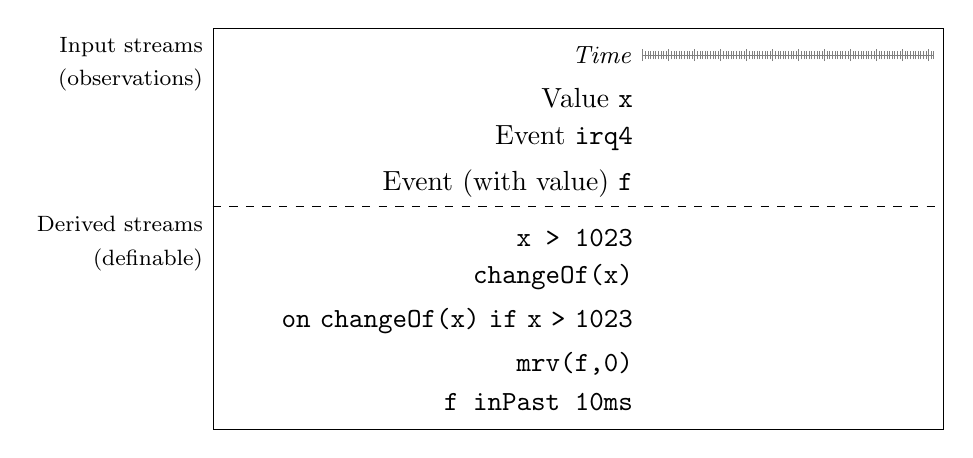
\begin{tikzpicture}

\matrix[column sep = 0.5em, draw] (m) {
  \node[anchor = east] {\small \textit{\textrm{Time}}}; \& \draw[help lines] (0,-0.05) grid[xstep=0.033] (3.7,0.05);
     \draw[gray] (0,-0.075) grid[xstep=0.33] (3.7,0.075); \\[0.5ex]
  \node[anchor = east] (m-1-2) {Value \texttt{x}}; \& \timing[name=m-2-2] at (0,-0.15) {2D{998}N(x1)2D{42}3D{2012}3D{1280}DD{10}DD{1404}};\\
%
  \node[anchor = east] (m-1-3) {Event \texttt{irq4}};
    \& \timing[name=m-2-3] at (0,-0.15) {ZZZ \n{} Z \n{} ZZZZ \n{} ZZ \n{} ZZZ \n{} Z}; \\
%
  \node[anchor = east] (end-inputs) {Event (with value) \texttt{f}};
    \& \timing[name = end-inputs-2] at (0,-0.15) {Z \n{17} ZZZZZZZ \n{98} Z \n{0} ZZZZ \n{23} Z}; \\[0.5em]
%
     \node[anchor = east] (m-1-5) {\texttt{x > 1023}};
  \& \timing[name=m-2-5] at (0,-0.15) {4L 6H 2L 2H}; \\
%
     \node[anchor = east] (m-1-6) {\texttt{changeOf(x)}};
  \& \timing[name=m-2-6] at (0,-0.15) {2Z \n{} 2Z \n{} 3Z \n{} 3Z \n{} 2Z \n{} 2Z}; \\
%
     \node[anchor = east, text width = 14.5em, align = right] (m-1-7) {
          \texttt{\textbf{on} changeOf(x) \textbf{if} x > 1023}};
  \& \timing[name=m-2-7] at (0,-0.15) {4Z \n{} 3Z \n{} 3Z 2Z \n{} 2Z}; \\
%
     \node[anchor = east] (m-1-8) {\texttt{mrv(f,0)}};
  \& \timing[name=m-2-8] at (0,-0.15) {D{0} 7D{17} D{98} 4D{0} D{23}}; \\
%
     \node[anchor = east] (m-1-9) {\texttt{f inPast 10ms}};
  \& \timing[name=m-2-9] at (0,-0.15) {L 2H 5L 3H 2L H}; \\
%
 };

\path[draw, dashed] (m.west|-end-inputs.south) edge (m.east|-end-inputs.south);

\path (m.north west) node[anchor = north east, align = right]
{\footnotesize{Input streams} \\ \footnotesize{(observations)}};

\path (m.west|-end-inputs.south) node[anchor = north east, align = right] {
  \footnotesize{Derived streams} \\ \footnotesize{(definable)}};

\end{tikzpicture}

  \caption{Visualization of \gls{tessla} stream model, taken from~\cite{Decker2016}}
\label{fig:chap2:sec_tessla:streams}
\end{figure}

The syntax of \gls{tessla} is concise, but can be used to define complex functions and specifications:

\begin{align*}
  spec\ \text{::= } &\textttbf{define } name[\textttbf{:}\ stype]\ \textttbf{:= } texpr |\\
                    & \textttbf{out } texpr |
                    spec\ spec\\
  texpr\ \text{:= } & expr[\textttbf{:}\ type] \\
  expr\ \text{:= }  & name \mid literal \mid name\textttbf{(}texpr(\textttbf{, }texpr)^*\textttbf{)}\\
  type\ \text{:= } & btype \mid stype \\
  stype\ \text{:= } & \textttbf{Signal<}btype\textttbf{>} \mid \textttbf{Events<}btype\textttbf{>}
\end{align*}

One of the main contributions of \gls{tessla} is the syntax which mimics modern programming languages and diverges from more clasical approaches in \gls{rv} that use more formal specification languages typically based on logics or automata.
This is an important step to enable practitioners without a strong theoretical background to adopt \gls{rv} techniques in their workflow.
While \gls{rv} has a lot of mechanisms to express specifications they often lack the ability to be intuitively understood.

There are many specification languages like \gls{ltl}~\citep{Pnueli77}, \gls{rltl}~\citep{Leucker2007}, \gls{ctl}~\citep{Clarke82} and many others that are geared heavily toward scientific work and theoretic reasoning.
When introducing new concepts, like realtime, this trend keeps up and formalism like \gls{tltl} from~\cite{Raskin1997}, \gls{stl} from~\cite{Maler2004} and \gls{mtl} from~\cite{Koymans1990} provide theoretical foundations to reason about realtime properties but formulas using these logics are even harder to understand than their non realtime counterparts.

One approach to make \gls{rv} more usage friendly is \gls{salt} presented in~\cite{Bauer2006} which acts as a frontend language to the more formal specification languages and can be translated into them.
\Gls{salt} unifies many different mechanisms, like specification patterns, nested scopes, exceptions, regular expressions and realtime.
\Cref{listing:salt_example} shows an example specification in \gls{salt} taken and adapted from~\cite{Dwyer1999} which specifies that on all three floors in a building, calling the elevator at floor \(\mathit{i}\) implies that it may pass at most two times at that floor without opening its doors, and that it must finally open its doors at that floor within 60 seconds.

\begin{lstlisting}[float,breaklines=true,label=listing:salt_example,caption={[Example \gls{salt} specification with realtime operators]An example specification in the \gls{salt} language taken from \cite{Bauer2006} defining behaviour of an elevator.}]
define max_twice_at_floor_before_open(i) := always (occurring[<=2] atfloor_$i$ between inclusive optional call_$i$ , exclusive optional open_$i$)
define max_60s_before_open(i) := always (call_$i$ implies eventually timed[<=60.0] open_$i$)
assert allof enumerate[1..3] as floor in max_twice_at_floor_before_open(floor) and max_60s_before_open(floor)
\end{lstlisting}

This specification shows, how \gls{salt} specifications are more intuitively understandable than logic formulas, for example by allowing to split the formula in multiple parts and assign meaningful identifiers to subformulas.

\Gls{tessla} and the runtime implemented in this thesis aim to combine many of the aspects that were presented in this Chapter: An understandable specification language like \gls{salt} that is able to express realtime properties, using streams of data as a central element like \gls{lola}, incorporate techniques from \gls{cep} like BeepBeep, and distribute the montitoring to many processors using Erlang and the actor model as shown in \cite{Attard2016}.

\section{Trace Data}
\label{sec:related:traces}

As in \gls{rv} we talk about monitoring of properties over traces, another important aspect is how traces can be extracted from a running program.
Many \gls{rv} tools solve this problem by using a technique called \emph{interweaving}: The code of the monitored program is changed in a way that the monitor becomes part of it, therefore the monitor becomes part of the program and has explicit access to the state of the running system.
Examples for this approach are AspectJ~\cite{Kiczales2001} and DiSL~\cite{Marek2012} for Java, and \gls{rmor}~\cite{Havelund2008} and \gls{rithm}~\cite{Navabpour2013} for C.
This approach is not feasible for the goals of the \gls{tessla} runtime, because we seek the portabilty that enables users to monitor multiple kinds of systems.

Therefore we are looking for ways to manipulate programs in a general way to emit trace data.

As a first step we seeked other projects to extract traces of data that can be used to evaluate the implemented runtime.
While there are many benchmarks available to test monitoring tools we were not able to find any that satisfied all of the characteristics that are needed for an evaluation of \gls{tessla}.
The next sections lists some of the benchmarks and evaluation tools that were surveyed and concludes with a tool that enabled the generation of suitable trace data.

\subsection{General Benchmarks for \glsentryname{rv} Tools}

The field of \gls{rv} lacks a common specification language and can be expanded to a wide variety of different properties to verify.
Therefore it is no surprise that there is no common benchmark that is applicable to all tools.
Nonetheless some benchmarks are occasionally used to compare the expressiveness of a new \gls{rv} tool.

The DaCapo benchmark~\citep{Blackburn2006} was introduced as a general purpose benchmark for the Java language.
It turned out that it can be used to benchmark monitor implementations and trace collection tools~\citep{Wu2016,Chen2007,Marek2012}.
Since Java was not the target architecture of our runtime the DeCapo benchmark was not used for the evaluation in this thesis.

The works in~\cite{Dwyer1999} can be seen as a benchmark for the expressiveness of a specification language.
It categorizes commonly monitored porperties into so called patterns like \emph{precedence}, \emph{absence} and \emph{response}.
While it would be valuable to test \gls{tessla} and the implemented runtimes against these patterns this would be a two step process.
First each pattern would have to be checked, if and how it could be expressed as a \gls{tessla} specification.
As a second step, if the pattern can be expressed, test trace data would have to be generated and only then the runtime could be evaluated using that pattern.
Since this thesis does not work on the \gls{tessla} language definition but only on the runtime we decided not to pursue this gial.

Another interesting project for evaluation of offline monitoring tools is TraceBench presented in~\cite{Zhou2014}.
TraceBench is a big set of traces collected from a distributed system running \gls{hdfs}.
During the collection errors of different categories were deliberately introduced, like network timeouts or data corruption.
The generated traces are organized in a hierarchy: if an event is produced as the effect of another event, for example a function call that leads to another function call, the second event is a child of the first.
Furthermore the traces contain the beginning and end of each event as a timestamp, making the traces suitable for \gls{tessla}.
Unfortunately it seems that the generated trace data has a problem: since events are produced in a distributed system the timestamps are faulty, for example some events started before their parent event.
Furthermore \gls{tessla} doesn't have a mechanism to express nested events as of now, meaning the traces would need to be manipulated before they could be used.

As a final benchmark we evaluated the \gls{crv}~\citep{Reger2016}.
\Gls{crv} has collected a set of benchmarks especially developed for the usage in monitoring algorithms.
It consists of three tracks: Java, C and offline.
While the C and offline track would have been very interesting the benchmarks don't contain any realtime properties.
Since the realtime fragment is an important part of \gls{tessla} we decided that the benchmark wasn't appropriate either.

\subsection{Tools to Generate Traces}

Since no suitable benchmark could be found the next step was to search for a tool that can be used to generate apropriate traces from programs during execution.
These tools can be categorized into static and dynamic instrumentation tools: static tools transform the source code of a program during compilation to include logging statements, dynamic ones only work at runtime and are not involved in the compilation process.

\subsection{CIL}

\Gls{cil} \cite{Necula2002} is a tool to write source-to-source transformations for C programs, therefore it is a static instrumentation tool.
\Gls{cil} implements ``a highly-structured clean subset of C'' in the OCaml language.
\Gls{cil} transforms a C program into an intermediate representation in OCaml.
\Gls{cil} will then apply transformations that are supplied by the programmer to the intermediate representation.
When all transformations are applied the program is written back as a normal C program.

Since \gls{cil} is able to represent the complete C90 standard and also extensions that are commonly used like the ones from GNU C, this tool can be used to write an instrumentation pass for the use case of trace generation.
The main reason that \gls{cil} was not used is that \gls{cil} only supports C and in this thesis we seek a tool that could be used on a variety of programming languages.

\subsection{Google XRay}

Google XRay~\cite{Berris2016} is a function call tracing system for C and \CC.
It is mainly a static instrumentation tool but has some aspects of a dynamic tool.
While XRay requires the orginal source code to be instrumented, the tracing functionality can be turned off at runtime which minimizes overhead.
XRay works by inserting a series of no-ops after function entry points and before return points.
At runtime a library that is part of XRay can then patch these no-ops with instructions to call a log function if tracing is enabled.
This rather complex mechanism is chosen to enable a minimal overhead which was a main requirement for the development of XRay.

XRay is at the moment implemented as a set of patches onto \gls{gcc} but is planned to be migrated to \gls{llvm}.
In typical usage scenarios XRay leads to an overhead of around 20\% to 40\%.

While XRay looks like a promising all-in-one solution to trace collection it only supports the instrumentation of function entrys and exits.
For our instrumentation we wanted to explore the possibility to also trace other events and maybe even allow to attach conditions when an event is actually logged.
As an example consider logging an event whenever a variable is assigned more than once in a single function call.

\subsection{DTrace}

\Cite{Cantrill2004} presents DTrace, a ``facility for dynamic instrumentation of production systems''.
DTrace relies on support from the Kernel of the operating system and does require specific compilation settings for some instrumentations.
DTrace includes a language to specify instrumentations called D.

To use DTrace one has to specify \emph{probes} in the D language.
A \emph{probe} consists of probe descriptions, a predicate and action statements.
The probe descriptions specifies the kind of instrumentation it provides and the modules and functions the probe should be applied to.
The predicate can be used to skip the invocation of the probe if certain conditions are not met.
Action statements contain code that is executed hwen the probe is called.

\Cref{listing:dtrace_spec} shows a DTrace specification with two probes.
The first probe is invoked everytime the instrumetned program calls the \lstinline{read} function provided by the operating system and assigns the current timestamp to a variable.
The second probe is invoked everytime the \lstinline{read} function returns and logs the time used by the \lstinline{read} function before returning.
The predicate of the second probe checks if the variable \lstinline{t} has been assigned.

\begin{lstlisting}[showstringspaces=false,language=C,float,label=listing:dtrace_spec, caption={A DTrace specification in the D language specifying two probes}]
syscall::read:entry {
  self->t = timestamp;
}

syscall::read:return
/self->t/ {
  printf("%d/%d spent %d nsecs in read\n",
    pid, tid, timestamp - self->t);
}
\end{lstlisting}

DTrace offers a variety of instrumentation types, called \emph{providers} in DTrace, \lstinline{syscall} from the previous example being one of them.
Interesting for our research is the \emph{pid} provider which enables the instrumentation of arbitrary instructions in a specified process.
The \emph{pid} provider can be used to log function entrys and exits of every function in a program.

\Cite{Rosenberg2016} builds upon DTrace to build a \gls{rv} framework.
It produces automaton based monitors in the D language from specifications written in \gls{ltl}.
To do so it connects atomic propositions of the formula with observable events that are represented as probes in DTrace.
Whenever a probe is invoked it updates the state of the automaton as specified with the action statements of that probe.

\subsection{LLVM}
\label{sec:related:traces:llvm}

\Gls{llvm}~\cite{Lattner2004} is a compiler framework that allows program analysis and transformation.
The compilation process of \gls{llvm} is seperated into three parts: a front-end, a middle-end and a back-end.
A front-end is responsible for translating a source language, for example C or \CC, into \gls{llvm} \gls{ir}, a strongly typed \gls{risc} instruction set which is independent from the target platform.
The middle-end performs source-to-source transformations on the \gls{ir} that can perform analysis or optimizations.
Such transformations are called \emph{compiler passes} and are independent of the source language.
The back-end is then used to transform the \gls{ir} into native machine code for the target platform.

The \emph{compiler pass} on top of \gls{ir} provides a good abstraction as a base for an instrumentation to generate traces.
Since a pass works on \gls{ir} and not on the source language itself the instrumentation can be used for every language that has an \gls{llvm} front-end.
At the time of writing there is a large collection of such frontends for many languages, including C, \CC, Objective-C, Swift, Haskell, Ruby and many more\footnote{\url{http://llvm.org/ProjectsWithLLVM/}}.

Furthermore a compiler pass can work on all parts of a program: whole modules (think classes in C), function definitions, variable reads and writes, memory allocation and others.
The building block of \gls{ir} programs in \gls{llvm} are the so called \emph{instructions}\footnote{\url{http://llvm.org/docs/doxygen/html/classllvm_1_1Instruction.html}}.
Each statement from a source language is represented as such an instruction.
A \emph{compiler pass} is able to examine instructions, change or reorder them and generate new instructions and insert them appropriately.

Due to the great flexibility that a \emph{compiler pass} offers we chose this approach for the instrumentation pass.
The implementation details can be seen in \Cref{sec:implementation:instrumentation}.


% !TEX root = ../thesis.tex
\chapter{Preliminaries}
\label{sec:definitions}

In this chapter we will define concepts that are used in \Cref{sec:behaviours} to reason about the implemented runtime.

While the \gls{tessla} specification itself defines a set of semantics, for this thesis we will slightly alter some of it and add some new definitions based on them.
This is necessary to reason about the specifics how the runtime is built (Note that \gls{tessla} doesn't define an operational semantic, therefore we will define our own) and how it behaves.

\section{Time}
\label{sec:definitions:time}

\gls{tessla} has a model of continuous time, where timestamps \(\pi \in \mathbb{T} \) are used to represent a certain point in time and \(\mathbb{T}\) has to be isomorphic to \(\mathbb{R}\).

\section{Transducers}
\label{sec:definitions:transducers}

Fundamentally \gls{tessla} is a special kind of a transducer.
Therefore in this section we will define a model of transducers which can be used to reason about the evaluation of a \gls{tessla} specification.

A transducer is a system, which consumes an input and produces an output.
Let \(\Phi, \Gamma\) be two alphabets and \(\epsilon\) the empty word.

\begin{definition}[name = Transducer]\label{def:transducer}
  A transducer \(t\) is a relation \(t \subseteq \Phi^* \times \Gamma^*\), \(\Phi\) is called the input alphabet, \(\Gamma\) the output alphabet.
\end{definition}

\gls{tessla} specifications are deterministic for any input, meaning they should produce the same output for the same input.

\begin{definition}[name = Deterministic Transducer]\label{def:deterministic_transducer}
  A deterministic transducer relates each input to at most one output.
\end{definition}

\begin{exmp}[name = Deterministic and Nondeterministic Transducers]
  \(t_d = \{(a,1),(b,2),(ab,12),(ba,21)\}\) is a deterministic transducer, \(t_{nd} = \{(a,1),(a,2)\}\) is nondeterministic, because it relates input \(a\) to both outputs \(1\) and \(2\).
\end{exmp}

Transducers can furthermore be categorized as synchronous, asynchronous, causal and clairvoyant transducers:
synchronosity is a property over the behaviour of a transducer when it's consuming input per element.
If it is synchronous, it will produce an output element for each input element.

\begin{definition}[name = Synchronous Transducer]\label{def:synchronous_transducer}
Let \(\vec{\imath} \in \Phi^*, i \in \Phi, \vec{o} \in \Gamma^*, o \in \Gamma\).
  A transducer \(t\) is called synchronous, when it satisfies, that:
  if \( (\vec{\imath}\circ i,\vec{o}\circ o) \in t\)
  then \( (\vec{\imath}, \vec{o}) \in t \)
\end{definition}

An asynchronous transducer can produce zero, one or many outputs for each input it consumes.

\begin{definition}[name = Asynchronous Transducer]\label{def:asynchronous_transducer}
  Let \(\vec{\imath}\in \Phi^*, i \in \Phi,\vec{o} \in \Gamma^*\).
  A transducer \(t\) is called asynchronous when it satisfies the formula:
  if \((\vec{\imath}\circ i, \vec{o}) \in t \)
  then \(\exists \vec{o'},\vec{o''} \in \Gamma^*\text{ so that } \vec{o} = \vec{o'}\circ\vec{o''} \text{ and } (\vec{\imath},\vec{o'}) \in t \)
\end{definition}

\begin{exmp}[name = Synchronous and Asynchronous Transducers]
  \(t_s = \{(a,1),(b,2),(ab,12),(ba,21)\}\) is a synchronous transducer, \(t_{as} = \{(a,\epsilon),(ab,12)\}\) is asynchronous.
\end{exmp}

A causal transducer is one, where the output depends only on consumed inputs and not on future inputs:

\begin{definition}[name = Causal and Clairvoyant Transducers]\label{def:causal_transducer}
  A transducer \(t\) is called causal, when it satiesfies, that:
  if \((\vec{\imath},\vec{o}) \in t \)
  then \( \forall \vec{\imath'} \in \Phi^* \text{ with } (\vec{\imath} \circ \vec{\imath'}, \vec{o'}) \in t \)
  it holds, that \( \vec{o} \sqsubseteq \vec{o'} \)

  A transducer that isn't casual is called \emph{clairvoyant}.
\end{definition}


\begin{exmp}[name = Causal and Clairvoyant Transducers]
  \(t_{cl} = \{(a,1),(b,2),(ab,12),(ba,21)\}\) is a causal transducer, because each output only depends on the inputs seen upto that point, \(t_{cl} = \{(a,1),(ab,22),(aa,11)\}\) is clairvoyant, because the output when the letter \(a\) is seen depends on the next input.
\end{exmp}

When talking about transducers, it is interesting to know if two transducers are \emph{equivalent}.
There are multiple possible definitions for equivalence of transducers, we will look at two, which are interesting for this thesis.
In the following \(\sigma_i\) is used to get the element at position \(i\) and \(\sigma_{[i,j]}\) to get the infix of \(\sigma\) which starts at position \(i\) and ends at position \(j\) (With \(0\) as the index of the first element).

\begin{definition}[name = Asynchronous equivalence of Transducers]\label{def:async_equivalence_transducer}
  Let \(t_1, t_2\) be two asynchronous transducers from \(\Phi^*\) to \(\Gamma^*\).
  They are called \emph{asynchronous equivalent}, written \(t_1 \equiv_a t_2\), if they satisfy: \\
  \(\forall \sigma \in \Phi^*\):
  \begin{itemize}
    \item \(\forall (\sigma_{[0,k]}, \vec{o}) \in t_1\): \(\exists k' \geq k \text{ with } (\sigma_{[0,k']}, \vec{o'}) \in t_2\) and \(\vec{o} \sqsubseteq \vec{o'}\)
    \item and \(\forall (\sigma_{[0,k]}, \vec{o}) \in t_2\): \(\exists k' \geq k \text{ with } (\sigma_{[0,k']}, \vec{o'}) \in t_1\) and \(\vec{o} \sqsubseteq \vec{o'}\)
  \end{itemize}
\end{definition}

\begin{lemma}[name=Asynchronous equivalence is an equivalence Relation]\label{lemma:async_equivalence_is_equivalence_relationship}
  Asynchronous equivalence is symmetric, reflexive and transitive.
\end{lemma}
\begin{proof}$ $\newline
    Symmetry is trivial, since the second part of the definition is requiring it.\\
    Reflexivity is also trivial, for \((\sigma_{[0,k]}, \vec{o})\) select \(k' = k\).\\
    For transitivity:
    \begin{itemize}[label = {}]
      \item Let \(t_1 \equiv_a t_2\), \(t_2 \equiv_a t_3\).
      \item First case:
        \begin{align*}
          &\text{Since } t_1 \equiv_a t_2:\ \forall (\sigma_{[0,k_1]}, \vec{o_1}) \in t_1: \\
          &\hspace{2em} \exists k_2\ \text{such, that } (\sigma_{[0,k_2]}, \vec{o_2}) \in t_2\ \text{with } \vec{o_1} \sqsubseteq \vec{o_2} \\
          &\hspace{2em} \text{and since } t_2 \equiv_a t_3 \\
          &\hspace{4em} \exists k_3\ \text{such, that } (\sigma_{[0,k_3]}, \vec{o_3}) \in t_3\ \text{with } \vec{o_2} \sqsubseteq \vec{o_3}\\
          &\hspace{4em} \text{With } \vec{o_1} \sqsubseteq \vec{o_2} \sqsubseteq \vec{o_3}\ \text{it follows, that } t_1 \equiv_a t_3
        \end{align*}
      \item The second case works the same, just change \(t_1\) and \(t_3\).
    \end{itemize}
\end{proof}

\begin{exmp}[name = Asynchronous equivalence of Transducers]
  Let \(\Phi = \{a\}, \Gamma = \{1\}\) and \\
  \begin{align*}
    &t_1 = \{&&(a,\epsilon),  &&(aa,\epsilon),  &&(aaa,111)   &\} \\
    &t_2 = \{&&(a,1),         &&(aa,1),         &&(aaa,111)   &\} \\
    &t_3 = \{&&(a,\epsilon),  &&(aa,1),         &&(aaa,11)    &\}\\
  \end{align*}
  All three transducers are asynchronous and causal.
  Let's see which ones are asynchronous equivalent:

  \(t_1 \stackrel{?}{\equiv}_a t_2\)
  \begin{align*}
    &(a,\epsilon)  &&\in t_1, k = 1 &\rightarrow k' = 1, &(a,1)     \in t_2, &\epsilon  &\sqsubseteq 1 \\
    &(aa,\epsilon) &&\in t_1, k = 2 &\rightarrow k' = 2, &(aa,1)    \in t_2, &\epsilon  &\sqsubseteq 1 \\
    &(aaa,111)     &&\in t_1, k = 3 &\rightarrow k' = 3, &(aaa,111) \in t_2, &111       &\sqsubseteq 111 \\
    &(a,1)         &&\in t_2, k = 1 &\rightarrow k' = 3, &(aaa,111) \in t_1, &1         &\sqsubseteq 111 \\
    &(aa,1)        &&\in t_2, k = 2 &\rightarrow k' = 3, &(aaa,111) \in t_1, &1         &\sqsubseteq 111 \\
    &(aaa,111)     &&\in t_2, k = 3 &\rightarrow k' = 3, &(aaa,111) \in t_1, &111       &\sqsubseteq 111 \\
  \end{align*}
  \(\Rightarrow t_1 \equiv_a t_2\)

  \(t_1 \stackrel{?}{\equiv}_a t_3\)
  \begin{align*}
    &(aaa,111)     \in t_1, k = 3 \rightarrow \not\exists k'
  \end{align*}
  \(\Rightarrow t_1 \not\equiv_a t_3\)

  Because of \Cref{lemma:async_equivalence_is_equivalence_relationship} \(\Rightarrow t_2 \not\equiv_a t_3\).

\end{exmp}

\section{Timed Transducers}
\label{sec:definitions:timed_transducer}

For the second kind of equivalence we need to introduce \emph{timed sequences}, originally introduced as timed words in~\cite{Alur1994}, and \emph{timed transducers}.
Note that timed sequences don't have to be monotonically increasing like in the original definition.
Quite on the contrary the unorderdness of outputs is an important key principle to much of the later work as you will see.

Let \(\mathbb{T}\) be a timing model that is isomorphic to \(\mathbb{R}\).
For the examples we will use \(\mathbb{R}\) for \(\mathbb{T}\).

\begin{definition}[name = Timed Sequence]\label{def:timed_sequence}
  A sequence is called timed, if every element of it is associated with a timestamp: \(\sigma \in {(\Gamma\times\mathbb{T})}^*\).
  For bravety a timed sequence can be written with the timestamps as the index of the elements: \(\sigma = e_0e_{0.5}e_1 \).\\
  The function
  \[\mathit{timed: } {(\Gamma \times \mathbb{T})}^* \rightarrow {(\Gamma \times \mathbb{T})}^* \]
  reorders a timed sequence \(\sigma\) by its timestamps, such that:
  \[ \forall i,j \in \mathbb{N}:\text{ if } i < j \text{ then } \pi_i < \pi_j \text{ with } (o_i, \pi_i) = \sigma_i \text{ and } (o_j, \pi_j) = \sigma_j \]
  The function
  \[\mathit{upto: } \mathbb{T} \times {(\Gamma\times\mathbb{T})}^* \rightarrow {(\Gamma\times\mathbb{T})}^*\]
  removes all elements from a timed sequence, that have a timestamp bigger than the first argument.\\
  The function
  \[\mathit{maxTime: } {(\Gamma\times\mathbb{T})}^* \rightarrow \mathbb{T} \]
  returns the biggest Timestamp in a timed sequence.
\end{definition}

\begin{exmp}[name=Functions on Timed Sequences]
Let \(\sigma = a_1a_{0.5}a_{1.5}a_0\).\\
  Then is
    \begin{align*}
      &\mathit{timed} (\sigma) = a_0a_{0.5}a_1a_{1.5}\ \\
      &\mathit{upto} (1.3,\sigma) = a_1a_{0.5}a_0 \\
      &\mathit{maxTime} (\sigma) = 1.5
    \end{align*}
\end{exmp}

\begin{definition}[name = Monotonicity of Timed Sequences]\label{def:monotonicity_timed_sequences}
  A timed sequence \(\sigma\) with alphabet \(\Phi\) is called monotonic,
  if \( \mathit{timed}(\sigma) = \sigma\)
\end{definition}

\begin{definition}[name = Timed Transducer]\label{def:timed_transducer}
  A timed transducer \(t\) with input alphabet \(\Phi\) and output alphabet \(\Gamma\) works on monotonic, timed sequences as inputs and has timed sequences as outputs:
  \[t \subset {\left(\Phi \times \mathbb{T}\right)}^* \times {\left(\Gamma \times \mathbb{T}\right)}^*\]
\end{definition}

\begin{exmp}[name=Timed Transducers]
  \begin{align*}
    &\text{Let } \Phi = \{a\}, \Gamma = \{b\}.\\
    &t_{tsc} = \{(a_0, b_0),(a_0a_1, b_0b_1)\}\ \text{is a timed, causal and synchronous transducer.}\\
    &t_{tac} = \{(a_0, \epsilon),(a_0a_1, b_0b_1)\}\ \text{is a timed, causal and asynchronous transducer.}
  \end{align*}
\end{exmp}

For later theoretic work we have to restrict timed transducers.

\begin{definition}[name = Boundedness of Timed Transducers]\label{def:boundedness_timed_transducer}
  A timed transducer \(t\) with input alphabet \(\Phi\) and output alphabet \(\Gamma\) is called bounded, if it satisfies:
  \begin{align*}
    &\forall \sigma \in {(\Phi \times \mathbb{T})}^*:\\
    &\hspace{2em}\text{if } (\sigma_{[0,k]}, \vec{o}) \in t\\
    &\hspace{2em}\text{then }\exists k' > k\ \text{with}\\
    &\hspace{4em}(\sigma_{[0,k']}, \vec{o} \circ \vec{o'}) \in t\\
    &\hspace{4em}\text{and} \forall k'' > k'\ \text{with } (\sigma_{[0,k'']}, \vec{o}\circ\vec{o'}\circ\vec{o''}) \in t\ \text{it holds, that}\\
    &\hspace{6em}\mathit{upto}(\mathit{maxTime}(\vec{o}), \mathit{timed}(\vec{o}\circ\vec{o'})) = \mathit{upto}(\mathit{maxTime}(\vec{o}), \mathit{timed}(\vec{o}\circ\vec{o'}\circ\vec{o''}))
  \end{align*}
\end{definition}
Based on the definitions we can define an equivalence relationship on bounded timed transducers.

\begin{definition}[name = Observational Equivalence]\label{def:observational_equivalence}
  Let \(t_1, t_2\) be two bounded timed transducers with input alphabet \(\Phi\) and output alphabet \(\Gamma\).
  They are called \emph{observational equivalent}, written \(t_1 \equiv_o t_2\), if they satisfy:
  \begin{align*}
    &\forall \sigma \in {(\Phi\times\mathbb{T})}^*:\\
    &\hspace{2em}\forall (\sigma_{[0,k]}, \vec{o}) \in t_1: \exists k', k'' \geq k\ \text{such that}\\
    &\hspace{4em}(\sigma_{[0,k']}, \vec{o} \circ \vec{o'}) \in t_1\\
    &\hspace{4em}\text{and } (\sigma_{[0,k'']}, \vec{o_2}) \in t_2\\
    &\hspace{4em}\text{and } \mathit{timed}(\mathit{upto}(\mathit{maxTime}(\vec{o}),\vec{o} \circ \vec{o'} )) = \mathit{timed}(\mathit{upto}(\mathit{maxTime}(\vec{o}),\vec{o_2}))
  \end{align*}
  and the same for switched \(t_1, t_2\).
\end{definition}

What does observational equivalence between two transducers intuitively mean?
It means that two transducers eventually produce the same output values for the same timed inputs, maybe in a different order, but with the same timestamps, which is very important.
Since the values are associated with timestamps the outputs can be reordered by them and therefore be exactly equal.

\begin{lemma}[name=Observational Equivalence is an Equivalence Relationship for Bounded Transducers]\label{lemma:observational_equivalence_equivalence_relationship}
  \(\equiv_o\) is symmetric, reflexive and transitive for bounded timed transducers.
\end{lemma}
\begin{proof}$ $\newline
  Let \(t_1, t_2, t_3\) be bounded timed transducers.
  Symmetry follows directly from the definition.\\
  Reflexivity: For \((\sigma_{[0,k]}, \vec{o})\) select \(k' = k''\) as the k, for which the transducer is bounded for that input.\\
  Transitivity:
  \begin{itemize}
    \item Let \(t_1 \equiv_o t_2\), \(t_2 \equiv_o t_3\).
    \item First case:
      \begin{align*}
        &\text{Since } t_1 \equiv_o t_2:\ \forall (\sigma_{[0,k_1]}, \vec{o_1}) \in t_1: \\
        &\hspace{2em} \exists k_1', k_2 > k_1\ \text{with } (\sigma_{[0,k_1']}, \vec{o_1}\circ\vec{o_1'}) \in t_1\ \text{and } (\sigma_{[0,k_2]}, \vec{o_2}) \in t_2 \\
        &\hspace{4em} \text{with } \mathit{timed}(\mathit{upto}(\mathit{maxTime}(\vec{o_1}),\vec{o_1} \circ \vec{o_1'} )) \\
        &\hspace{8em} = \mathit{timed}(\mathit{upto}(\mathit{maxTime}(\vec{o_1}),\vec{o_2})) & (\star)\\
        &\hspace{2em} \text{and since } t_2 \equiv_o t_3: \exists k_2', k_3 > k_2\ \text{with } (\sigma_{[0,k_2']}, \vec{o_2}\circ\vec{o_2'}) \in t_2 \\
        &\hspace{4em} \text{and } (\sigma_{[0,k_3]}, \vec{o_3}) \in t_3 \\
        &\hspace{6em} \text{with } \mathit{timed}(\mathit{upto}(\mathit{maxTime}(\vec{o_2}),\vec{o_2} \circ \vec{o_2'} )) \\
        &\hspace{10em} = \mathit{timed}(\mathit{upto}(\mathit{maxTime}(\vec{o_2}),\vec{o_3})) & (\star\star)\\
        &\hspace{2em} \mathit{maxTime}(\vec{o_1})\ \text{has to be smaller then}\mathit{maxTime}(\vec{o_2}) \\
        &\hspace{4em} \text{else } (\star)\ \text{couldn't hold, therefore, combined with boundedness and }(\star\star): \\
        &\hspace{4em} \mathit{timed}(\mathit{upto}(\mathit{maxTime}(\vec{o_1}),\vec{o_2} )) \\
        &\hspace{8em} = \mathit{timed}(\mathit{upto}(\mathit{maxTime}(\vec{o_1}),\vec{o_3})) \\
        &\text{which concludes }\mathit{timed}(\mathit{upto}(\mathit{maxTime}(\vec{o_1}),\vec{o_1} \circ \vec{o_1'} ))\\
        &\hspace{4em} = \mathit{timed}(\mathit{upto}(\mathit{maxTime}(\vec{o_1}),\vec{o_3}))
      \end{align*}
    \item The second case works the same, just switch \(t_1\) and \(t_3\).
  \end{itemize}
\end{proof}


\begin{exmp}[name=Observational Equivalence]\label{exmp:observational_equivalence}
  Let
  \begin{align*}
    &t_1 = \{&&(a_0, \epsilon),   &&(a_0a_1, b_1),      &&(a_0a_1a_2, b_1b_2b_0)  &\} \\
    &t_2 = \{&&(a_0, \epsilon),   &&(a_0a_1, \epsilon), &&(a_0a_1a_2, b_2b_1b_0)  &\} \\
    &t_3 = \{&&(a_0, b_0),        &&(a_0a_1, b_0),      &&(a_0a_1a_2, b_2b_1)     &\}
  \end{align*}
  All three are causal, asynchronous timed transducers.

  Let's see which ones are observational equivalent:

  \(t_1 \stackrel{?}{\equiv}_o t_2\)
  \begin{itemize}[label={}]
    \item \((a_0, \epsilon)             \in t_1, k = 1, \mathit{maxTime}(\epsilon) = 0\)
      \begin{itemize}[label={}]
        \item \(\rightarrow k' = 1, (a_0, \epsilon)     \in t_1\)
        \item \(\rightarrow k'' = 1, (a_0, \epsilon)     \in t_2\)
      \end{itemize}
    \item \((a_0a_1, b_1)               \in t_1, k = 2, \mathit{maxTime}(b_1) = 1\)
      \begin{itemize}[label={}]
        \item \(\rightarrow k' = 3, (a_0a_1a_2, b_1b_2b_0)    \in t_1\)
        \item \(\rightarrow k'' = 3, (a_0a_1a_2, b_2b_1b_0)    \in t_2\)
        \item \(\mathit{timed}(\mathit{upto}(1, b_1b_2b_0)) = b_0b_1 = \mathit{timed}(\mathit{upto}(1, b_2b_1b_0))\)
      \end{itemize}
    \item \((a_0a_1a_2, b_1b_2b_0)               \in t_1, k = 3, \mathit{maxTime}(b_1b_2b_0) = 2\)
      \begin{itemize}[label={}]
        \item \(\rightarrow k' = 3, (a_0a_1a_2, b_1b_2b_0)    \in t_1\)
        \item \(\rightarrow k'' = 3, (a_0a_1a_2, b_2b_1b_0)    \in t_2\)
        \item \(\mathit{timed}(\mathit{upto}(2, b_1b_2b_0)) = b_0b_1b_2 = \mathit{timed}(\mathit{upto}(2, b_2b_1b_0))\)
      \end{itemize}
    \item \((a_0, \epsilon)               \in t_2, k = 1, \mathit{maxTime}(\epsilon) = 0\)
      \begin{itemize}[label={}]
        \item \(\rightarrow k' = 1, (a_0, \epsilon)     \in t_2\)
        \item \(\rightarrow k'' = 1, (a_0, \epsilon)     \in t_1\)
      \end{itemize}
    \item \((a_0a_1, \epsilon)            \in t_2, k = 2, \mathit{maxTime}(epsilon) = 0\)
      \begin{itemize}[label={}]
        \item \(\rightarrow k' = 2, (a_0a_1, \epsilon)    \in t_2\)
        \item \(\rightarrow k'' = 2, (a_0a_1, b_1)    \in t_1\)
        \item \(\mathit{timed}(\mathit{upto}(0, \epsilon)) = \epsilon = \mathit{timed}(\mathit{upto}(0, b_1))\)
      \end{itemize}
    \item \((a_0a_1a_2, b_2b_1b_0)        \in t_2, k = 3, \mathit{maxTime}(b_2b_1b_0) = 2\)
      \begin{itemize}[label={}]
        \item \(\rightarrow k' = 3, (a_0a_1a_2, b_2b_1b_0)    \in t_2\)
        \item \(\rightarrow k'' = 3, (a_0a_1a_2, b_1b_2b_0)    \in t_1\)
        \item \(\mathit{timed}(\mathit{upto}(2, b_2b_1b_0)) = b_0b_1b_2 = \mathit{timed}(\mathit{upto}(2, b_1b_2b_0))\)
      \end{itemize}
  \end{itemize}
  \(\Rightarrow t_1 \equiv_a t_2\)

  \(t_1 \stackrel{?}{\equiv}_a t_3\)
  \begin{itemize}[label={}]
    \item \((a_0a_1a_2,b_1b_2b_0)      \in t_1, k=3, \mathit{maxTime}(b_1b_2b_0) = 2\)
      \begin{itemize}[label={}]
        \item \(\rightarrow k' = 3, (a_0a_1a_2, b_1b_2b_0)    \in t_1\)
        \item \(\rightarrow \not\exists (\vec{\imath}, \vec{o}) \in t_3\ \text{with } \exists n \in \mathbb{N}: \vec{o}_n = b_0\)
        \item \(\rightarrow \not\exists (\vec{\imath}, \vec{o}) \in t_3\ \text{with } \mathit{timed}(\mathit{upto}(2, b_1b_2b_0)) = b_0b_1b_2 = \mathit{timed}(\mathit{upto}(2,\vec{o}))\)
      \end{itemize}
  \end{itemize}
  \(\Rightarrow t_1 \not\equiv_a t_3\)\\
  If \(t_3\) weren't bounded (and therefore not finite) there would be no way to know, if it was equivalent to \(t_1\), because it could always produce a missing event at a later time.

  Because of \Cref{lemma:observational_equivalence_equivalence_relationship} \(\Rightarrow t_2 \not\equiv_a t_3\).

\end{exmp}

% \section{Labeled Timed Transducers}
% Maybe necessary, maybe not

\section{Events}
\label{sec:definitions:events}

Events are the atomic unit of information that all computations are based on.
There are three types of events: external, output and internal events.

The set of all events is denoted as \(E\).
Each event carries a value, which can be \emph{nothing} or a value of a type (types are formally defined in the \gls{tessla} specification, but aren't important for this thesis), a timestamp and the stream it's perceived on (for example a function call of a specific function or the name of an output stream).

The value of an event can be queried with the function \(\upsilon\), its timestamp with \(\mathit{time}\) and its stream with \(\mathit{stream}\).

\(E_e \subset E\) is the set of all external events, their stream corresponds to a specific trace.
\(E_o \subset E\) is the set of all output events, their stream is specified by an output name of the \gls{tessla} specification.
\(E_n \subset E\) is the set of all internal events.
Internal events are mostly an implementation detail, which denote steps of computation inside the runtime.
The stream of internal events is implicitly given by the node that produces the stream of the event.
Note that \(E_e, E_o, E_n\) are pairwise disjoint and \(E_e \cup E_o \cup E_n = E\).

\section{Streams}
\label{sec:definitions:streams}

Streams are a collection of events with specific characteristics.
While events are the atomic unit of information, streams represent the sequence of related events over time.

There are two kind of streams: signals, which carry values at all times, and event\-streams, which only hold values at specific times.
Eventstreams can be described by a sequence of events.
Signals can be described by a sequence of changes, where a change denotes that the value of a signal changed at a specific timestamp.
The only difference between a signal and an eventstreams is that signals always have a value while an eventstream may return \(\bot\) when queried for its value at a specific time, which denotes that no event happened at that time.
Based on the similarity of signals and eventstreams in the following we will mainly reason about eventstreams, but most things can also be applied to signals.

Formally a stream \(\sigma\) can be represented as the product of a sequence of events \(\langle e_1, \dots e_n\rangle\) where \(\mathit{time}(e_i) < \mathit{time}(e_{i+1}),\ \forall i < n \in \mathbb{N}\).
The set of all streams \(\Sigma\) is defined as all possible finite sequences of events \(\Sigma = \{\sigma | \sigma \in E^* \}\).
An external stream \(\sigma_e\) is a stream consisting only of external events, the set of all external streams is \(\Sigma_e = \{\sigma_e | \sigma_e \in E_e^*\} \times \mathbb{T}\).
Output and internal streams are defined analogous.

To get the event of a stream \(\sigma\) at a timestamp \(\pi\) it can be queried like a function: \(\sigma(\pi) = e\) with \(\mathit{time}(e) = \pi \).
When working with signals, the function will return the latest event that happened at or before t while an eventstream may return \(\bot\).
The progress of a stream, which is the timestamp of the last event that happened on them, can be obtained with \(\mathit{progress}(\sigma) = \pi \in \mathbb{T}\).
Internal and output streams can be queried for the node that produced them with \(\mathit{node}(\sigma) = n \in N\).

\section{Functions}
\label{sec:definitions:functions}

A \gls{tessla} specification consists of functions over streams.
Functions generate new streams by applying an operation on existing streams.
\gls{tessla} itself defines a syntax to write a specification, a set of types and a standard library of functions, but an implementation is free to choose the functions it supports.

An example function is \(\mathit{add}(S_D,S_D) \rightarrow S_D\): It takes two signals, which have to hold values of some numerical type, and produces a signal which holds values of the same type.
The produced stream can either be assigned to a named identifier (think: a variable) or consumed by another function (function composition).

Functions can be divided into three categories: pure, unpure and timing.
Pure functions, also called stateless, are evaluated only on the values their inputs have at the timestamp they are evaluated, therefore they don't have to remember a state and will only return events.
Unpure, or stateful, functions are evaluated over the values if its inputs at that timestamp and a state and will return not only new events but also an updated state.
As an example a function \emph{eventCount} has to \emph{remember} how many events already happened on it's input stream and increment that counter on every new event.
Timing functions are evaluated not only on the value of events but also on their timestamp and can also manipulate it:
While non timing functions will consume events at a specific timestamp and emit events with that timestamp, timing functions can emit events with a changed timestamp.
In this thesis we will only look at past time functions, meaning functions can only delay timestamps, therefore can't depend on future values.

Timing functions complicate the reasoning about schedules and causality and therefore aren't included in \Cref{sec:behaviours:without_timing}.
In \Cref{sec:behaviours:timing_functions} the conclusions of earlier sections will be extended to include timing functions.

\section{Nodes}
\label{sec:definitions:nodes}

Nodes are the atomic unit of computation for the evaluation of a \gls{tessla} specification.
A node implements a single function: there is an \emph{AddNode} which takes two input signals and produces a new signal.
Therefore a node is the concrete implementation of a function in a runtime for \gls{tessla} specifications.
The set of all nodes is called \(N\).
The function of a node \(n \in N\) is written as \(f_n\).

Each node has a set of inputs, which are either external or internal streams, and one output, which is either an internal or an output stream.
Nodes which have at least one external stream as an input are called \emph{sources}.
Nodes have a state, described in \Cref{sec:definitions:state}, which contains \gls{fifo} queues, provided by the Erlang platform, which buffer events from its inputs for later computation.

Every new event added to a queue has to have a bigger timestamp than the previous event added to the queue.
This means a queue has a kind of progress timestamp, which denotes the timestamp of the latest event added to it and which is strictly increasing over time.
Queues support the standard operators for lists like \(\mathit{hd}, \mathit{tl}, ++\) to respectively get the head, the tail or to append to the end.


\section{\glsentryname{tessla} Evaluation Engine}
\label{sec:definitions:eval_engine}

Because functions in \gls{tessla} specifications depend on other functions, and these dependencies have to be cycle free, the specification can be represented as a \gls{dag}, where the functions are vertices and the relationship between functions are edges.
This is exactly how the \gls{tessla} compiler outputs a specification.
One can now use the \gls{dag} of a \gls{tessla} specification to synthesize a system to evaluate it over inputs:
The vertices of the \gls{dag} become nodes representing the functions and the edges are the input and output streams between the nodes.
We will call this synthesized system an \emph{evaluation engine}.

When fed with inputs (or \emph{traces}) the engine will produce outputs.
The relationship between inputs and outputs that is produced can be seen as a timed transducer.
The input to an evaluation engine has to have strictly increasing timestamps.
This is needed to have a known progress which can be distributed through the system.
If inputs weren't ordered by their timestamp for example the absense of input events on a specific stream couldn't be detected because events could be present at a later position of the input trace.
Especially for offline monitoring this obviously is no problem because the traces can simply be reordered into a strictly increasing sequence, except when multiple input events are at the same timestamp.
This can be solved in two ways: either increase the timing precision when generating the traces or manipulate the timestamps in the traces by adding a minimal offset to them if they are equal to another timestamp.

To evaluate a specification over traces, the evaluation engine has process the events that were traced.
To do so the nodes have to run their computations until no more events are present (or the specification found an error in the trace).
This leads to the question in which order nodes should be scheduled to perform their computation.
We will use the term \emph{step} to denote that one node was scheduled and performed its computation.
While some schedules are simply not rational (think of unfairness and causality), there are many different schedules that are feasible.
It has to be proven that a chosen schedule produces the correct conclusions for a specification, else the evaluation engine is not valid.

An evaluation engine is run inside an environment.
The environment has knowledge over the state of the nodes, most important which nodes are enabled.
Based on that information the environment is responsible of feeding the trace data to the engine: only when no sources are enabled the next trace is added to the queue of an input node.
This ensures that the consumption of input signals is strictly ordered by timestamp, which is important as we will see in \Cref{sec:behaviours}.


\section{\glsentryname{tessla} Functions}
\label{sec:definitions:tessla_functions}

\gls{tessla} puts no restrictions on the semantics of functions other than that they have to work on streams or constants and produce streams, but allows to restrict them for evaluation approaches.
We are taking advantage of that to categorize functions based on how or if at all they can be encoded in our evaluation approach.
The categorization is based upon the relationship between consumption and production of input and output events that a node representing the function in an evaluation engine produces.
For this we will use the terms node and functions somewhat interchangeable in the following subsections.

Nodes can only be scheduled when they are enabled, meaning they have events on their inputs buffered.
When a node is scheduled, it will compute the minimal timestamp of all buffered events.
The function implemented by the node is then evaluated at that timestamp, which is called the \emph{evaluation timestamp}.
This is important to understand the completeness criteria: It means that when the function is evaluated there is at least one event with that timestamp on one input.
The inverse of that statement shows why this is important: a function is never evaluated at a timestamp where no event is present, therefore the system can't arbitrarily produce new timestamps.

Nodes having signals as inputs always have to remember the last occured change of them in their state.
When such a node is scheduled, the function will work on the remembered value if no new change is present at the evaluation timestamp for the signal.
If a new change is present at the evaluation timestamp, it will be used and the state of the node will be updated to remember the new change.

It is important to note that all functions always have to consume an event from at least one input queue, else an evaluation engine can enter a livelock, where new events are produced forever out of nowhere.
Also all functions will only produce a finite amount of events at every evaluation.
Especially only timed functions can produce more than one event at an evaluation timestamp.

\subsection{Complete Functions}
\label{sec:definitions:tessla_functions:complete}

Complete functions will consume one event from every input and produce one event at every timestamp they are evaluated.
Most complete functions are pretty simple and often have eventstreams as inputs or only have one input.
The complete functions that are present in the implemented runtime are explained in \Cref{table:complete_functions}.

\begin{table}[!htb]
  \begin{tabularx}{\textwidth}{lllX}
    Name                                  & Domain  & Range   & Explanation \\
    \toprule \\
    \(\mathit{instruction\_executions}\)  & Events  & Events  & Converts a trace to an event that denotes the execution of a specific instruction in the monitored program. \\
    \(\mathit{function\_returns}\)        & Events  & Events  & Converts a trace to an event that denotes the return from a function in the monitored program. \\
    \(\mathit{function\_calls}\)          & Events  & Events  & Converts a trace to an event that denotes the call of a function in the monitored program. \\
    \(\mathit{variable\_values}\)         & Events  & Signal  & Converts a trace to a change that denotes the value of a variable in a monitored program. \\
    \(\mathit{signalAbs}\)                & Signal  & Signal  & Computes the absolute value of a signal. \\
    \(\mathit{eventAbs}\)                 & Events  & Events  & Computes the absolute value of an event. \\
    \(\mathit{changeOf}\)                 & Signal  & Events  & Emits an event everytime the signal changes its value holding the new value. \\
    \(\mathit{neg}\)                      & Signal  & Signal  & Emits the mathematical opposite of the value of a real signal. \\
    \(\mathit{signalNot}\)                & Signal  & Signal  & Emits the Boolean negation of a Boolean signal. \\
    \(\mathit{eventNot}\)                 & Events  & Events  & Emits the Boolean negation of a Boolean event. \\
    \(\mathit{eventCount}\)               & Events  & Signal  & Emits a signal holding the number of times an event occured on the input. \\
    \(\mathit{timestamps}\)               & Events  & Events  & Emits an event holding the timestamp of an input event everytime one occurs. \\
    \(\mathit{sma}\)                      & Events  & Events  & Emits an event holding the simple moving average over the last specified number of events that occured. \\
  \end{tabularx}
\caption{List of complete functions}
\label{table:complete_functions}
\end{table}

The first four functions are sources which take an external event and format them for internal use.
\(\mathit{variable\_values}\) takes a string containing the name and the value of a variable, casts the value to an appropriate type and produces a signal holding that produced value.
The other sources work in a similiar way.

\subsection{Output Complete Functions}
\label{sec:definitions:tessla_functions:output_complete}

Output complete functions will produce a new event everytime they are evaluated but only have to consume events from some inputs and not from all.
\Cref{table:output_complete_functions} summarizes all input complete functions.

\begin{table}[!htb]
  \begin{tabularx}{\textwidth}{lllX}
    Name                 & Domain        & Range   & Explanation \\
    \toprule \\
    \(\mathit{merge}\)            & Events \(\times\) Events  & Events  & Merges two eventstreams. When an event is present on the first input, will emit an event with the same value, else with the value from the event on the second input. Not input complete because if an event on the second input occurs at a timestamp where no event of the first input occurs no event of the first input is removed. \\
    \(\mathit{occurAny}\)         & Events \(\times\) Events  & Events  & Emits an event without a value everytime an event occurs on any input. Not input complete because events are only removed from both inputs if they have the same timestamp. \\
  \end{tabularx}
\caption{List of output complete functions}
\label{table:output_complete_functions}
\end{table}


\subsection{Input Complete Functions}
\label{sec:definitions:tessla_functions:input_complete}

Input complete function consume one events from every input but can produce zero or one output events everytime they are evaluated.
\Cref{table:input_complete_functions} summarizes all input complete functions.


\begin{table}[!htb]
  \begin{tabularx}{\textwidth}{lllX}
    Name                 & Domain  & Range   & Explanation \\
    \toprule \\
    \(\mathit{signalMaximum}\)    & Signal  & Signal  & Emits a change everytime the input has a bigger value than it had anytime before. \\
    \(\mathit{eventMaximum}\)     & Events  & Signal  & Emits a change everytime the input has a bigger value than it had anytime before or a default value if it is the biggest value occured yet. \\
    \(\mathit{signalMinimum}\)    & Signal  & Signal  & Emits a change everytime the input has a smaller value than it had anytime before. \\
    \(\mathit{eventMinimum}\)     & Events  & Signal  & Emits a change everytime the input has a bigger value than it had anytime before or a default value if it is the biggest value occured yet. \\
    \(\mathit{sum}\)              & Events  & Signal  & Emits the summed up value of all events that happened on the input upto that point. \\
    \(\mathit{mrv}\)              & Events  & Signal  & Emits a change everytime the input takes a new value. Not output complete because no new change is emitted if the last value of the input was the same as the current.
  \end{tabularx}
\caption{List of input complete functions}
\label{table:input_complete_functions}
\end{table}


\subsection{Incomplete Functions}
\label{sec:definitions:tessla_functions:incomplete}
Incomplete functions always consume at least one input from any input and will produce zero or one events.
\Cref{table:incomplete_functions} lists all supported incomplete functions.
If no explanation is given, why the function is incomplete it is the following:
The function is not input complete, because it only consumes events or changes that have the timestamp at which it is evaluated, if one input only has events with bigger timestamps no event or change is removed from them and the remembered last change of them is used as a base for computation if it is a signal.
Also it is not output complete, because changes of a signal are only produced if the value actually changes.
For example, if the values of the inputs of an \(\mathit{add}\) are switched at a timestamp it would not produce a new change for that timestamp but consume changes from both inputs.

\begin{longtable}{lp{3cm}lp{6cm}}
  Name                 & Domain                    & Range   & Explanation \\
  \toprule \\
  \endhead{}
  \(\mathit{add}\)              & Signal \(\times\) Signal  & Signal  & Adds both inputs. \\
  \(\mathit{and}\)              & Signal \(\times\) Signal  & Signal  & Performs a Boolean and over both inputs. \\
  \(\mathit{div}\)              & Signal \(\times\) Signal  & Signal  & Divides the first input by the second input. \\
  \(\mathit{eq}\)               & Signal \(\times\) Signal  & Signal  & Emits if both inputs are equal. \\
  \(\mathit{geq}\)              & Signal \(\times\) Signal  & Signal  & Emits if the first input is greater or equal to the second input. \\
  \(\mathit{gt}\)               & Signal \(\times\) Signal  & Signal  & Emits if the first input is greater than the second.\\
  \(\mathit{implies}\)          & Signal \(\times\) Signal  & Signal  & Emits the Boolean implies relationship between both inputs.\\
  \(\mathit{leq}\)              & Signal \(\times\) Signal  & Signal  & Emits if the first input is smaller or equal to the second.\\
  \(\mathit{lt}\)               & Signal \(\times\) Signal  & Signal  & Emits if the first input is smaller than the second.\\
  \(\mathit{\max}\)              & Signal \(\times\) Signal  & Signal  & Emits the bigger value of both inputs. \\
  \(\mathit{\min}\)              & Signal \(\times\) Signal  & Signal  & Emits the smaller value of both inputs.\\
  \(\mathit{mul}\)              & Signal \(\times\) Signal  & Signal  & Multiplies the first input by the second.\\
  \(\mathit{or}\)               & Signal \(\times\) Signal  & Signal  & Performs a Boolean or over both inputs.\\
  \(\mathit{sub}\)              & Signal \(\times\) Signal  & Signal  & Subtracts the second input from the first.\\
  \(\mathit{filter}\)           & Events \(\times\) Signal  & Events  & Emits events whenever an event occurs on the first input with the value of that event if the second input has the value true. It is not output complete because it doesn't emit events when the second input is false. \\
  \(\mathit{ifThen}\)           & Events \(\times\) Signal  & Events  & Emits an event with the value of the second input everytime an event occurs on the first input. It is not output complete because it only emits outputs when an event occured on the first input. \\
  \(\mathit{ifThenElse}\)       & Signal \(\times\) Signal \newline \(\times\) Signal  & Signal  & Emits the value of the second input inf the first is true, else of the third input.\\
  \(\mathit{sample}\)           & Signal \(\times\) Events  & Events  & Same as \(\mathit{ifThen}\) with switched arguments. \\
  \(\mathit{occurAll}\)         & Events \(\times\) Events  & Events  & Emits an event whenever events occur on both inputs. Not output complete because it only emits events whenever events happen on both inputs.\\
  \caption{List of incomplete functions}
\label{table:incomplete_functions}
\end{longtable}

\subsection{Timing Functions}
\label{sec:definitions:tessla_functions:timing}

Timing functions are a bit special, therefore they are mentioned here in their own section.
Basically they are also incomplete functions, but they have to buffer multiple events until they are emitted and they can produce more than one event when evaluated.
TODO

\section{State and History}
\label{sec:definitions:state}

All \gls{tessla} evaluation engines have to hold a state, which encodes information necessary to continue the evaluation, and a history, which encodes what happened on all streams in the evaluation engine.
The state of a whole evaluation engine is made up of the states of its nodes.

Each node has a state, which contains arbitray information, for example a counter for a \(\mathit{CountNode}\), its input queues holding the non-processed events and, if they have signals as inputs, the last changes of them.

To distinguish between the two types of states, the state of the whole engine is called the \emph{global state} and the state of a single node the \emph{node state}.
The set of all valid node states is called \(\widetilde{N}\).

The global state of an evaluation engine at a certain step is a map from its nodes to their node state.
We will denote the set of all global states as \(S\).
A global state can be queried like \(s(n) = \widetilde{n}\) to yield the state of the node \(n\).

Nodes, and therefore the whole evaluation engine, change their state when they are scheduled.
The transition between states is described in \Cref{sec:definitions:transitions}


% \begin{itemize}
%   \item Selecting the minimal timestamp \(t\) of the heads of all inputs
%   \item If such a timestamp exists, perform the computation:
%     \begin{itemize}
%       \item Take one event \(e_i\) from each input queue \(q_i\) that is needed to perform the computation at timestamp \(t\): \(e_i = hd(q_i)\). Note that depending on the categorization of the function of the node, it's not necessary that each input is used
%       \item Produce new events based on the function it's modeling, the internal information in its state and the taken events
%       \item Change its childrens node state by appending the produced events to the queues representing the stream of node \(n\) of all nodes in \(N_c\) and update the progress of that queue
%       \item Update its own node state by:
%         \begin{itemize}
%           \item Updating the internal information based on the function it's modeling, the events that were taken and the previous internal information, if necessary
%           \item Replace all input queues \(q_i\) with \(q_i' = tl(q_i)\)
%         \end{itemize}
%     \end{itemize}
  % \item Else, if no new events can be produced but the progress can be updated
  %   \begin{itemize}
  %     \item Optionally drop events from inputs that are no longer needed (think of a \emph{MergeNode} which only emits events if on both inputs have an event at a specific timestamp)
  %     \item Update the progress of the queue representing the stream from \(n\) of all nodes in \(N_c\)
  %   \end{itemize}
% \end{itemize}

The history of an evaluation engine is defined at every step (read: after every computation of a node) as all events that were produced by any node upto that step.

\section{Transitions}
\label{sec:definitions:transitions}

A transition describes what happens when the evaluation engine schedules a node:
Events from the the inputs of a node are removed (at least one), output events can be generated (but don't have to) and distributed and the internal state of nodes are updated.
Because the function of a node is evaluated at the evaluation timestamp, which is the minimal timestamp of all events on the heads of inputs, the events which are removed are exactly the ones that have the evaluation timestamp.
To look at it in another way: a transition models the computation of a node and the progressing of the stream it produces towards the evaluation timestamp, which has to be bigger than the previous progress, since input queues are strictly ordered by their timestamp and the events with the minimal timestamps are removed after the computation.
Therefore when we say `Node \(a\) is scheduled' we mean that a transition is taken which models the computation of that node.

The set of all transitions is written as \(T\).
The function \(\mathit{node} : T \rightarrow N\) returns the node of which the transitions models the computation.

One part of a transition is a relation between two sets of events, why sometimes we write \(\tau = (\{e_1, e_2\}, \{e_3\})\) to visualize a transition, but remember that there is more to a transition than that.
The relation \(\tau = (\{e_1,e_2\}, \{e_3\})\) means that two events were consumed by a node and one event was produced based on them.

The empty transition, meaning no input was consumed and no output produced, is labeled with \(\lambda\).
Note that all transitions, which produces events have to consume at least one event (therefore no events can be created from nowhere) and that it's possible that no event was produced based on the consumed events (see \Cref{sec:definitions:tessla_functions}).
Furthermore with timing functions it's possible to create multiple events in one transition.
For example think of an \(\mathit{EchoNode}\), which duplicates an input after a specified amount of time.

\begin{definition}[name = Application of a Transition on a State]\label{def:application_transition}
  Given global state \(s_0\) and transition \(\tau = (\widetilde{E}, \widetilde{E'}) = (\{e_1,e_2,\dots,e_i\}, \{e_1',e_2',\dots,e_i'\})\) with \(n = \mathit{node}(\tau_1)\) and \(N_c\) the set of all nodes that are children of \(n\).
  When we \emph{apply} \(\tau\) to \(s_0\), written \(\mathit{apply}(s_0, \tau) = s_1\), we get a new global state \(s_1\) with
  \begin{align*}
    &\forall \widetilde{n}_i = s_0(i)\\
    &\hspace{2em} \text{if } \mathit{node}(\widetilde{n}_i) \not\in N_c \cup \{n\}\\
    &\hspace{4em} \text{then } s_1(i) = \widetilde{n}_i\\
    &\hspace{4em} \text{(nothing changes for independent nodes)} \\
    &\hspace{2em} \text{else if } \mathit{node}(\widetilde{n}_i) \in N_c\\
    &\hspace{4em} \text{then append all events in } \widetilde{E'}\ \text{to the input representing the stream from } n \\
    &\hspace{2em} \text{else}\\
    &\hspace{4em} \text{remove all events in } \widetilde{E}\ \text{from the inputs representing their streams}\\
    &\hspace{4em} \text{and update the internal information based on the function } n\ \text{is modelling}
  \end{align*}
\end{definition}

This means that the new global state is built with the old global state by altering only the node states of the node identified by the transition and its children.
The node states are altered by removing all events that were consumed by the function from the inputs of the scheduled node, updating its internal state and adding the produced events to the queues representing it in the node states of its children.

\section{Run}
\label{sec:definitions:run}

A run of an evaluation engine is a sequence of transitions and states.
The first element of the sequence is the empty transition and the initial state of the evaluation engine.
It is a representation of the steps the engine takes to evaluate a specification over input streams.
The length of a run can be retrieved with \(\mathit{length}(r) = d \in \mathbb{N}\).
A run can be queried by it's index to return the element at that index: \(r(i)=(\tau_i, s_i),\ i \in [0, \mathit{length}(r)]\).

The run \(\langle (\lambda, s_0), (\tau_1, s_1) \rangle\) means, that the engine was in it's initial state, took the transition \(\tau_1\) and thereby reached the state \(s_1\).

\begin{definition}[name = Closeness of Runs]\label{def:runs_closeness}
  The closeness \(\delta\) of a run \(r_1\) to a run \(r_2\) is a pair \(\delta(r_1,r_2) = (x,y)\), where \(x\) is the index before the first position where the two runs differ and y is the number of steps between the index of the first difference and the position where \(r_2\) takes the transition that \(r_1\) took after step \(x\).
  The closeness of runs is ordered element-wise: \((x,y) > (x',y') \leftrightarrow ((x > x') \lor (x = x' \land y < y))\).
  Therefore two runs with length \(d\) are equal, if their closeness is \(d,0\), which is the maximal closeness two runs of length \(d\) can have at all.
  Note that two runs have no closeness if they don't contain the same transitions.
\end{definition}

\begin{exmp}[name = Closeness of Runs]
  Let
  \[r_1 = \langle (\lambda, s_0), (\tau_1,s_1), (\tau_2,s_2), (\tau_3,s_3), (\tau_4,s_4), (\tau_5,s_5), (\tau_6,s_6) \rangle\]
  \[r_2 = \langle (\lambda, s_0), (\tau_1,s_1), (\tau_2,s_2), (\tau_5,s_3'), (\tau_4,s_4'), (\tau_6,s_5'), (\tau_3,s_6') \rangle\]
  \[r_3 = \langle (\lambda, s_0), (\tau_1,s_1), (\tau_2,s_2), (\tau_3,s_3), (\tau_5,s_4''), (\tau_4,s_5''), (\tau_6,s_6'') \rangle\]

  Then is
  \begin{itemize}
    \item \(\delta_{1,2} = \delta(r_1,r_2) = (3,3)\) because \(r_1\) takes \(tau_3\) at step \(3\) while \(r_2\) takes \(tau_5\) and \(r_2\) takes \(tau_3\) at step \(3 + 3 = 6\).
    \item \(\delta_{1,3} = \delta(r_1,r_3) = (4,1)\) because \(r_1\) takes \(tau_4\) at step \(4\) while \(r_3\) takes \(tau_5\) and \(r_2\) takes \(tau_4\) at step \(4 + 1 = 5\).
    \item The explanations for the remaining cases is analogous and therefore not stated here.
    \item \(\delta_{2,1} = \delta(r_2,r_1) = (3,2),\ \delta_{2,3} = \delta(r_2,r_3) = (3,1)\)
    \item \(\delta_{3,1} = \delta(r_3,r_1) = (4,1),\ \delta_{3,2} = \delta(r_3,r_2) = (3,2)\)
  \end{itemize}
  The ordering of the distances is straightforward: \(\delta_{1,3} < \delta_{2,3} < \delta_{2,1} < \delta_{2,1}\).
\end{exmp}

To reason about runs we have to restrict runs to the ones that are reasonable in the context of an evaluation engine.
This means that only transitions are taken that are possible based on the global state.
To do so we have to define when a node can compute based on its state.
At first we will give a definition that only works for output complete \gls{tessla} functions.
Based on that definition we will see the problems that output incomplete functions have and modify the transition model to fix the problem.

\begin{definition}[name = Enabledness of a Node]\label{def:node_enabled}
  A node \(n\) with the node state \(\widetilde{n}\) containing the input queues \(\widetilde{\sigma}\) in an evaluation engine is called \emph{enabled} at a step \(i\) of a run \(r\) of that engine, if at least one input is buffered on each input queue:
  \[\forall \sigma_x \in \widetilde{\sigma}: \neg \mathit{empty}(\sigma_x)\]
\end{definition}

Now it is possible to restrict runs to a subset where each run models a rational evaluation of a specification.

\begin{definition}[name = Valid Run]\label{def:valid_run}
  A run \(r\) is called \emph{valid}, if
  \begin{itemize}
    \item \(\forall i \in [0,\mathit{length}(r)]: r(i) = (\tau_i,s_i) \land \mathit{node}(\tau_i)\) is enabled at step \(i\)
    \item and \(s_i = \mathit{apply}(s_{i-1}, \tau_i)\)
  \end{itemize}
\end{definition}

As stated, the definition for enabledness works for all output complete functions, while output incomplete functions have a problem.
It is possible that an output incomplete functions will never produce a new output:
Think of a \(\mathit{FilterNode}\) where the second input is always \(\mathit{false}\).
Even if new input events are added to the first input and the second input is known to be \(\mathit{false}\) upto any timestamp, the children of the node will never receive new events for that input queue.
Therefore no children can ever again compute, because they don't have an event buffered on all inputs.

There are two ways to fix this:\\
All input queues could be extended with a progress timestamp, which denotes how far the parent node has progressed.
Now everytime a node \(n\) with children \(N_c\) evaluates its function at a new evaluation timestamp the inputs of all nodes in \(N_c\) representing the stream of \(n\) would be updated to have that evaluation timestamp as their new progress, even if no new event was produced at that timestamp.

The other way, which is used in this thesis, doesn't alter the input queues:
First we need a new type of events: \emph{progress events}.
A progress event holds no value and exists only to notify a node that a specific input has progressed upto the timestamp of the progress event.
We will write a progress event as \(e^p_\pi\) where \(\pi\) is the timestamp of it.

Now whenever a node performs its computation at an evaluation timestamp and no new event was produced a progress event with the evaluation timestamp is added to the corresponding input queue of all children.
When a node is scheduled and one of the consumed events is a progress event, what happens depends on the function of the node. Some examples are:

\begin{itemize}
  \item An \(\mathit{AddNode}\) has at an evaluation timestamp a progress event as the first input and no event as the second input, which means there is an event buffered on input queue two, else the node wouldn't have been scheduled, and that event has a bigger timestamp than the evaluation timestamp, else its timestamp would have been the evaluation timestamp. The node can't produce a new change for its output, since all new information is, that input one hasn't changed upto the new timestamp. Therefore the node will distribute a progress event with the evaluation timestmap to its children.
  \item If the \(\mathit{AddNode}\) would have received a progress event on input one and a new change on input two at the same timestamp, it could emit a new change. The new event would have the value of the last change on the first input, which the node has to hold in its state, added with the value of the new change on the second input.
  \item A \(\mathit{MergeNode}\) has a progress event as the first input at an evaluation timestamp and no event on the second input. By the same reasoning as in the first example, the node can't produce a new output and therefore will produce a progress event.
\end{itemize}

These examples show that progress events alters the categorization of \gls{tessla} functions: output complete functions could produce no new normal output, if inputs are progress events.
This is no problem, since the main reason for the categorization was to explain the necessity of progress events.
With progress events all functions are output complete, because they always emit either normal events or progress events.

For the comparision of runs some more definitions are needed.

\begin{definition}[name = Independence of Nodes]\label{def:node_independent}
  A node \(a\) is called \emph{independent} of node \(b\) in an evaluation engine, if \(a\) is no descendant of \(b\).
\end{definition}

\begin{definition}[name = Independence of Transitions]\label{def:independence_transitions}
  A transition \(\tau_1\) is called independent of another transitions \(\tau_2\), if \(\mathit{node}(\tau_1)\) is independent of \(\mathit{node}(\tau_2)\).
\end{definition}

\begin{lemma}[name = Exchange of Independent Transitions]\label{lemma:exchange_independent_transitions}
  If a transition \(\tau_2\) is independent of a transition \(\tau_1\), then for all runs of the evaluation engine that produces the runs the following holds:
  \begin{align*}
    \text{If } r_1 = \langle (\lambda, s_0), \dots, (\tau_1, s_i), (\tau_2, s_j), \dots, (\tau_l, s_l) \rangle \text{is a valid run} \\
    \text{then } r_2 = \langle (\lambda, s_0), \dots, (\tau_2, s_i'), (\tau_1, s_j), \dots, (\tau_l, s_l) \rangle \text{is a valid run}
  \end{align*}
\end{lemma}

\begin{proof}
  As a first step we will show, that the transitions \(\tau_1\) and \(\tau_2\) can be exchanged because their enabledness doesn't depend on each other.

  Because \(b = \mathit{node}(\tau_2)\) is no descendant of \(a = \mathit{node}(\tau_1)\), the stream \(\sigma\) with \(\mathit{node}(\sigma) = \mathit{node}(\tau_1)\) can be no input of \(b\).
  Therefore the enabledness of \(b\) can't be changed by \(\tau_1\), taken directly from the definition of enabledness.
  So \(b\) has to be enabled before \(\tau_1\) was taken in \(r_1\) or else it couldn't be enabled afterwards and \(\tau_2\) couldn't be taken in the next step.
  Therefore \(r_2\) also fulfills the requirements of a valid run up to and including the steps \((\tau_2,s_i')(\tau_1,s_j)\).

  As a second step we have to show, that the state \(s_j\) will stay the same, no matter the order of the two transitions and only the state \(s_i\) may be changed to \(s_i'\) in \(r_2\).
  If this holds, the subsequent states can't change either, since they are deterministically built by applying the same transitions.
  Now if all subsequent states stay the same, all subsequent transitions will stay enabled, since enabledness of a node only depends on the state.
  \Cref{fig:chap4:sec_run:exchange_transitions} visualizes the exchange of the transitions and the argument why the state stays the same.

  Remember that \(s_i = \mathit{apply}(s_{i-1}, \tau_1)\) and \(s_i' = \mathit{apply}(s_{i-1}, \tau_2)\).
  We have to show that \(\mathit{apply}(\mathit{apply}(s_{i-1}, \tau_1),\tau_2) = \mathit{apply}(\mathit{apply}(s_{i-1}, \tau_2),\tau_1)\).
  This is straightforward when recalling what a transition does when it's being applied.
  \(\mathit{apply}(\mathit{apply}(s_{i-1}, \tau_1),\tau_2)\) appends all events produced by \(\tau_1\) to the queue representing \(n_1 = \mathit{node}(\tau_1)\) in the node states of the children of \(n_1\) and updates the node state of \(n_1\).
  Then it appends all events produced by \(\tau_2\) to the queue representing \(n_2 = \mathit{node}(\tau_2)\) in the node state of the children of \(n_2\) and updates the node state of \(n_2\).

  Since \(n_1\) and \(n_2\) are independent of each other, neither of them have input queues representing the other, therefore no event can be added to a queue of \(n_2\) with \(t_1\) and the same with \(n_1\) and \(\tau_2\).
  Therefore all events that were appended by applying \(\tau_1\) will still be in the queues after \(\tau_2\) was applied, since only events from the queues of \(n_2\) can be consumed, and the same if they were applied in reversed order.

  To conclude: All events appended to any node states will still be present after both transitions were applied and the node states of \(n_1\) and \(n_2\) will be updates based on the same events, no matter in which order the transitions are run.
  Therefore the state after both transitions are applied have to be the same, no matter the order in which they are applied.

\end{proof}

\begin{figure}
  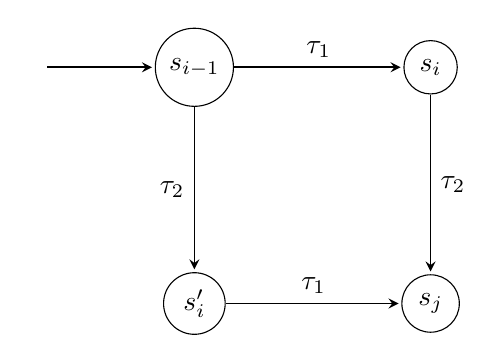
\begin{tikzpicture}
    [pre/.style={<-,shorten <=1pt,>=stealth,semithick}]
    \node (A) at (0,0) {};
    \node [shape=circle,draw=black] (B) at (2, 0) {\(s_{i-1}\)}
      edge [pre] node[above] {} (A);
    \node [shape=circle,draw=black] (C) at (2, -3) {\(s_i'\)}
      edge [pre] node[left] {\(\tau_2\)} (B);
    \node [shape=circle,draw=black] (D) at (5, 0) {\(s_i\)}
      edge [pre] node[above] {\(\tau_1\)} (B);
    \node [shape=circle,draw=black] (E) at (5, -3) {\(s_j\)}
      edge [pre] node[right] {\(\tau_2\)} (D)
      edge [pre] node[above] {\(\tau_1\)} (C);
  \end{tikzpicture}
  \caption{Influence of the order of independent transitions on the global state of an evaluation engine}
\label{fig:chap4:sec_run:exchange_transitions}
\end{figure}

\begin{lemma}[name = Duration of Enabledness]\label{lemma:enabled_till_scheduled}
  A node which is enabled stays enabled at least until it is scheduled.
  Formally: If a node \(n\) is enabled at step \(i\) in a run \(r\) it will stay enabled at least until the first step \(j > i\) with \(r(j) = (\tau,s), \mathit{node}(\tau) = n\).
  Note that it doesn't have to be disabled after step \(j\), because there could have been multiple events buffered on it's inputs.
\end{lemma}

\begin{proof}
  Let \(n\) be a node enabled at step \(i\) in a run \(r\).
  Let \((\tau_x,s_x) = r(x), x = i + 1\).
  If \(\mathit{node}(\tau_x) \neq n\), then the only influence that \(\tau_x\) can have on the node state \(\widetilde{n}\) of \(n\) is by appending produced events to one of the input queues, as per the definition of application of a transition.
  Since \(\tau_x\) can't remove events from the input queues in \(\widetilde{n}\) and on all input queues was at least one event buffered before the transition was applied, else \(n\) wouldn't have been enabled at step \(i\), \(\widetilde{n}\) will have at least as many input events buffered on every input as in the step before.
  This means that \(n\) is still enabled at step \(x\), and by induction at every later step until a transition with \(n\) as its node is taken.
\end{proof}

\begin{lemma}[name = Finiteness of Enabledness]\label{lemma:finiteness_enabledness}
  Whenever a node is enabled in a run, it can only be scheduled continously a limited number of times until becoming disabled.
\end{lemma}

\begin{proof}
  Let \(n\) be an enabled node at step \(i\) with the node state \(\widetilde{n}\).
  First let's assume that no parent of \(n\) are scheduled after step \(i\) and before \(n\) becomes disabled.
  Since the input queues of \(n\) are filled by previous transitions and only finite number of events are produced at every step, all of the queues can only have a finite number of events buffered at step \(i\).
  Since no parents of \(n\) are scheduled, the queues can't get fuller.
  Because all nodes represent functions, and all functions have to consume at least one input event (compare \Cref{sec:definitions:tessla_functions}), everytime \(n\) is scheduled at least one input queue of \(n\) will have one event less buffered after it performed its computation.
  Therefore the worst case is when \(n\) only consumes one event per computation.
  The maximum number of time \(n\) can be scheduled is therefore bounded by the sum of the number of events on all input queues at step \(i\).

  Now let's assume that also input nodes of \(n\) can be scheduled after step \(i\).
  Everytime an input node is scheduled it will add a finite amount of events to one input queue of \(n\).
  This leads to a cyclic behaviour: If an input queue can be scheduled infinitely often, infinite many events will be added to the input queue and \(n\) can possibly be scheduled infinitely often.
  If input queues can not compute infinitely often, only a finite amount of events are added to the inputs of \(n\) and therefore \(n\) can only be scheduled a limited number of times.
  Closer inspection of the nature of evaluation engines show why this is no problem: Only if the external trace fed to an evaluation engine is infinte the source nodes can compute infintely often.
  Hence for finite traces no node can compute infinitely often.
  Again the worst case is when \(n\) only consumes one event per computation.
  The number of times it can be scheduled is limited by the sum of the number of events buffered on the inputs at step \(i\) and the number of events that are produced by inputs of \(n\) after step \(i\).
\end{proof}

With the notion of runs and especially enabledness we can now define which schedules are seen as fair.

\begin{definition}[name = Fair Schedules]\label{def:fair_schedule}
  A schedule of an evaluation engine is called fair, if for all runs \(r\)  it produces the following holds:
  \begin{align*}
    &\forall i < \mathit{length}(r):\ &&\text{if }n\ \text{is enabled at step } i\\
    &                                 &&\text{then } \exists\, j \geq i\ \text{such that n is scheduled at step } j
\end{align*}
In other words, every enabled node is scheduled after a finite number of steps.
\end{definition}

Building on this we will investigate different fair schedules in the next chapter.

% !TEX root = ../thesis.tex
\chapter{Behaviours of Evaluation Engines}
\label{sec:behaviours}

Based on the definitions in \Cref{sec:definitions} we will now look at different schedules of evaluation engines and compare them.
This is done in multiple steps: starting with a small subset of allowed schedules and functions and iteratively adding more complex cases.

For the comparision we will use timed transducers from \Cref{sec:definitions:timed_transducer}.
To do this the notion of a run of an evaluation engine is not sufficient: transducers describe a relationship between inputs and outputs, runs describe stepwise generation of internal and output events.
Therefore the \emph{behaviour} of a run is defined, which maps a run to relationship between inputs and outputs.

\begin{definition}[name = Behaviour of a Run]\label{def:behaviour_run}
  Let \(r\) be a run of an evaluation engine.
  The behaviour \(\beta_r\) of it is a timed transducer: A set of tuples of timed sequences.
  It is calculated as follows:
  \begin{enumerate}
    \item Let \(\beta_r = \emptyset\) and \(r_p\) an empty prefix of \(r\).
    \item Remove the prefix  from \(r\), where the first transition consumes an input upto but not including the next transition where an input is consumed, and append it to \(r_p\).
    \item Select the sequence of all output events \(O_p\) (which is possible empty) that are produced at any step in \(r_p\).
    \item Select the sequence of all input events \(E_p\) that are consumed at any step in \(r_p\).
    \item Add the tuple \((E_p,O_p)\) to \(\beta_r\).
    \item Goto step 2 if \(r\) is not empty, else terminate.
  \end{enumerate}

  Stated simple the run is chopped into pieces, where each piece begins with the consumption of an input events and ends before the next input is consumed.
  The pieces are then merged from left to right: First take all inputs and outputs consumed and produced upto the current piece and add them to the behaviour, then merge the current piece with the next and repeat.
\end{definition}

\begin{exmp}[name = Construction of a Behaviour]\label{exmp:construction_of_behaviour}
  In \Cref{table:chap5:sec_behaviour:construction_run} it is shown how a behaviour is built from a run.
  The run ist denoted only by its transitions, events are labeled based on their type: \(e_i\) are external (read: input) events, \(i_i\) are internal events and \(o_i\) are output events.
  Parts of the run in the same color are the transitions that end up in the same piece when applying the constuction algorithm.
  The tuples show how the sequence of input and output events from the pieces are extracted.
  The behaviour of the run is the set of the tuples.

  \begin{table}
    \renewcommand{\arraystretch}{1.5}
    \begin{tabular}{llllll}
      Run    & \multicolumn{5}{l}{\textcolor{thesisred}{\(    (\{e_1\},\{i_1\})\ (\{i_1\},\{i_2\})\ (\{i_1,i_2\},\{o_1\})\ \)}\textcolor{thesisblue}{\((\{e_2\},\{i_3\})\ (\{i_2,i_3\},\{o_2\})\)}\(\hookleftarrow\)} \\
             & \multicolumn{5}{l}{\hspace{1em}\textcolor{thesisblue}{\(    (\{i_3\},\{o_3\})\ \)}\textcolor{thesisgreen}{\((\{e_3\},\{i_4\})\ \)}\textcolor{thesisyellow}{\((\{e_4\},\{i_5\})\ (\{i_4,i_5\},\{o_4\})\)}} \\
      Tuples & \textcolor{red}{\((e_1,o_1)\)} & \textcolor{thesisblue}{\((e_1e_2,o_1o_2o_3)\)} & \textcolor{thesisgreen}{\((e_1e_2e_3,o_1o_2o_3)\)} & \textcolor{thesisyellow}{\((e_1e_2e_3e_4,o_1o_2o_3o_4)\)} \\
    \end{tabular}
    \caption{Example how the behaviour of a run is constructed}\label{table:chap5:sec_behaviour:construction_run}
  \end{table}
\end{exmp}

The behaviour of a run is a timed transducer since all events have timestamps and all consumed events are strictly ordered by their timestamp, since inputs to an evaluation engine are required to be ordered by their timestamp.

Since the behaviour encodes the relationship between inputs and outputs a run produces it provides the foundation to reason about equivalence between different runs and whole evaluation engines.

\begin{definition}[name=Equivalence of Runs]\label{def:equivalence_runs}
  Two runs are called equivalent if their behaviour is observational equivalent.
\end{definition}

Now we can define when two evaluation engines are called equivalent based on their runs

\begin{definition}[name=Equivalence of Evaluation Engines]\label{def:equivalence_eval_engine}
  Two evaluation engines are called equivalent, if for every run that one can produce there is an observational equivalent run in the other.
\end{definition}

\section{Schedules Without Timing Functions}
\label{sec:behaviours:without_timing}

For a first step we specify and compare behaviours of different approaches to evaluate \gls{tessla} specifications without timing functions.
Without timing functions all nodes work only on values or the presence of events and will emit exactly one event at every computation, either a normal or a progress event.
This leads to behaviours that can be easily reason about, as seen in the next sections.

All systems to evaluate \gls{tessla} specifications we will look at are based on the described structure in \Cref{sec:definitions:eval_engine}.
While there are other approaches to evaluation, a \gls{dag} based approach seems to fit most naturaly and focusing on one structure makes comparing systems easier.

Let's recap and summarize how an evaluation engine performs its computation.
Each evaluation engine will work in steps, where each step is synonymous with an index in the run of the system.
Therefore at each step one enabled node is scheduled to perform its operation, represented as the transition in the run.
The transition will encode one of the following three things that can happen:

\begin{itemize}
  \item The next external event (external events have to be totally ordered by their timestamp) can be consumed by a source in the \gls{dag}, which generates internal events, that are propagated to its children.
  \item An internal node, which has at least one new input buffered on all of its input queues, can perform its computation and generate a new internal event, which is propagated to the children of that node.
  \item An output node, which has at least one new input buffered on all of its input queues, can produce a new output.
\end{itemize}

Evaluation engines are free in the way they are scheduling their nodes, only limited by causality (no event can be consumed before it's produced), which is guaranteed by the enabledness criteria.
In the following evaluation engines are classified by their scheduling approaches.

\subsection{Greedy Evaluation Engines}
\label{sec:behaviours:without_timing:greedy}

The first class of evaluation engines are called greedy.

\begin{definition}[name = Greedy schedule]\label{def:greedy_schedule}
  A schedule of an evaluation engine built by the following steps is called \emph{greedy}.
  \begin{enumerate}
    \item Select all nodes that are no sources, let their count be \(i\)
    \item Label them with unique natural numbers from \([1,i]\) in reverse topological order
    \item Label the remaining nodes with unique natural numbers bigger than \(i\)
    \item Schedule the enabled node with the lowest label first
  \end{enumerate}

  We also call an evaluation engine greedy if we mean it's run with a greedy schedule.
\end{definition}

Obviously for many \glspl{dag} there is no unique reverse topological order, therefore one can be chosen by the evaluation engine.
We will show in \Cref{sec:behaviours:equivalence_without_timing:greedy} that all topological orders will produce observational equivalent behaviours.

The greedy schedule ensures that no node is scheduled which has a successor that can be scheduled, therefore events are \emph{pushed} through the \gls{dag} towards an output node as fast as possible.
As shown in \Cref{sec:behaviours:without_timing:greedy:is_fair} any schedule built like this is fair.

Greedy evaluation engines offer a good start to reason about behaviours and will be used as a comparision for all other evaluation engines.

\begin{definition}[name = Valid Evaluation Engines]\label{def:valid_eval_engine}
  An evaluation engine is called \emph{valid} if it is equivalent to a greedy evaluation engine.
\end{definition}


\begin{figure}
  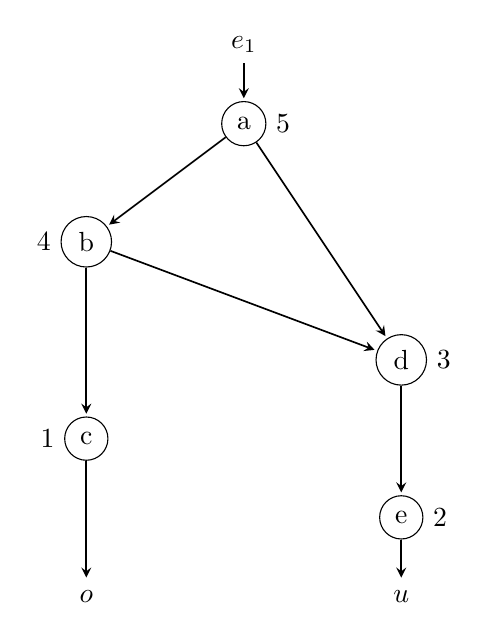
\begin{tikzpicture}
    [pre/.style={<-,shorten <=1pt,>=stealth,semithick}]
    \node (s) at (2,5) {\(e_1\)};
    \node [shape=circle,draw=black] (a) [label=right:5] at (2, 4) {a}
      edge [pre] (s);
    \node [shape=circle,draw=black] (b) [label=left:4] at (0,2.5) {b}
      edge [pre] (a);
    \node [shape=circle,draw=black] (c) [label=left:1] at (0,0) {c}
      edge [pre] (b);
    \node [shape=circle,draw=black] (d) [label=right:3] at (4,1) {d}
      edge [pre] (a)
      edge [pre] (b);
    \node [shape=circle,draw=black] (e) [label=right:2] at (4,-1) {e}
      edge [pre] (d);
    \node (o1) at (0,-2) {\(o\)} edge [pre] (c);
    \node (o2) at (4,-2) {\(u\)} edge [pre] (e);
  \end{tikzpicture}
  \hspace{20mm}
  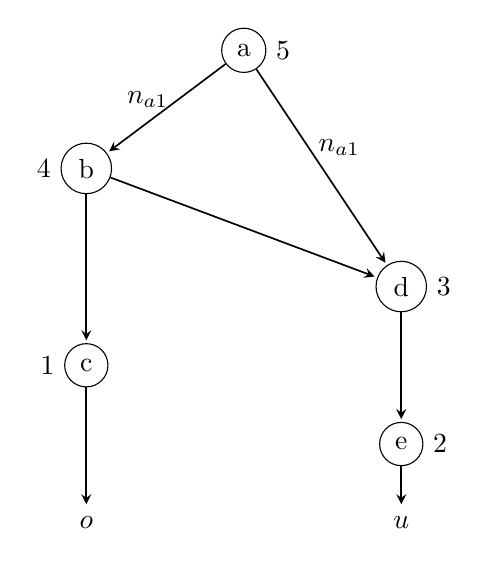
\begin{tikzpicture}
    [pre/.style={<-,shorten <=1pt,>=stealth,semithick}]
    \node [shape=circle,draw=black] (a) [label=right:5] at (2, 4) {a};
    \node [shape=circle,draw=black] (b) [label=left:4] at (0,2.5) {b}
      edge [pre] node[align=left,left,pos=0.6] {\(n_{a1}\)} (a);
    \node [shape=circle,draw=black] (c) [label=left:1] at (0,0) {c}
      edge [pre] (b);
    \node [shape=circle,draw=black] (d) [label=right:3] at (4,1) {d}
      edge [pre] node[align=right,right,pos=0.6] {\(n_{a1}\)} (a)
      edge [pre] (b);
    \node [shape=circle,draw=black] (e) [label=right:2] at (4,-1) {e}
      edge [pre] (d);
    \node (o1) at (0,-2) {\(o\)} edge [pre] (c);
    \node (o2) at (4,-2) {\(u\)} edge [pre] (e);
  \end{tikzpicture}
  \caption[Visualization of a simple evaluation engine with a greedy schedule.]{Visualization of a simple evaluation engine with a greedy schedule. The left side shows the initial state of the evaluation engine with one input event that can be consumed. The right side shows the state after the input event was consumed and now two internal events are send to the children of the input node.}
  \label{fig:chap5:sec_greedy:visual_dag}
\end{figure}

\Cref{fig:chap5:sec_greedy:visual_dag} visualizes a greedy evaluation engine.
It shows two \glspl{dag} representations of an evaluation engine  where the nodes \(a\) to \(e\) are labeled in a reversed topological order and \(o\) and \(u\) represents two output streams.
The left system is in its initial state and an input event \(e_1\) is present and can be consumed by the input node \(a\).
When a node is chosen to compute by the scheduler, only node \(a\) is enabled, therefore it is scheduled.
The right system is the representation of the next step: node \(a\) has consumed the external event and produced an internal event \(n_{a1}\), which is propagated to all its children: nodes \(b\) and \(d\).
In the next step node, \(b\) would be scheduled, because it has the lowest number of any node that can compute (actually it's the only node that can compute at all, because \(d\) has to wait for the event from \(b\)).
After \(b\) is scheduled, it would produce the internal event \(n_{b1}\) which would then be distributed to nodes \(c\) and \(d\).

The complete run of the greedy engine for one input is the following, where the states are omitted:

\begin{align*}
  \langle
    (\lambda,                             s_0),
    ((\{ n_{a1}         \}, \{n_{b1}\}),  s_1),
    ((\{ n_{b1}         \}, \{o_1\}),     s_2),\\
    ((\{ n_{a1}, n_{b1} \}, \{n_{d1}\}),  s_3),
    ((\{ n_{d1}         \}, \{u_1\}),     s_4)
  \rangle
\end{align*}

If there were more than one input event, at this point node \(a\) would be scheduled again.
It would consume the next external event and the following nodes would be scheduled in the same order as before, extending the run in an obvious way.

\subsubsection{Fairness of Greedy Schedules}
\label{sec:behaviours:without_timing:greedy:is_fair}

It remains to show that greedy schedules are fair.

\begin{lemma}[name = Greedy Schedules are Fair]\label{lemma:greedy_schedules_are_fair}
  Any greedy schedule is fair.
\end{lemma}

\begin{proof}
  Let \(a\) be a node with the label \(n\), which is enabled at step \(i\) and is no source.
  Because evaluation engines can only contain a finite number of nodes there can only be a finite number of enabled nodes with a smaller label than \(n\).
  Because of \Cref{lemma:finiteness_enabledness}, all nodes with a smaller label than \(n\) will become disabled after a finite number of steps.
  Let that number be \(j\).
  The only way new events could enter the system are through sources, but they have bigger labels than \(n\), as by the definition of the schedule, and therefore can't be scheduled before \(n\).
  Because of \Cref{lemma:enabled_till_scheduled}, \(a\) will still be enabled after these steps.
  So \(a\) is the enabled node with the lowest label at step \(i + j\) and therefore will be scheduled.

  Now let \(a\) be a source.
  Sources are only scheduled when no internal node is enabled since they are labeled with higher numbers than all internal nodes.
  Based on the same reasoning as in the first case at some point all internal nodes will become disabled, therefore a source node has to be scheduled.
  This source can either be \(a\) or another source, recall that only one source is enabled at any time because of the environment of an evluation engine.
  If another source was scheduled, after a finite amount of steps all internal nodes will have to become disabled again.
  Since finite traces are evaluated at some point either the trace will end without ever feeding an input to \(a\), then \(a\) will never be enabled, or at some point \(a\) will receive an external event.
  When \(a\) receives an external event, it will be the only enabled source, else no input would be fed to an input at that step.
  Therefore \(a\) will be scheduled the next time no internal nodes are enabled.
\end{proof}


\subsection{Fair Evaluation Engines}
\label{sec:behaviours:behaviour_without_timing:fair}

Obviously greedy schedules are only a small subset of all fair schedules.
As the next step we will look at the rest of them.

\begin{definition}[name = Fair Evaluation Engines]\label{def:fair_evaluation_engines}
  A fair evaluation engine is one with a fair schedule.
\end{definition}

In contrast to a greedy evaluation engine a fair one has no fixed schedule, meaning that at each step any enabled node can be scheduled.
Therefore predecessors of enabled nodes can perform multiple computations before their children are scheduled and events are not \emph{pushed} through the \gls{dag} as fast as possible.

The difference between greedy and fair schedules are similar to the ones of synchronous and asynchronous transducers: A greedy schedule will ensure that outputs are produced as fast as possible while a fair can \emph{delay} the outputs by consuming multiple inputs first and scheduling internal nodes multiple times before scheduling an output node.
But note that there is an important difference between synchronous transducers and the behaviour of a greedy evaluation engine: A greedy evaluation engine can produce multiple events at every step.

\section{Equivalence of Different Schedules Without Timing Functions}
\label{sec:behaviours:equivalence_without_timing}

The behaviour of a run of an evaluation engine with a given schedule allows us to reason about equivalence.

As by \Cref{def:valid_eval_engine} any evaluation engine has to be equivalent to a greedy one to be valid.

The equivalence is shown in two steps: first in \Cref{sec:behaviours:without_timing:greedy} it is shown, that all possible greedy engines for a specification are equivalent, so there is only one valid evaluation for a specification over a fixed input.
Afterwards in \Cref{sec:behaviours:equivalence_without_timing:greedy_fair} it is shown that any fair evaluation engine is equivalent to a greedy one.


\subsection{Equivalence of Greedy Systems}
\label{sec:behaviours:equivalence_without_timing:greedy}

When given a series of input events, two greedy evaluation engines for a specification with different schedules will have different runs.
But both will produce all outputs that can be produced after consuming one specific input before the next input is consumed as reasoned in \Cref{sec:behaviours:without_timing:greedy}.
Also both runs will obviously have the same length (both engines are the same \gls{dag}, so they have the same number of nodes), let that length be \(l\).

To proof the equivalence of both engines we can prove the equivalence of their runs.
To show the equivalence it is shown that two runs \(r_1\) and \(r_2\) of two evaluation engines based on the same graph but with a different greedy schedule can always be reordered to become closer while preserving observational equivalence.
If such a closer run always exist, we will show that the run with closeness \((l, 0)\) to \(r_1\), which has to be \(r_1\) itself, is also observational equivalent to \(r_2\).

\begin{theorem}[name = Equivalence of Different Greedy Evaluation Engines]\label{theorem:equivalence_greedy_eval_engines}
  Two greedy evaluation engines for a specification with different schedules are equivalent.
\end{theorem}


\begin{proof}\label{proof:equiv_greedy_engines}
  Let \(r_1, r_2\) be the runs of two greedy evaluation engines for the same specification which received the same inputs.
  Because each \gls{tessla} specification contains only a finite amount of functions and works on finite traces, the runs also have to be finite.

  If the two runs aren't equal, they must have a closeness which is smaller than \((l, 0)\).
  Let \([r_2]\) be the set of all runs that are observational equivalent to \(r_2\).
  If \(r_1\) is in this set, we would be done.
  Let's assume that \(r_1\) is not in the set.
  Therefore all runs in the set have to have a smaller closeness than \((l,0)\) to \(r_1\), since the only run with a closeness of \((l,0)\) to another run is the run itself.
  Select one run \(r_2' \in [r_2]\) which has the biggest closeness to \(r_1\).
  Let \((d,k) = \delta(r_1, r_2')\).

  This means that at step \(d\) the run \(r_2'\) has taken a different transition than run \(r_1\).
  Let the transitions the runs have taken be \(\tau_1\) for \(r_1\) and \(\tau_2\) for \(r_2'\).
  Run \(r_2'\) will take transition \(\tau_1\) at step \(d+k\) (as per the definition of the closeness).
  Obviously the two transitions have to be independent of each other, else they couldn't have been taken in different order by the two runs.

  If \(k > 1\) there will be a transition \(\tau_2' \neq \tau_1\) which is taken by the run \(r_2'\) at step \(d+(k-1)\).
  While this transition \(\tau_2'\) must also be taken in the first run as per \Cref{lemma:enabled_till_scheduled}, it's not possible, that it was taken before \(\tau_1\), beause then the two runs wouldn't have been the same upto the point where \(\tau_1\) was taken.
  Therefore \(\tau_1\) has to be independent of \(\tau_2'\), and because \(\tau_2'\) was scheduled by the second run before \(\tau_1\) both transitions are independent of each other.

  As of \Cref{lemma:exchange_independent_transitions} which one of them is taken first won't change the rest of the run at all after both transitions were applied and the run stays valid.
  Therefore there is a valid run \(r_2''\), which is equal to \(r_2'\), except that the transitions \(\tau_1, \tau_2'\) are scheduled the other way around.
  See \Cref{fig:chap5:sec_greedy:maximize_closeness} for a visualization of the runs.
  Dotted edges represent multiple transitions. The visualization shows how the three runs \emph{branch} and \emph{merge} after certain steps.
  The run \(r_1\) is marked in red, \(r_2''\) in green and \(r_2'\) in blue.
  As you can see the run \(r_2''\) has a bigger closeness to \(r_1\) since it takes \(\tau_1\) before \(\tau_2'\).
  Note that \(r_1\) is only known upto step \(d\), especially the transitions \(\tau_2, \tau_2'\) will be taken eventually, but it isn't known when or in which order.

  \begin{figure}
    \centering
    \colorlet{path1}{thesisred}
    \colorlet{path2}{thesisgreen}
    \colorlet{path3}{thesisblue}
    \begin{tikzpicture}[->,>=stealth',shorten >=1pt,auto,node distance=2.8cm, semithick]
      \tikzstyle{every state}=[text=black,minimum width=1.5cm]

      \node[state] (A)                   {$s_0$};
      \node[state] (B) [below of=A] {$s_{d-1}$};
      \node[state] (C) [below left of=B] {$s_d$};
      \node[state] (D) [below right of=B] {$s'_d$};
      \node[state] (E) [below of=D] {$s'_{d+k-2}$};
      \node[state] (F) [below left of=E] {$s''_{d+k-1}$};
      \node[state] (G) [below right of=E] {$s'_{d+k-1}$};
      \node[state] (H) [below right of=F] {$s'_{d+k}$};
      \node[state, draw=none, fill=none, below of=H] (X) {};

      \path (A.260) edge [path1, dashed]  node {} (B.100)
        (A.270) edge [path2, dashed] node {} (B.90)
        (A.280) edge [path3, dashed] node {} (B.80)
        (B)   edge [above left, path1]  node {$\tau_1$} (C)
        (B.320) edge [path3]  node {$\tau_2$} (D.130)
        (B.310) edge [path2]  node {} (D.140)
        (D.265) edge [path2, dashed] node {} (E.95)
        (D.275) edge [path3, dashed] node {} (E.85)
        (E) edge [path2, above left] node {$\tau_1$} (F)
        (E) edge [path3] node {$\tau'_2$} (G)
        (G) edge [path3, below right] node {$\tau_1$} (H)
        (F) edge [path2, below left] node {$\tau'_2$} (H)
        (C) edge [path1, dashed] node {$\tau_2$} node [pos=0.8, left] {$\tau'_2$} ($(C |- X) + (0, 0.75cm) $)
        (H.265) edge [path2, dashed] node {} (X.95)
        (H.275) edge [path3, dashed] node {} (X.85);
    \end{tikzpicture}
    \caption[Visualization of three runs of an evaluation engine]{Visualization of three runs of an evaluation engine. The left run differs from the two right runs after state \(s_{d-1}\) while the two right runs only differ by the order of the transitions \(\tau_1\) and \(\tau'_2\).}
    \label{fig:chap5:sec_greedy:maximize_closeness}
  \end{figure}

  When two adjacent transitions are exchaned besically two things can happen:

  \begin{itemize}
    \item Outputs can be produced later, maybe moving them to the next piece in the contsruction of a behaviour (this happen when a transition producing outputs is exchanged with the next transition which consumes an external event)
    \item Outputs can be produced earlier, which can move them to an earlier piece in the construction of the behaviour (this happens in the opposite case, where a transition consuming an external event is pushed before one that produces outputs)
  \end{itemize}

  While the order of outputs in the tuples of the behaviour will change when two transitions producing outputs are exchanged, observational equivalence isn't influenced, since it is defined over reordered outputs.

  Let's test if \(r_2''\) is observational equivalent to \(r_2'\):
  We will compare how the behaviour of the run \(r_2'\) changes when the transition \(\tau_1\) is exchanged with \(\tau_2'\).
  The comparision is based on the different cases the transitions can encode.
  Some of the cases are not feasible, they are listed for the sake of completeness and to explain why they can't happen.
  The cases are:

  \begin{enumerate}
    \item No inputs are consumed and no outputs produced by either transition. This obviously won't change the behaviour at all.
    \item \(\tau_2'\) consumes an input and doesn't produce an output and
      \begin{enumerate}
        \item \(\tau_1\) doesn't consume an input and doesn't produce an output. This won't change the behaviour, since \(\tau_1\) didn't added anything to it in the first place.
        \item\label{sec:behaviours:without_timing:greedy:non_greedy_1} \(\tau_1\) doesn't consume an input, but produces one or more outputs. This changes the behaviour, since \(\tau_1\) is now part of the piece starting before \(\tau_2'\). Therefore the produced outputs are now part of one more tuple of the behaviour. But note that it still is part of all tuples built from the later pieces of the run. Therefore the two behaviours are still observational equivalent: All tuples in the behaviour are still the same, except that one or more output events are produced one step earlier, which doesn't hurt observational equivalence.
        \item\label{sec:behaviours:without_timing:greedy:impossible_case} \(\tau_1\) consumes an input but doesn't produce an output. This case can't happen, since inputs to evaluation engines are totally ordered by their timestamp and therefore \(\tau_2'\) couldn't have been scheduled after \(\tau_1\) in \(r_1\) and before \(\tau_1\) in \(r_2\).
        \item \(\tau_1\) consumes an input and produces outputs. This case can't happen for the same reason.
      \end{enumerate}
    \item \(\tau_2'\) produces one or more outputs and doesn't consume an input and
      \begin{enumerate}
        \item \(\tau_1\) doesn't consume an input and doesn't produce an output. This won't change the behaviour, since \(\tau_1\) didn't added anything to it in the first place.
        \item \(\tau_1\) doesn't consume an input, but produces one or more outputs. This only changes the order of the output events in the behaviour, but since they are reordered by their timestamp and the order of events with the same timestamp isn't important for observational equivalence, the new run is still observational equivalent.
        \item \(\tau_1\) consumes an input but doesn't produce an output. This will \emph{delay} the production of the outputs from \(\tau_2'\) by one piece of the chopped run. While this changes the behaviour it preserves observational equivalence.
        \item \(\tau_1\) consumes an input and produces outputs. This is kind of a combination of the previous two cases. The outputs from \(\tau_2'\) are \emph{delayed} by one piece and the outputs of \(\tau_1\) are now produced before them. But still all outputs are produced, only in different order and maybe one step later. Therefore observational equivalence holds. Also note that such a transition isn't very useful as argued in the next case.
      \end{enumerate}
    \item \(\tau_2'\) produces one or more outputs and consumes an input. First of all note that this is a rather made up combination that can only happen when a source is an output node at the same time and therefore doesn't have much of a purpose. But for the sake of completeness let's look at the cases following from this:
      \begin{enumerate}
        \item \(\tau_1\) doesn't consume an input and doesn't produce an output. Again won't change the behaviour, as in earlier cases.
        \item\label{sec:behaviours:without_timing:greedy:non_greedy_2} \(\tau_1\) doesn't consume an input, but produces one or more outputs. Preserves observational equivalence since the outputs of \(\tau_1\) are only produced one step earlier than before.
        \item \(\tau_1\) consumes an input. This case can't happen as reasoned in \Cref{sec:behaviours:without_timing:greedy:impossible_case}.
      \end{enumerate}
  \end{enumerate}

  So for all cases that can happen, the run which is obtained by exchanging the two adjacent transitions is observational equivalent to the run without the change.
  The exchange of the two transitions brings the closeness of the new run by construction one step closer to \(r_1\).
  This means, since observational equivalence is transitive, that there is an observational equivalent run to \(r_2\), the run \(r_2''\),  which has at least the closeness \((d, 1)\).

  If \(k = 1\) the transition \(\tau_2'\) from the previous case is equal to \(\tau_2\).
  The reasoning for all cases stays exactly the same, in the end we will obtain a run \(r_2''\) which is observational equivalent to \(r_2'\) but has the closeness \((d, 0)\) to \(r_1\).
  This obviously doesn't make sense: The first element of the closeness is the last step where both runs are equal, the second element describes how many steps afterwards the differing transition was taken.
  But if it was taken right in the step after the last equal step, there is no difference at that position, so the closeness of \(r_1\) and \(r_2''\) can be at least \((d+1, x), x \in \mathbb{N}_{>0}\).
  This also contradicts our initial statement that \(r_2'\) was the run with the biggest closeness to \(r_1\) which is observational equivalent to \(r_2\).

  Combined we can now say, that there is no upper bound on the closeness of observational equivalent runs of \(r_2\) to \(r_1\), therefore the run with the closeness \((l, 0)\) also has to be equivalent to \(r_2\).
  And as already stated, only the run \(r_1\) can have the closeness of \((l, 0)\) to \(r_1\).
  Therefore \(r_1\) has to be observational equivalent to \(r_2\).
\end{proof}


This characteristic of greedy schedules gives us a baseline to compare other schedules to.
Since all greedy schedules of an evaluation engine produce observational equivalent behaviours we can choose any run produced by such a schedule and compare any other run to it.
In the next section we will do this for all fair schedules.

\subsection{Equivalence of Greedy and Fair Evaluation Engines}
\label{sec:behaviours:equivalence_without_timing:greedy_fair}

Let's recap what fairness of a schedule means: Whenever a node becomes enabled in a run it has to be scheduled eventually.
What makes fair schedules harder to reason about than greedy ones is that for one they don't have to be deterministic and furthermore that it's possible that an enabled node is not scheduled for a very long time.

Before reasoning about equivalence of greedy and fair schedules let's look at a kind of fair schedule that can be seen as worst case.
Basically it is the reverse of a greedy schedule: Always schedule the enabled node that is closest to a source.
Note that this schedule is not fair for infinite input traces.
Stated simple this schedule will consume all input events and produce all output events per \emph{level} of the \gls{dag}, starting at the sources and moving towards the outputs.
The behaviours of runs with such a schedule are pretty special: Since no output is produced before all external events are consumed (except if a source is also an output) only one tuple of the behaviour will contain any outputs, to be specific the one which contains the sequence of all inputs as the first element.
An abbreviated example of such a run is \((e_1,())\ (e_1e_2,())\ (e_1e_2e_3,())\ (e_1e_2e_3e_4,o_1o_2o_3o_4o_5)\).
Such a run needs obviously more reordering than a greedy one to become observational equivalent to another greedy one since greedy schedules try to produce outputs as early as possible.

This example shows what the difference is when reordering a fair run in contrast to a greedy run: basically more transitions have to be reordered since outputs can be produced later.

Let's revisit the cases from \Cref{proof:equiv_greedy_engines}:
Actually the \Cref{sec:behaviours:without_timing:greedy:non_greedy_1,sec:behaviours:without_timing:greedy:non_greedy_2} can't happen for greedy runs.
If in a run \(r_1\) a transition \(\tau_1\), which produces an output, has to be exchanged with an earlier transition \(\tau_2\), that consumed an external event, to become closer to a greedy run \(r_2\), \(r_1\) couldn't have been greedy in the first place:
Greedy schedules ensure by construction that all outputs that can be produced based on consumed external events are produced before the next external event is consumed.
If \(\tau_1\) happened before \(\tau_2\) in a greedy run, the outputs from \(\tau_1\) can be produced without consuming the external event from \(\tau_2\) before, hence a run in which \(\tau_2\) happens before \(\tau_1\) couldn't be produced by a greedy schedule.

It's noteworthy that actually the whole proof of \Cref{theorem:equivalence_greedy_eval_engines} doesn't depend on the fact, that the runs are produced by greedy schedules.
The only real requirement is fairness, meaning that all transitions that can happen will eventually happen.
Therefore the proof does hold without change for \Cref{theorem:equivalence_greedy_fair_engines}.

\begin{theorem}[name = Equivalence of Fair and Greedy Evaluation Engines]\label{theorem:equivalence_greedy_fair_engines}
  Any fair evaluation engine is equivalent to a greedy evaluation engine for the same specification.
\end{theorem}

\section{Timing functions}
\label{sec:behaviours:timing_functions}

As stated before timing functions add complexity.
But, as we will see, the reasoning from previous sections still hold for evaluation engines which include timing functions.
The two characteristics of timing functions are, that they can produce events with timestamps that is not equal to the timestamp of any input event and that they can produce multiple output events for every input event.

The proof for equivalence of asynchronous evaluation engines does not depend on the fact, that events only carry timestamps that are present on input events.
Therefore this characteristic of timing functions doesn't interfere with our theory.

That a timing function can generate multiple outputs for input is more critical.
The proof requires that evaluation engines terminate eventually when the input trace is finite.
If each node of an evaluation engine can only generate at most one event per input, the number of total events that can be produced is bound by the size of the input trace, the number of nodes and the number of edges of the evaluation engine.
If a timing function is allowed to generate infinitely many outputs for an input the evaluation engine would never terminate.
For now we choose to not allow such a function.

For future work we like to note that the fact that we only consider fair schedules which will schedule each enabled node eventually.
Therefore even timing functions which generate infinite many events cannot produce a lifelock in an evaluation engine.

% !TEX root = ../thesis.tex
%
\chapter{Implementation Details}
\label{sec:implementation}

Besides the theoretical basics presented in \Cref{sec:related} the \gls{tessla} runtime of this thesis is built upon a number of technologies.
To better understand the decisions made during the implementation this chapter will give an overview of these decisions and show why they were choosen.

As already mentioned, the implemented runtime itself is independent on the way traces are generated.
Therefore we will not only look at the building blocks for the runtime itself but also examine related projects which can be used to obtain traces, which then can be monitored by the runtime.
Because the format of the traces can differ heavily, depending on how and why they were collected, they are not only used to test the runtime but also to determine how the runtime can consume them.

\section{TesslaServer}
\label{sec:implementation:tesslaserver}

The runtime that evaluates specifications against traces is implemented in the programming language Elixir, which itself is built on top of Erlang, the \gls{beam} \gls{vm} and \gls{otp}.
To understand why this platform was choosen we will look at the Erlang ecosystem in the next section.
Note that in the following sections terminology from \Cref{sec:related,sec:definitions} as well as from Erlang and Elixir is extensively used.

\subsection{Erlang and Elixir}
\label{sec:implementation:tesslaserver:erlang_elixir}

Erlang was originally developed 1987 as a language to program systems with limited resources which had to be highly fault tolerant.
The primary purpose of the language were phone switches, which have to handle large amounts of connections at the same time.
Since the switches were not deployed at a central location but wherever they are needed crashes would entail long downtimes of the system.
Also, since customers expect permanent service, the platform had to provide a way to update the software without downtimes.
Erlang and the \gls{otp} platform are built on top of these requirements.

While the requirements of TesslaServer are quite different we will see that the Erlang platform is a great fit for the implementation.

The rather new programming language Elixir\footnote{\url{http://elixir-lang.org}} can be seen as a dialect of Erlang.
Elixir code is compiled into bytecode for \gls{beam} and can therefore interoperate with Erlang code.
The rationale to use Elixir instead of Erlang directly is twofold:
On the one hand Erlangs syntax is pretty different from that of most modern general purpose programming languages while Elixirs syntax was developed based on modern language design principles.
Also, Elixir supports metaprogramming, meaning you can write code that generates code at compile time, a feature we use heavily, as described in \Cref{sec:implementation:tesslaserver:architecture}.

One of the core strengths of the Erlang platform is it support to exploit multiple processor cores, even if these cores are deployed over multiple machines in a network.
The platform offers tools to develop code that can be distributed over multiple processors.
This distribution is transparent to the developer.
The underlying concept of the distribution is the actor model, first introduced in \cite{Hewitt1973}.

An actor is basically a self contained entity, that holds a state and can receive and send messages to other actors.
Since an actor manages its own state and is the only one that can manipulate it, an actor can be scheduled on any core as long as the runtime guarantees transparent message delivery.
When an actor receives a message from another actor the \gls{beam} \gls{vm} will eventually schedule the code responsible for handling the message on an available core.
This code can then access the state, alter it and send a response to the sender of the message or send messages to other actors.
In this sense an actor can be seen as a state machine, which alters its state everytime it receives a message.
Since actors are independent of each other they can be scheduled in parallel on multiple processors.
Only when two actors synchronously communicate one actor has to wait for the other.

Another reason to choose the Erlang platform was its support for multiple platforms, including resource contrained ones.
While this thesis only considers offline monitoring it may be a future goal to perform online monitoring with TesslaServer.
To enable this feature the runtime has to be able to run on the same hardware architecture as the monitored program sharing resources.
An example of the variety of the supported platforms of Erlang and Elixir is the Nerves project\footnote{\url{http://nerves-project.org}} which allows developers to build embedded software.

\subsection{Architecture}
\label{sec:implementation:tesslaserver:architecture}

As described in \Cref{sec:definitions:eval_engine} \gls{tessla} specifications form a \gls{dag} of nodes, which perform transformations on streams and send their computed streams to children nodes.
Streams can be seen as a sequence of events or changes that can be represented as messages between the nodes.
This form of specification can be easily implemented as an actor based system, where each vertex in the \gls{dag} is implemented as an actor and the communication between adjacent vertices is realised with message passing between the corresponding actors.
Interestingly, as we will see in the following, this architecture enables the enforcement of greedy schedules, which are described in \Cref{def:greedy_schedule}, while the Erlang runtime itself only guarantees a fair scheduling.
To understand how a greedy schedule can be enforced we have to look at the internals of message passing and handling in Erlang and Elixir.

Basically there are two ways two Erlang processes can communicate with each other through messages: synchronous and asynchronous.
The \emph{call} \gls{api} is used too send a message synchronously.
A \emph{call} will send a message to another process and block until a response is received.
The \emph{cast} \gls{api} is the asynchronous counterpart, which will send a message and immediately passes back control to the process that used it.

As can be easily seen the usage of the synchronous \gls{api} will lead to a valid greedy schedule, since the sources in the \gls{dag} will have to wait for their children to finish and the children will transitively have to wait for their children.
This means that each new message gets distributed through the whole graph as fast as possible.
While this behaviour is an interesting observation the actual implementation uses the asynchronous \gls{api} to take better advantage of parallel evaluation.

An important characteristic of \gls{tessla} specifications is that they can specify properties targeting realtime characteristics.
On one hand this enables specifications that are not feasible with more classical specification approaches, like \gls{ltl} or \gls{lola}, which work on synchronous streams.
On the other hand it adds complexity to monitoring approaches, since it adds asynchronicity to all parts of the system.
One point where this is important is in the way systems have to be monitored, or more precisely how their generated events are encoded.
For synchronous monitoring approaches, encoding the fact that an event happened is sufficient.
However for asynchronous ones it is important to know at which exact time each event happened.
For an implementation of an asynchronous monitoring approach this simply means, that the representation of events has to include information about the time at which the event happened.
Another consequence of the asynchronous nature is discussed in \Cref{sec:implementation:tesslaserver:nodes} with the notion of the \emph{front} of events.

\subsection{Synthesis of the Evaluation Engine}

The first step that TesslaServer has to perform to evaluate a specification is to synthesize the evaluation engine that will consume event traces and perform the corresponding computation.
For this step a specification is compiled into a \gls{json} based format that describes the nodes and their relationship.
\Cref{listing:spec_json} shows a minimal example of the format, which includes three nodes: two literals and a node adding their value.

\lstinputlisting[float,language=json,caption={Minimal example of the \gls{json} based specification format. The specification describes a \gls{dag} with three nodes: two literals as the sources and an adder as their child.},label=listing:spec_json]{content/code/minimal.tessla}

The compiler performs multiple checks, including type checks and ensures that no loops are present in the specification, and transformations, namely resolve macros and other syntactic elements of the specification language.
Since the compiler acts as a safety guard, TesslaServer assumes that a given specification is error free and performs no redundant safety checks.
Invalid specifications can therefore lead to all kinds of wrong behaviour if fed to TesslaServer.

The \gls{json} based specification is then translated into actors as follows.
For each node described in the \(\mathit{items}\) object an actor is started with the Elixir module specified by the \(\mathit{nodetype}\) key as the message handling code.
When a node is started as an actor it will receive the additional information present in the \gls{json} object, namely the values for the \(\mathit{id}\), \(\mathit{operands}\) and \(\mathit{option}\) keys, as arguments to its initialization handler.
The node will use this information to build up the initial state and to register itself with a central process registry provided by erlang under its \(\mathit{id}\).

After all actors are started, TesslaServer will send each actor a message asking them to subscribe to their operands.
When a node subscribes to an operand it will send the operand a message containing the nodes \(\mathit{id}\) with the request to add this node as a child.
The node representing the operand will add the \(\mathit{id}\) the list of children in its internal state.
Later, during the actual evaluation of input traces, each node will use the list of children to send messages of new generated events using the central process registry.

The evaluation engine is considered to be fully synthesized when all nodes subscribe to their operands and can start to evaluate the specification over traces.
The next section will explain the implementation of nodes to understand how the evaluation works.

\subsection{Node Implementation}
\label{sec:implementation:tesslaserver:nodes}

\emph{Nodes} (or \emph{computations} due to namespace errors with the Erlang standard library) are responsible for the actual evaluation of a specification over traces.
\Gls{tessla} defines a standard set of nodes (called functions in the original specification) but leaves it open to the runtime to support only part of them or extend it.
To support extensions of \gls{tessla} and the runtime one of the main focuses was to make it easy to implement new node types.

This is achieved by building upon an abstraction from \gls{otp} called \emph{GenServer} and providing a new abstraction which is tailored towards implementing a node for stream transformation, called \emph{GenComputation}.
\Cref{fig:chap6:sec_node_impl:node_control_flow} shows the control flow of a single node with two inputs and one child node.

\begin{figure}
  \center
  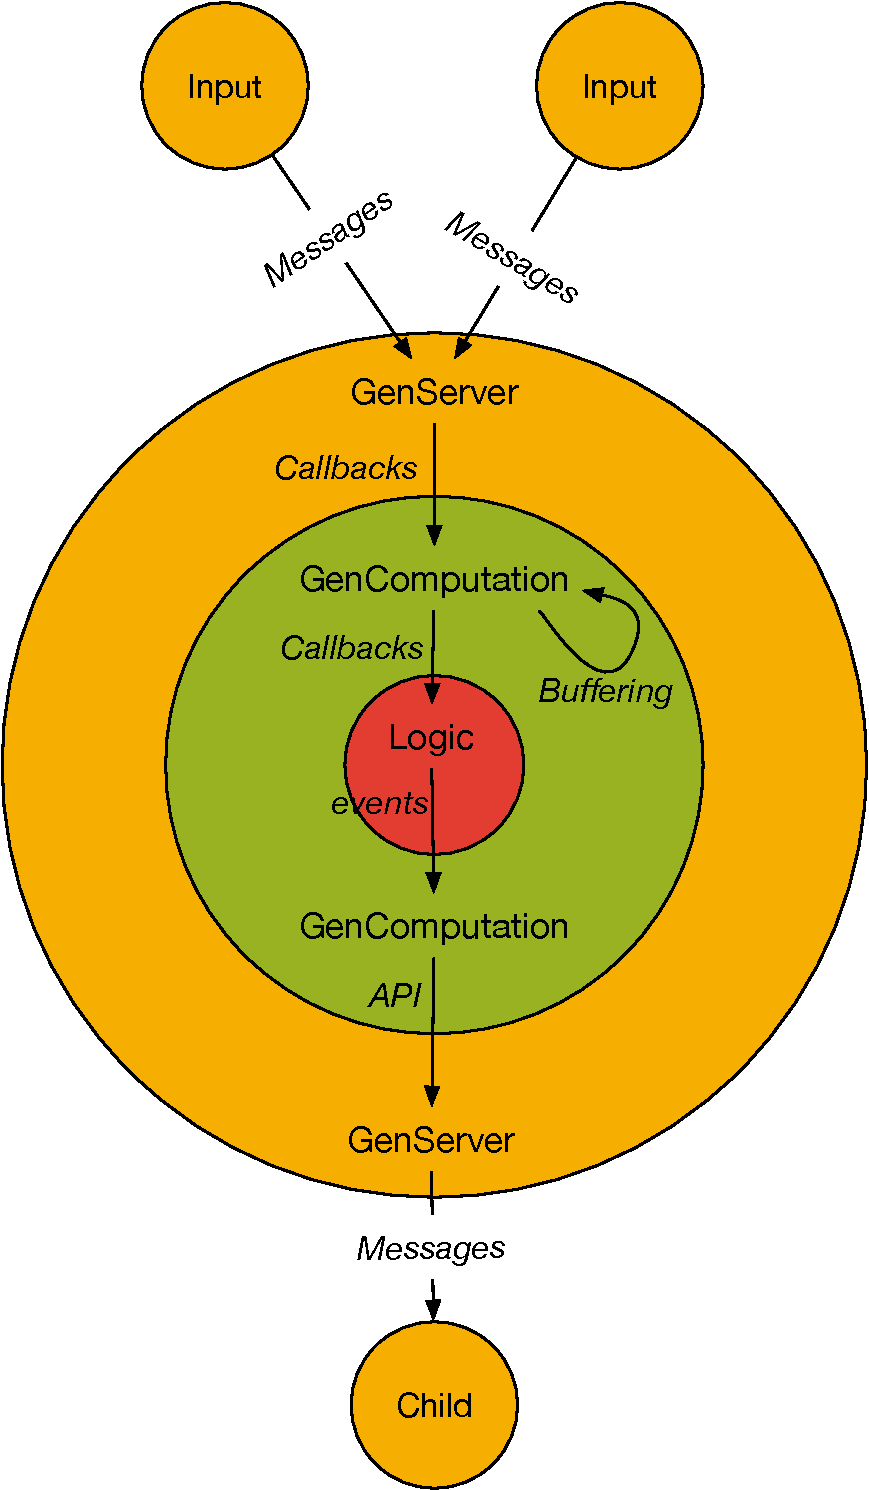
\includegraphics[width=\textwidth,height=0.9\textheight,keepaspectratio]{content/figs/node_architecture}
  \caption[Control flow of a node]{Schema of the control flow of a node. A node interacts with other nodes using the \emph{GenServer} abstraction, buffers events using the \emph{GenComputation} abstraction and performs its calculation in the \emph{logic} part. Computed events are then send to children using the same abstraction mechanisms.}
\label{fig:chap6:sec_node_impl:node_control_flow}
\end{figure}

The \emph{GenServer} abstraction is provided by the Erlang and Elixir platforms and is basically an implementation of the actor pattern mentioned above.
\emph{GenServer} provides an \gls{api} to register actors, to send messages to other actors and to handle incomming messages as well as maintaining the actor state.
Furthermore \emph{GenServer} enables monitoring, crash recovery and hot code upgrades, mechanism that are not used in TesslaServer as of now.

The next layer is provided by the \emph{GenComputation} abstraction.
Before examining its responsibilities we will look at its implementation.
\emph{GenComputation}, similar to \emph{GenServer}, heavily relies on Elixir metaprogramming, which is achieved with macros.
Elixir uses macros, a mechanism mainly known from the LISP programming language.
Macros enables the programmer to write code that generates further code.
Since all nodes perform a similar task, performing computations on one or more input streams, it makes sense to generate code for shared responsibilities instead of duplicating this kind of code for every node.
This use of macros achieves a similar goal as inheritance in object oriented programming languages, namely code reuse.

Let's now focus on the responsibilities of \emph{GenComputation}.
When a node receives a message from another node, the message will be handled by the \emph{GenServer} abstraction.
\emph{GenServer} itself requires the user to implement a callback method which is responsible for actually handling a received message by updating the state or sending new messages as required.
Since TesslaServer uses exactly one format for messages \emph{GenComputation} is able to handle them for all actual node implementations in a general way and will only invoke actual node logic when needed.
The concrete handling of messages differs beween the two versions of TesslaServer whose details are described in \Cref{sec:implementation:tesslaserver:v1,sec:implementation:tesslaserver:v2}.

On a high level \emph{GenComputation} stores messages in a buffer until it can be sure that all inputs have progressed since the last time outputs were generated by the node, which means that either new events can be generated or at least the output stream can be progressed.
A similar concept is presented in~\cite{Hall2011} which we discussed in \Cref{sec:related:stream_based:beepbeep} called the \emph{front} of the input streams.
Because BeepBeep is not using timed specifications, the computation of the front is easier: the head of each input when every input has at least one event buffered.
For \gls{tessla} the computation of the \emph{front} is not so easy, because the timestamps of the events in the front can differ.
As a result, \emph{GenComputation} has to perform multiple steps to determine the appropriate actions to take based on the events of the front.
The exact steps are described in the respective sections of the two versions of TesslaServer.
When \emph{GenComputation} has determined that at least one new transformation can happen it invokes the actual node logic by invoking a callback method that each node has to implement.

\subsection{TesslaServer V1: Stream passing}
\label{sec:implementation:tesslaserver:v1}

The first version of TesslaServer was built with two goals in mind: safety and hiding complexity.
This led to implementation decisions that had had big performance impacts (see \Cref{sec:evaluation:runtime_benchmarks}) and made it hard to implement complex node types.

One of the main ideas of this implementation is to make streams a central data structure that is able to guarantee some safety aspects like the ordering of events.
Each node maintains a number of streams: one for each parent node and one output stream.
Whenever a node computes new events, its output stream is updated and the whole updated stream is send to all of its children.
When a node receives a message from a parent node containing an updated stream, the node will update its own state by replacing the last saved stream from the parent with the newly received.
Then the node will determine if with this updated stream new events can be computed.
To do so the node looks at the input stream with the minimal progress and compare it with the progress of its own output.
If these two timestamps are equal, the node cannot produce a new front, since at least one input has not progressed since the last computation.
Only if the minimal progress of all inputs is bigger than the progress of the output the node has to perform the appropriate computations.

This is implemented by generating a sequence of partial fronts for specific timestamps as follows:

\begin{enumerate}
  \item Look at all input streams and find all events that happened after the progress of the output upto the minimal progress.
  \item Take the timestamps of these events in chronological order. We call these timestamps the \emph{change timestamps} since they denote that at least on one input stream something has changed.
  \item Iterate over the timestamps in order and build partial fronts by getting all events that happened on any input stream at that timestamp.
  \item\label{sec:implementation:tesslaserver:v1:item_logic_call} Invoke the actual logic of the node for each partial front to perform the corresponding transformation.
  \item Add the generated events to the output stream and send the updated output stream to all children.
\end{enumerate}

It is important to understand that all steps except Step \ref{sec:implementation:tesslaserver:v1:item_logic_call} are performed by the \emph{GenComputation} abstraction.
Hence, a node implementation - at least in theory - only has to implement the logic to combine a partial front to a new output.

The problems of this approach are twofold.
First, to implement more complex node types it was necessary to overwrite a lot of the provided abstractions, for example to manipulate timestamps.
But more important were scalability issues.
Since every node stores a copy of all input streams in its state and streams contained all events produced, the \gls{ram} usage grows exponentially with the number of nodes and input events used to evaluate a specification.
This can be seen in \Cref{sec:evaluation:runtime_benchmarks:num_events}.
Another problem is that the messages between nodes also grow with the number of events, since the whole stream is sent every time.

To alliviate these issues the TesslaServer v2 architecture was designed.

\subsection{TesslaServer V2: Event passing}
\label{sec:implementation:tesslaserver:v2}

The second version used the insights of the first version to provide better abstractions.
Scalability and handling complex node types were the main goals of the new architecture.

To achieve these goals some changes has to be made.
Streams are no longer an explicit data structure in the system but mere an attribute of events to denote on which stream they happened.
The new architecture of \emph{GenComputation} achieves a simpler and clearer control flow of nodes and a very small \gls{api} at the cost of some safety guarantees, which explicit streams provided.

In the new architecture simple node types implement more logic, since they have to decide how to handle progress events.
This is necessary in the new architecture to propagate that a stream has progressed to a new timestamp without an event happening on it.
In the old architecture the \emph{GenComputation} abstraction handled these cases for all nodes, which was not appropriate for some node types.
To avoid too much code duplication the new architecture provides a new abstraction \emph{GenLifted}.
\emph{GenLifted} can be used as the building block for node types that \emph{lift} a function - which normaly would run on two values - to run on two signals.
This approach avoids the problems of the old architecture by moving concerns out of the base \emph{GenComputation} abstraction and making it optional to use the new \emph{GenLifted} abstraction.

The new approach to sending messages between nodes is to send each generated event as one message.
This will lead to an overall increase in messages but simplifies the handling of each individual message.
In the new architecture, nodes contain a buffer for each parent node as part of their state.
A node saves all events received from that parent, that were not part of a front upto that point in time, in this buffer.
The process of handling new messages and computing the partial fronts implemented in the new version of \emph{GenComputation} is the following:

\begin{enumerate}
  \item Add the newly received event to the end of the buffer that stores events of that parent node.
  \item Test if on each buffer at least one event is stored.
    \begin{itemize}
      \item End if at least one buffer has no events.
    \end{itemize}
  \item Else determine the minimal timestamp over the first events of all buffers.
  \item Remove all events from the head of the buffers with that exact timestamp, as this set of events form a partial front.
  \item\label{sec:implementation:tesslaserver:v2:item_logic_call} Invoke the actual logic of the node for the partial front to perform its transformation.
  \item This will generate at least a new progress event or one or more normal events: send these events to all children of the node.
  \item Go to Step 2.
\end{enumerate}

Note again how only at Step \ref{sec:implementation:tesslaserver:v2:item_logic_call} the actual node logic is invoked, meaning only that part has to be implemented for each new node type.
Nonetheless this procedure adds more responsibilities to the programmer of new node types.
In the old approach the actual node logic did not have to handle progress events and caching of events that are important for future computations.
This can be described as the concept of making complexity explicit.
Because the implementation has to actually handle complex edge cases in contrast to the old approach which tried to hide this complexity.

One side effect of the new implementation is that one limitation on input traces is no longer needed.
In the first implementation traces had to be totally ordered over all streams, but the new implementation works as long as traces are ordered per stream.
This is especially useful when using traces that were generated by multithreaded systems.
In the systems where one can assume that each stream in the trace is exclusive for one thread the generated trace file can be directly fed to TesslaServer.
This can easily be achieved by including a unique identifier per thread in the stream identifier.

\section{Instrumentation Pass}
\label{sec:implementation:instrumentation}

While the implementation of the actual runtime was the main goal of this thesis another project was also developed, mainly to provide test traces to the runtime.
We describe the used technologies in this chapter, since the project uses some interesting technologies and can be extended to support a wide variety of trace data generation.

When no suitable test data for the runtime could be found the need for a tool to generate traces arised.
As reasoned in \Cref{sec:related:traces} all trace data that was available was not suitable for \gls{tessla} for a number of different reasons.
Therefore a tool was implemented to generate traces tailored towards evaluating \gls{tessla}.
This did open up the opportunity for the runtime as a trace collection tool.
One of the central ideas of the runtime is, that it does not make assumptions about the platform of the monitored program.
While code instrumentation with the goal to emit a trace obviously relies on the language in which the code is written, the \gls{llvm} project provides abstractions that can be used to implement an instrumentation mechanism that does not rely on the language the instrumented code was written in.

To understand how this is possible recall \Cref{sec:related:traces:llvm} and the way \gls{llvm} works.
A frontend compiles code from a source language into an \gls{ir}, performs compiler passes on the \gls{ir} and then finally compiles into native machine code.
If the instrumentation pass works at the level of the \gls{ir} it would work for all languages that have a frontend for \gls{llvm}.

It is easy to implement such an instrumentation with the provided \CC \gls{api} from \gls{llvm} to implement compiler passes that can analyse and transform \gls{ir} code.
The implementation uses the \emph{ModulePass}\footnote{\url{http://llvm.org/docs/doxygen/html/classllvm_1_1ModulePass.html}} base class to analyse whole modules.
Modules represent constructs like classes from C and \CC in \gls{ir}.
A module consists of \emph{Functions}\footnote{\url{http://llvm.org/docs/doxygen/html/classllvm_1_1Function.html}}.
On invocation implemented \emph{ModulePass} iterates over the \emph{functions} and checks if the current function is one that should be instrumented.
If so it builds a \emph{CallInst}\footnote{\url{http://llvm.org/docs/doxygen/html/classllvm_1_1CallInst.html}}, which is the \gls{ir} equivalent of calling a function.
The \emph{CallInst} will call a specified log method provided by a logging library.
The instruction is then inserted as the first instruction of the \emph{Function} that is instrumented.

At runtime the instrumented program will then log an event everytime the instrumented function is called.
Events generated by the instrumented program will have the format shown in \Cref{listing:instrumentation_trace_data}.

\begin{lstlisting}[numbers=none,float,caption={[Trace data format of the instrumentation pass]Trace data generated by the instrumentation pass. Each line represents an event and each event consists of four pieces seperated by spaces: a stream name, an optional value and the timestamp in unix format followed by the amount of microseconds since that timestamp.},label=listing:instrumentation_trace_data]
variable_values:write_ptr 843071489 1463991050 176761
variable_values:write_ptr 843071490 1463991050 176832
function_calls:process nil 1463991050 176901
\end{lstlisting}

Out implementation of the compiler pass works and was used to generate authentic test data, but it is limited and has some remaining challenges.
As we will see in \Cref{sec:evaluation:instrumentation_benchmarks} the pass can add a lot of overhead and interfere with compiler optimizations.
As a first measure to reduce the overhead the logging mechanism is implemented on top of a library called \emph{zlog}\footnote{\url{https://github.com/HardySimpson/zlog}} to buffer generated events.
Without this buffer the overhead would be much higher since constant writes of the generated events to an output device would have to happen.

A second measure is that the pass will only instrument functions that are specified by the user when invoking the pass.
This enables the generation of multiple different instrumented versions of the same code, of which each will only generate traces that are interesting for a certain specification.
For example one could have two instrumented versions of the same code, one which generates events used by a specification to monitor buffer size limits and another which generates events used by a specification describing performance constraints.

As of now the instrumentation will also produce erroneous traces when the instrumented program is multithreaded and will generate events on more than one stream.
Due to race conditions the logged events can then be in the wrong order with respect to their timestamps.
For offline monitoring this can be solved by simply reordering the events, but for online monitoring this is not possible.
For the second version of TesslaServer the problem only occurs when different threads can generate events with the same stream, since this version only requires the inputs to be totally ordered over the same input stream.
This can be solved by adding a thread unique identifier to the stream name and adapting the specifications to take into account that events might happen on different threads out of order.

As a final limitation the current instrumentation pass only supports function calls to be instrumented.
To do so it would have been enough to implement a \emph{FunctionPass}\footnote{\url{http://llvm.org/docs/doxygen/html/classllvm_1_1FunctionPass.html}}.
A \emph{ModulePass} was chosen because the pass could be easily expanded to generate other events as well, for example function returns, variable definitions, variable overwrites and assignments of null values.


% !TEX root = ../thesis.tex
%
\chapter{Evaluation}
\label{sec:evaluation}

In this chapter performance characteristics of the implemented runtime and also of the instrumentation pass are presented.
To do so both systems are tested under a number of different circumstances to get an overview of how they might perform in real world usage.
As the complete benchmark data is to big in this chapter only summarys are presented.
The complete datasets can be found in \Cref{sec:appendix}.

\section{Runtime Benchmarks}
\label{sec:evaluation:runtime_benchmarks}

Over the course of this thesis two different approaches to handling the progress of streams in the runtime are explored, which were also briefly mentioned in \Cref{sec:definitions:run}: progress timestamps and progress events.
Progress timestamps were used first, which worked, but lead to big overhead when a great number of computations had to happen, since the whole stream had to be send to all children of the node that performed the computation.
Therefore, later the runtime was refactored to use progress events, so that only events had to be sent between nodes.
The following benchmarks will show the performance characteristics of both approaches under different circumstances.

\subsection{Number of Processors}
\label{sec:evaluation:runtime_benchmarks:num_cores}

Since one of the main motivations to choose Erlang as the platform for the runtime was its support for parallel execution on many processor cores, we explore the performance characteristic in regard to available cores in this section.
To do so a simple \gls{tessla} specification is given, that includes as many nodes as the maximal number of processors available.
Such a spec for eigth processors is given in \Cref{listing:runtime_parallel_spec_8}.

\begin{figure}
  \lstinputlisting[caption=\gls{tessla} specification with eight nodes on the critical path,label=listing:runtime_parallel_spec_8]{content/code/parallel_8.spec}
\end{figure}

The specification is evaluated over appropriate traces with a specified amount of processor cores available.
The needed time of the evaluation engine from its start until it emits the conclusion, that the stream \(\mathit{done}\) is \(\mathit{true}\), is measured for different amounts of processors.
All benchmarks were performed on the same machine  with upto 16 cores and 48GB of RAM.
\Cref{fig:chap_eval:runtime_num_cores} shows the results of the benchmarks.
The complete data can be found in \Cref{table:tessla_server_v1_num_cores_data,table:tessla_server_v1_num_cores_data,table:tessla_server_v1_num_cores_data}.

\begin{figure}
  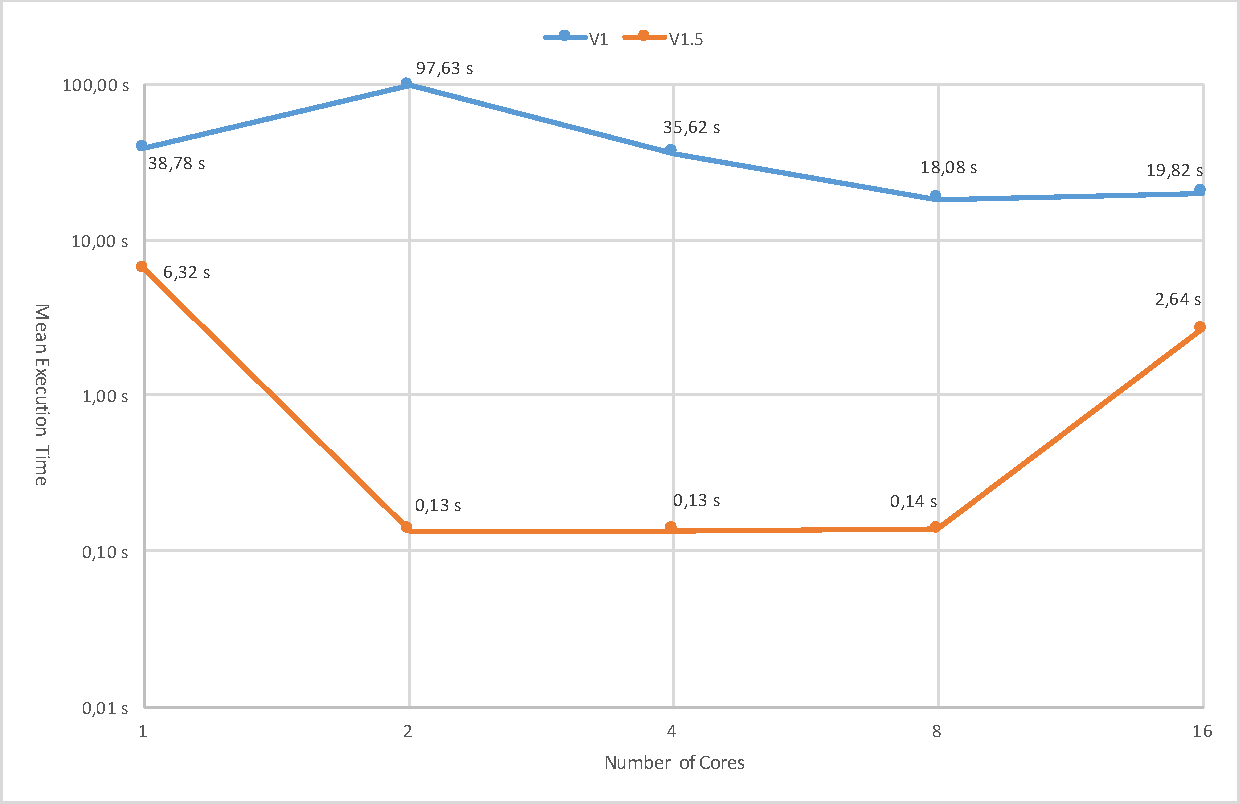
\includegraphics[width=\textwidth]{gfx/runtime_num_cores_benchmark}
  \caption[Performance of the runtime with different number of used cores]{Performance of the runtime with different number of used cores. V1 denotes the old implementation, V1.5 the adaption with limited amount of saved events and V2 the new approach.}
\label{fig:chap_eval:runtime_num_cores}
\end{figure}

One thing that was recognized during benchmarking was that the older implementation approach used big amounts of \gls{ram} and the usage grows exponentially with the amount of cores used .
For example, with two used cores the runtime would use around 2GB RAM, with 4 Cores already over 8GB.
This can be explained easily: in the old implementation all data has to be sent between all cores while in the new implementation only the generated events have to be sent around.
The excessive usage of \gls{ram} even lead to timeout under some circumstances and crashes the whole runtime.
The amount of data send between processes can even lead to negative performance impacts when more cores are added.

This behaviour was one of the main reasons to switch to a new approach.
To test if reduced \gls{ram} usage would lead to better performance and eliminate crashes, the old architecture was changed in a small way: Each stream was limited to only hold the last 20 events, all older events were thrown away.
Since the specification used for benchmarking only works on the most recent event of each stream, this would not alter the conclusion of the engine.
For example a specification computing the average of the last 21 events would not work with this adaption.
See \Cref{sec:evaluation:runtime_benchmarks:num_events} for a benchmark of \gls{ram} usage.
The obvious reduction of \gls{ram} usage of the adapted first approach motivated the decision to refactor the runtime to use the new approach.

\Cref{fig:chap_eval:runtime_num_cores} shows how the adapted first approach and second approach are both performing much better than the original one.
The graph of the adapted first version shows, that it suffers from a too high number of cores.
It is suspected that this comes from the fact that the messages between the processes are still quite big.
The new version does not only has the best performance with a single core, it also scales with more cores and does not suffer under a high number of cores.
While not tested we expect the new approach to scale very well with even more cores, especially for more complex specifications and more input events.

\subsection{Number of Events}
\label{sec:evaluation:runtime_benchmarks:num_events}

Another metric looked at, is how the runtime behaves in regard to the number of events that are fed to the engine, and therefore how many events are generated during its execution.
To obtain these metrics the specification from \Cref{listing:runtime_parallel_spec_8} is evaluated with different values for the comparision node are run.
The specification is extended to use 16 nodes, which means that each input event will generate 16 internal events.
All benchmarks in this section were performed on a processor with 4 cores at 2.4GHz speed and 8GB of RAM.

The first benchmark compares the execution time of the implementation approaches when fed with different number of input events.
\Cref{fig:chap_eval:runtime_num_events} gives an overview of the data, the whole dataset can be found in \Cref{table:tessla_server_v1_events_num_events_data,table:tessla_server_v1_5_events_num_events_data,table:tessla_server_v2_events_num_events_data}.

\begin{figure}
  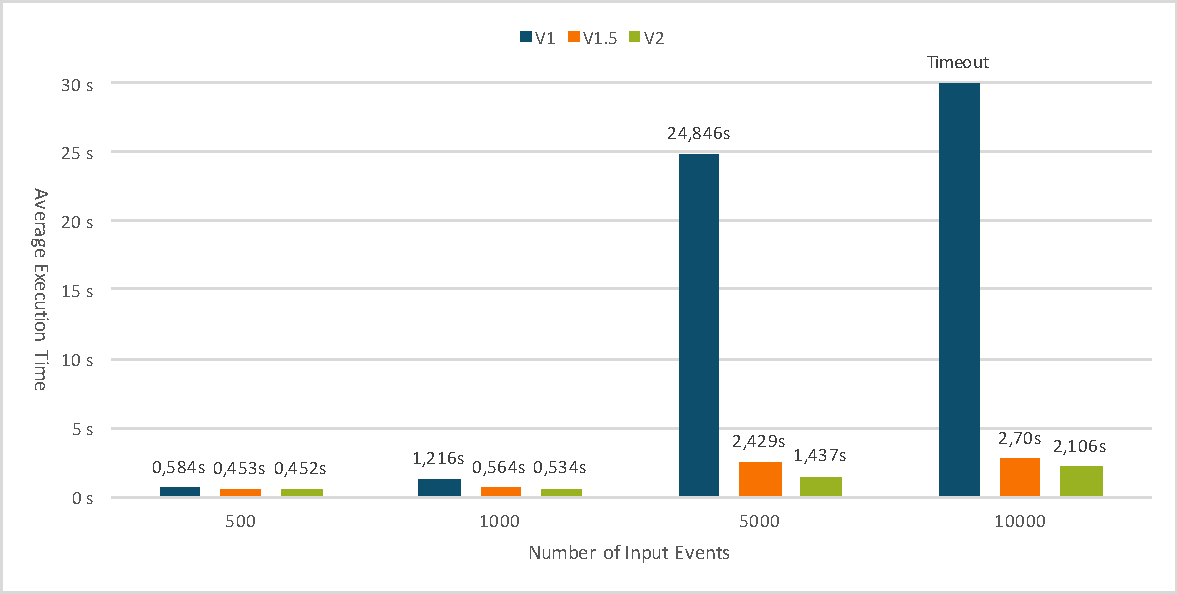
\includegraphics[width=\textwidth]{gfx/runtime_num_events_benchmark}
  \caption[Average execution time of the different implementations when fed with different amounts of input events.]{Average execution time of the different implementations when fed with different amounts of input events. V1 refers to the old approach, V1.5 to the adapted old approach and V2 to the new approach. V1 has no data for 10\,000 events since the enormous \gls{ram} usage constantly lead to timeouts.}
\label{fig:chap_eval:runtime_num_events}
\end{figure}

The numbers clearly show that the first version has big scaling problems when the number of input events grows.
The adapted approach shows, that the reduction of size of the messages is an important factor to improve the scalability.
Version 2 does perform even better than the adapted approach and also scales very well with big numbers of events.

The number of events also increase memory usage, espacially in the first implementation approach.
The second benchmark therefore tests the \gls{ram} usage of the different approaches under different number of input events.
\Cref{fig:chap_eval:runtime_ram_usage} illustrates the \gls{ram} usage of the different approaches.
The complete data can be found in \Cref{table:tessla_server_v1_events_ram_usage_data,table:tessla_server_v1_5_events_ram_usage_data,table:tessla_server_v2_events_ram_usage_data}.

\begin{figure}
  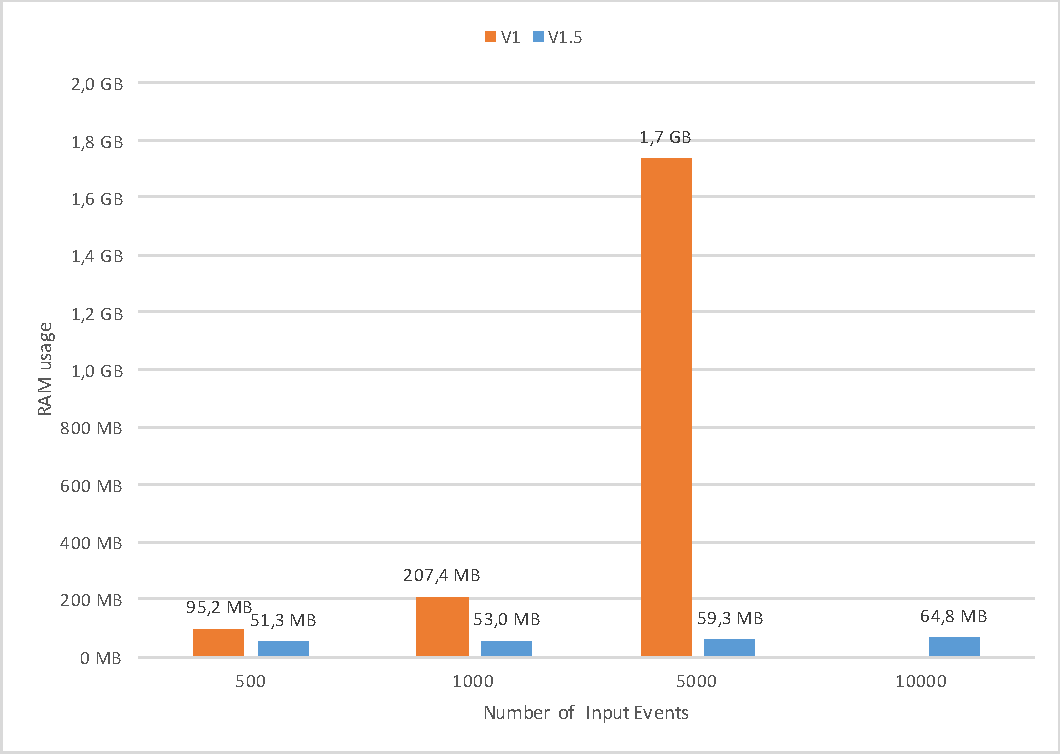
\includegraphics[width=\textwidth]{gfx/runtime_ram_usage_benchmark}
  \caption[\gls{ram} usage of the different versions of the runtime]{\gls{ram} usage of the different versions of the runtime in regard to input events. V1 refers to the old approach, V1.5 to the adapted old approach and V2 to the new approach. V1 has no data for 10\,000 events since the enormous \gls{ram} usage constantly lead to timeouts.}
\label{fig:chap_eval:runtime_ram_usage}
\end{figure}

Again it can be seen how the old version does not scale well and uses an exponential amount of memory with a growing number of events.
The adapted and the new version both require a very small memory overhead and are nearly constant in their memory consumption.
The new version uses a bit more memory, we suspect this comes from the fact that more messages have to be sent between the processes and each message carries a bit of overhead.

\subsection{Number of Nodes}

As a last metric the performance of the runtime is evaluated over specifications with different amount of nodes.
Therefore the specification from \Cref{listing:runtime_parallel_spec_8} was modified to include higher number of nodes by appending more nodes computing the absolute.
All benchmarks in this section were performed on a processor with 4 cores at 2.4GHz speed and 8GB of \gls{ram}.
\Cref{fig:chap_eval:runtime_num_nodes} visualizes the performance, the complete data can be found in \Cref{table:tessla_server_v1_num_nodes,table:tessla_server_v1_5_num_nodes,table:tessla_server_v2_num_nodes}.

\begin{figure}
  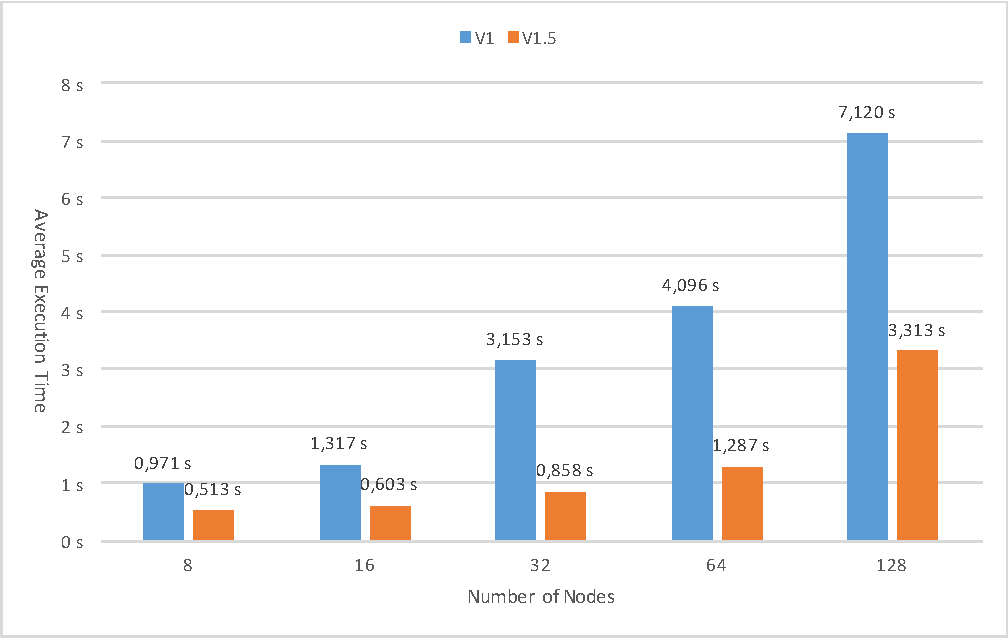
\includegraphics[width=\textwidth]{gfx/runtime_num_nodes_benchmark}
  \caption[Average execution time of the runtime over specifications with different amount of nodes.]{Average execution time of the runtime over specifications with different amount of nodes. All specifications did count the number of function calls and stopped when it reached 1\,000. V1 refers to the old approach, V1.5 to the adapted old approach and V2 to the new approach.}
\label{fig:chap_eval:runtime_num_nodes}
\end{figure}

While there is no real world data of the size of typical \gls{tessla} specifications, 128 nodes seems to be a rational upper bound.
As the data shows that all version of the runtime scale nicely with complex specification, the data even suggests a somewhat logarithmic increase of the execution time in regard to node count.
It cna also be seen that each version of the runtime has better performance than the previous one.

\clearpage

\section{Instrumentation Benchmarks}
\label{sec:evaluation:instrumentation_benchmarks}

After the evaluation of the runtime itself it remains to evaluate the C instrumentation program.
Note that the instrumentation is mostly a proof of concept and its main purpose for now was to generate test data for the runtime.
But it seems feasible that it can be optimized and extended to become a general purpose trace collection tool, therefore some benchmarks were performed.

For reliable trace collection of software the performance impact of the instrumentation is important.
To measure this a trivial C program was exercised with and without instrumentation.
The program increments each integer from 0 to 100\,000\,000 by one and, if the incremented number is divisible by a given parameter \(c\), adds it to an intermediate result.
Note that the program  can and will perform some integer overflows.
The code is shown in \Cref{listing:instrument_benchmark_code}.

The code is then instrumented to log each call of the \lstinline{add} method.
For each benchmark the compiled program was run 50 times.
All benchmarks in this section were performed on an Intel Core i5 with four cores at a clock speed of 2.4GHz and 8GB of Ram.

\begin{figure}[!hb]
\lstinputlisting[language=c, label=listing:instrument_benchmark_code, caption=Example C program for benchmark purposes]{content/code/instrument_benchmark.c}
\end{figure}


\subsection{Performance Comparison with non Instrumented Code and Compiler Optimizations}
\label{sec:evaluation:instrumentation_benchmark:instr_vs_non_inst}

One interesting metric is the intrusiveness of the instrumentation, describing how an instrumented program performs in contrast to the same program without the added instrumentation.
For this the parameter \(c\) of the example program is set to 100, so that around 1\% of all function calls are instrumented.

One thing that can be recognized is that the impact of instrumentation is not predictable when using compiler optimizations.
Aggressive compiler optimizations can remove function calls or inline values if the optimization does not change the program behaviour.
When instrumentation calls are added no such optimization can happen, since otherwise the behaviour of the program would be altered, namely the logging would be removed when the function calls are removed.

Therefore we compare the instrumented and non-instrumented code for all optimization levels.
The comparison can be seen in \Cref{fig:chap_eval:instrument_benchmark_results}.
The complete data can be found in \Cref{table:non_instrumented_optimizations_benchmark,table:instrumented_optimizations_benchmark}.

\begin{figure}
  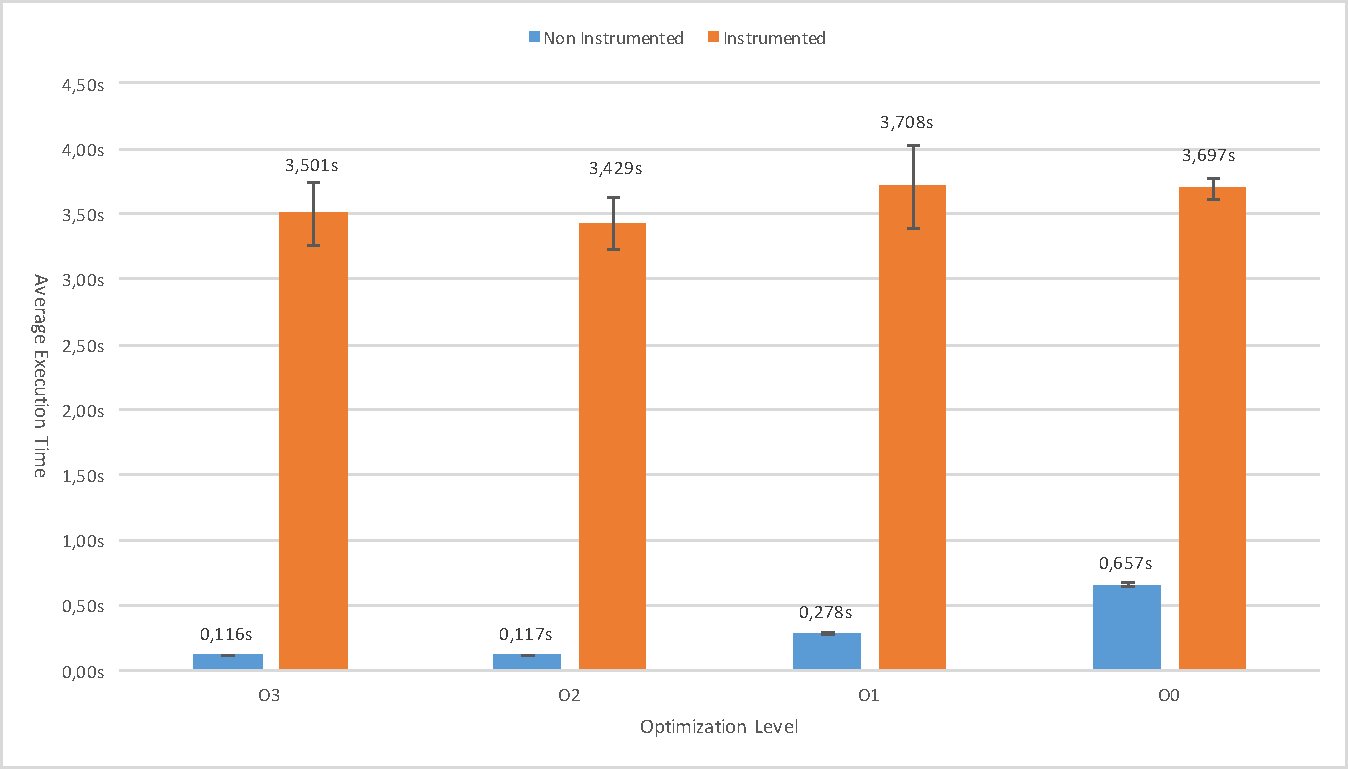
\includegraphics[width=\textwidth]{gfx/instrumentation_time_benchmark}
  \caption{Performance Comparision of an example C program with and without instrumentation.}
\label{fig:chap_eval:instrument_benchmark_results}
\end{figure}

The choice to instrument around 1\% of the function calls was made arbitrary after some experimentation showed that a higher amount leads to huge performance impacts as shown in \Cref{sec:evaluation:instrumentation_benchmark:instr_amount}.
Intuitively it sounds reasonable that in a real life example only a small subset of the function calls are interesting for trace generation, since \gls{tessla} specifications should be used to monitor only critical parts of a system.

\subsection{Performance Impact in Regard to Instrumentation Percentage}
\label{sec:evaluation:instrumentation_benchmark:instr_amount}

To further investigate the impact of instrumentation we will look at the performance impact with respect to the percentage of function calls that are instrumented.
Therefore the variable \(c\) of the program is changed, which leads to different amount of calls to the instrumented function.
For all values the program was compiled with the maximal optimization setting.
In \Cref{fig:chap_eval:instrument_benchmark_amount_results} the results of changing the parameter can be seen.
The complete dataset can be found in \Cref{table:instrumented_amount_benchmark}.

\begin{figure}
  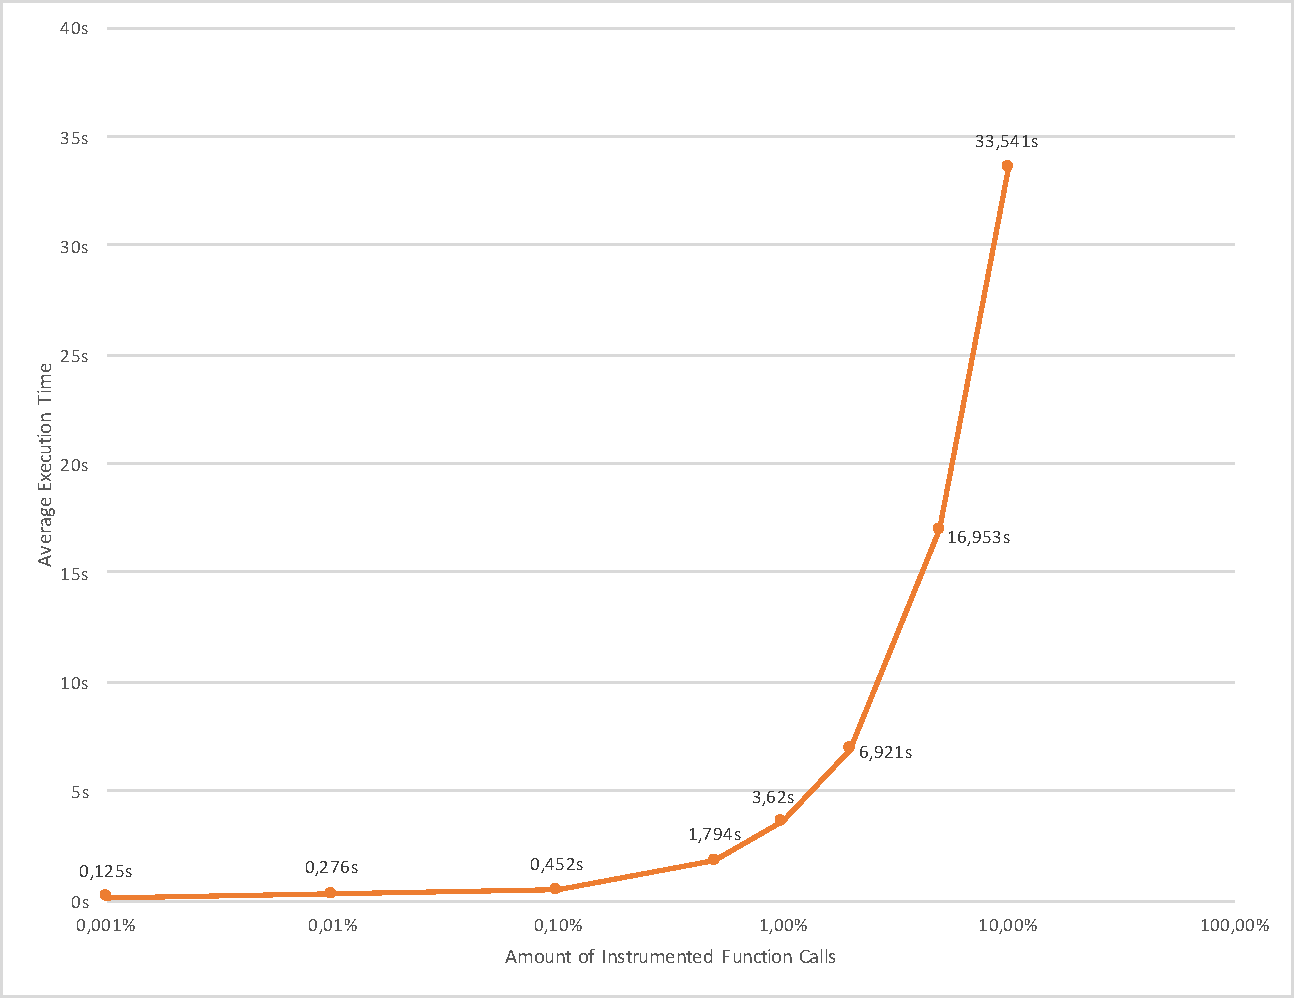
\includegraphics[width=\textwidth]{gfx/instrumentation_amount_benchmark}
  \caption{Execution time of a program with different amount of calls to an instrumented function}
\label{fig:chap_eval:instrument_benchmark_amount_results}
\end{figure}

Note that the \(x\)-axis is logarithmic.
As expected the performance impact scales directly with the amount of calls to the instrumented function.
At some point no more speed up will happen, since no calls to the instrumented functions will be made.

\section{Practical Examples}
\label{sec:evaluation:runtime_examples}

Additionally to the theoretic benchmarks it was also important to evaluate the runtime against some more practical examples and test a bigger amount of node types.
While the specifications for the benchmarks from the previous section did use some node types and showed that these types perform the correct computations (else the benchmarks would not have worked), they only used a subset of all available types.
Thus the following examples concentrate on a wider range of different nodes.

To do so traces from real world examples were collected, either with the developed instrumentation pass or by adjusting existing logs to fit the needs of \gls{tessla}.
The programs or traces were then modified to deliberately include errors to test if appropriate \gls{tessla} specifications will find them when evaluated in the runtime.

% \subsection{Ringbuffer Examples}

As the main source for test trace data a ringbuffer, implemented in C, was modified by the instrumentation to log specific events.
The code of the ringbuffer can be found in \Cref{listing:ringbuffer}.
Events that are logged are of two types: calls to the \lstinline{process} function and changes of the \lstinline{write_ptr} variable.
The generated traces can be used for a variety of specifications, inlcuding performance tests, race conditions or wrong initilizations.

The Following specifications were tested over the traces:

\begin{itemize}
  \item Data is only processed when it is available, meaning that at each point of the trace the amount of changes of \lstinline{write_ptr} is bigger than the number of calls to \lstinline{process}.
  \item The given buffer size of five is never exceeded, meaning the difference of the amount of changes of both event types is never bigger than five.
  \item Everytime new data is added, there is a call to process within the next milisecond.
\end{itemize}

The specifications were intentionally chosen and written in such a way, that they use a big amount of different nodes.
The actual \gls{tessla} specifications used to describe the requirements can be found in \Cref{sec:appendix:tessla_specs}.
For each of these specification the traces were deliberately altered to violate them.
Evaluation of the specifications over the traces with TesslaServer always led to the correct conclusions.

% !TEX root = ../thesis.tex
%
\chapter{Conclusion}
\label{sec:conclusion}

In this chapter we will revisit the work done in the whole thesis and see which parts remain to be done.
In the final section an overview of future work is given, highlighting challenges that can be approached based on the work that is already done.

\section{TesslaServer}

As the evaluation in \Cref{sec:evaluation:runtime_benchmarks,sec:evaluation:runtime_examples} shows the implemented runtime is able to evaluate a variety of specifications in a performant way.
The new architecture for the runtime improved the performance in many ways, especially enabling the evaluation of complex specifications with many input events.
Nonetheless it has to be noted that the runtime at the moment is mainly a proof of concept and isn't tested under real life circumstances or with actual systems.

At the moment there are two drawbacks of the runtime that are based on limitations of the current version of the \gls{tessla} compiler.
The limitations are missing type information and missing output information.

Let's first understand the lack of type information and the impact of the runtime.
The \gls{tessla} compiler is able to infer a lot of type information, therefore making it possible to omit type information from \gls{tessla} specifications.
Many functions in \gls{tessla} are generic over the type they consume or produce.
Recall that each function in \gls{tessla} is generic, since they work either on signals or eventstreams which carry a type themself, so a function could have the output type \lstinline{Events<Int>} or \lstinline{Signal<Boolean>}.
Furthermore a function can be generic not only over the type of the values of its streams but also what kind of stream (signal or eventstream) it consumes or produces.
Also the same function can be defined over different aritys, for example an \emph{add} function could be defined for 2, 3 or any number of arguments (note that \gls{tessla} doesn't support methods with a varying number of arguments, in some languages known as \emph{varargs}, as of now).

This leads to a situation where for example the \emph{delay} function, which delays stream by an amount, has actually three generic types: \lstinline{Events<A>,time -> Events<A>}, \lstinline{Signal<A>,time,A -> Events<a>} and \lstinline{Events<A>, Int -> Events<A>}.
The first and second functions are delaying a stream by a certain time, the second one having a default value as the third argument, and the las function delaying the events on an eventstream by a given amount of steps, meaning the first event will be delayed to the timestamp of the second event.

The compiler is now able to match the signatures of a used function to the correct one and will check if the whole specification is correct with respect to the type system.
The problem is in the output of the compiler which doesn't contain type informations anyomore, meaning that the representation of the first and third \emph{delay} functions are exactly the same and the runtime would have to figure out which type of the function it should actually use.
For the moment two workarounds are present in the runtime and compiler until the type informations are included in the output.

The first workaround is for functions which work with signals and eventstreams and have the same arity.
To make them work without type information they are split into multiple functions, one for each argument that can take either a signal or an eventstream.
For example the two \emph{delay} functions with the same arity are split into a \emph{delayEventsByTime} and a \emph{delayEventsByCount} function.
This moves some responsibility to the user writing a spec since he has to use the right function and can't rely on the compiler to figure out the correct one.
Furthermore this leads to an increased implementation effort for the runtime, since more node types have to implemented.
The second workaround is much simpler: functions which work on streams with generic type of values (e.g. \lstinline{Signal<A>}) will use \emph{Int} as the default type and doesn't support any other types.

The desired solution to the problem is, that the compiler will somehow include the type signature of functions in the output.
The signature could than be used at runtime to dynamically convert the values of events to the matching types.

The lack of output information is easier to understand and solve.
In \gls{tessla} specifications one denotes that a stream is an output stream with the \lstinline{out} keyword.
At the moment the compiler isn't handling this keyword at all and therefore it is missing in the output.
The workaround for now is, that output nodes have to be specified when the runtime is started, therefore a typical invocation of TesslaServer looks like \lstinline[language=bash]{./tessla_server example.spec -o 4:error} where the \emph{o} flag denotes an output, 4 is the id of the node that generates the output stream and \emph{error} is a name that can be chosen by the user.

A last missing functionality we want to highlight is based on the asynchronous nature of the runtime.
Since nodes are independent of each other and share no knowledge, except the one that is explicitly shared by messages, there is no global state that can be used to track if all nodes have finished their computation.
Furthermore there is no shared progres between independent nodes in the new architecture, or in other words each source will be progressed to a different timestamp.

This leads to a problem when the trace actually ends: Think of a specification with two independent sources and a trace which contains events on the stream of the first source upto timestamp \(t_2\) but for the stream of the second stream only to the timestamp \(t_1\) with \(t_1 < t_2\).
When the trace ends the second source will have only progressed to \(t_1\) while the trace implicitly contains the information that there is no event happening on its input stream at any time later than \(t_1\).
This information could lead to new generated events of a child node, for example a \emph{timeout} node which could then lead to new output events.

A simple workaround would be to implement a \emph{flush} mechanism, which will send each source node a message that there will be no more input events and therefore they can progress to the maximal timestamp.
With this mechanism all children of sources will then receive the information that their inputs have progressed without generating new events, enabling them to also progress to the maximal time.
The information that all inputs have finished will transitively flow thourgh the whole system and at one point all nodes will have performed their final computation and the system will have generated all possible outputs.

\section{Instrumentation Pass}

In the benchmarks of the instrumentation it is obvious that it adds a lot of overhead, especially when compiler optimizations are turned on or the percentage of instrumented function calls is large.
While the overhead is big, it is stable (see the standard deviation in \Cref{sec:evaluation:instrumentation_benchmark:instr_vs_non_inst}).

For now the instrumentation should be seen as a proof of concept and test tool.
The generated traces should be mostly used to analyse test settings where compiler optimizations are turned off.
When used for timing specifications, the instrumented code can be benchmarked against a non instrumented version of the code and the results can be used to transform the actual timing requirements to corresponding ones for the instrumented code.
This will at least give an approximation of the actual results.
Also it is recommended to write small and specific \gls{tessla} specifications, so that the instrumentations only have to be applied to a small subset of functions.
Obviously it is strongly discouraged to use the instrumented code in any production setting.

Two enhancements could be easliy integrated into the instrumentation pass:
Enabling the logging of more event types, like variable reads or memory allocation, while also including data in the events and introducing a better configuration format to specify what events should be logged.

As explained in \Cref{sec:implementation:instrumentation} the compiler pass is instrumented as a \emph{ModulePass}, enabling the logging of all kinds of events.
While the logging of function calls was sufficient for testing and evaluation purposes this restriction together with the total lack of logging data is an obvious problem for more serious use cases.
The trace format already includes a field for data values and the instrumentation pass has the ability to extract data, for example function arguments or return values, from the source code it is transforming.

Also the expansion to more event types shouldn't be too complicated when harnessing the \emph{InstVisitor}\footnote{\url{http://llvm.org/docs/doxygen/html/classllvm_1_1InstVisitor.html}} mechanism.
An \emph{InstVisitor} can be used to abstract the actual iteration over the building blocks of the \gls{ir} of a program, so that the user only has to specify the transformation that should be happening when a specific instruction type is seen.
For example the instrumentation of return statements could use the \emph{visitReturnInst} \gls{api} to handle all return statements and change them to log an event.

In the context of adding more event types to the instrumentation pass the configuration format becomes a problem.
For now a user specifys each function that should be instrumented when calling the pass with an option to the compiler pass like \lstinline{-instrument FUNCTIONNAME}.
This approach obviously doesn't scale when multiple event types are implemented.
Therefore a common configuration format should be specified and the instrumentation pass should read it from a given file.
This approach would also enable the sharing of configuration files between different developers and the versioning of them using version control systems.

\section{Further Work}
\label{sec:conclusion:further_work}

In addition to the adjustments that are stated in the two previous sections there are also some ideas to extend the works from this thesis in ways that require more theoretic work and larger changes of the architecture.
This section will give an overview of these ideas and will present sketches of approaches to implement them.

\subsection{Implementation for the \glsentryname{jvm}}
\label{sec:conclusion:further_work:jvm}

While the Erlang platform is tested in production for many years and provides great performance for our implementation, the desire to provide an implementation on top of the \gls{jvm} was expressed.
The main reason for this is that the \gls{tessla} compiler itself is implemented in Scala and therefore on top of the \gls{jvm}.
An implementation using the same platform would enable the distribution of a single executable that can be used to compile and evaluate \gls{tessla} specifications all in one.
Also a runtime on the \gls{jvm} could better with monitored programs that are written in a \gls{jvm} language and therefore eliminating the need for an instrumentation pass.

The Akka project\footnote{\url{http://akka.io}} provides a Scala implementation of the actor model.
Since the runtime relies heavily on this model, Akka might enable to port it to scala in a very straightforward way.
As a side node there is also an implementation of Akka on top of the .NET platform\footnote{\url{http://getakka.net}} which might be used to port the runtime to yet another platform.

\subsection{Composition of Evaluation Engines}
\label{sec:conclusion:further_work:composition}

Another idea that is motivated from the \gls{cep} field is the composition of multiple evaluation engines.
This is somewhat contrary to the \gls{rv} approach, since \gls{rv} is aimed to answer the question, if a run of a system satisfies a given property.
Therefore a specification in \gls{tessla} that is used for \gls{rv} purposes would have exactly one output: a boolean stream denoting if the property is satisfied after a given time.

The composition of evaluation engines would only makes sense, if the output of specifications would be streams that are interesting as the input to a new evaluation engine.
As it turns out, there are no restriction applied to output streams, neither by the \gls{tessla} specification language nor the runtime.

This means that it should be possible right now to combine multiple evaluation engines with only small adjustments to the output format of the runtime.

% Different evaluation model: Pull not push
% port to genstage: Concept of backpressure -> Nodes generating events out of nothing


\subsection{Parameterized Streams}
\label{sec:conclusion:further_work:parametrization}

A quite common model in \gls{rv} are parameterized streams, where one parameterized stream represents a dynamic number of actual streams.
A very common example to highlight why parameterization is required is the specification that a user can't have more than three failed login attempts in a row.
When the number of users is not known it is not possible to write such a specification without parameterization.
A parameterized version of the specification would generate a signal for each user holding the value of failed log in attempts in a row.

The common approach to handle parameterized specifications, called \emph{slicing}, is discussed in~\cite{Chen2009a}.
The basic idea of \emph{slicing} is to partition a stream of events, where each event holds a data value, into multiple streams with respect to that data.
In context of the example specification restricting failed log in attempts the following would happen:
An input stream \lstinline{login_attempt(int, bool)} denoting that a user with the id that is the first value of the stream tried to login, where the second value denotes if the login was succesful, would be partitioned, or \emph{sliced}, by the first argument, generating a variable number of streams \lstinline{login_attempt_id(bool)}.
Each of this streams could then be evaluated by the \gls{tessla} runtime.

While streams in \gls{tessla} are already carrying data only a restricted form of generating new streams based on this data is possible.
This limited slicing can be performed for example using the \emph{ifThen} function, which can be used to get only that events of a stream that cary a specified value.
But since the real expressiveness of parameterization is based on the dynamic nature of the input data that approach is not sufficient.
Therefore, to allow parameterized streams, the \gls{tessla} specification language would have to be extended.
How exactly this extension would look like remains to be specified.

The changes required to allow slicing in the runtime shouldn't be very complex.
Basically a \emph{slice} node would have to be implemented, that has one input stream and a variable number of output streams.
Whenever the node receives an event which carries a value that wasn't seen before the node would have to start new child nodes that are responsible to handle the new stream.
Since nodes are already generated at runtime, when the evaluation engine is synthesized, it should be no problem to start new ones during the evaluation process.


% online monitoring -> possible infinite traces, important that on each stream new event finally happen.

\subsection{Easier Definition of New Node Types}
\label{sec:conclusion:further_work:node_definition}

A problem that is still present in the current architecture is how complex it is to implement new node types.
First of all the \gls{tessla} compiler needs to be changed to include the signature of the new function and to support the mapping of the function to its \gls{json} representation.
Then a corresponding node has to be implemented for the runtime.
While the \emph{GenLifted} abstraction provides a starting point for a generic generation of new node types it still requires manual work to implement new node types.

To improve this \gls{tessla} could be extended with a mechanism to somehow specify new functions without the requirement to explicitly implement them in the compiler and the runtime.
A somehow related technique that is already present in \gls{tessla} are macros which can be used in a specification to compose existing functions into a new one.
While this enables the user to write more expressive specifications by leveraging reuse of common subexpressions in a specification it doesn't support the generation of new functions.

One approach that looks promising is presented in~\cite{Hall2011} in the contetxt of the BeepBeep tool.
In BeepBeep computations can be generated by combining two base parts, \emph{processors} and \emph{functions}.
A processor is responsible to apply a transformation on one or more streams while functions specify how the exact transformation looks like.
As an example lets look at two processors that could be implemented and how they could be combined with one function to perform different transformations.

Let the example processors be called \emph{Combiner} and \emph{Aggregator}.
The \emph{Combiner} processor is responsible for combining two input streams by applying a function for each front and the \emph{Aggregator} computes an aggregation over one stream by applying a function to each new event combined with the last computed value.
Each function that takes two input values and generates one output can be combined with these processors.
The \(+\) function when combined with a \emph{Combiner} would add the values of two streams at each position while it would compute the sum of the values of all events on one stream when combined with an \emph{Aggregator}.

As part of \gls{tessla} this approach could lead to a much smaller implementation effort for the runtime.
How exactly it could be integrated into \gls{tessla} remains to be discussed.

\subsection{Runtime Optimizations}
\label{sec:conclusion:further_work:runtime_optimizations}

Optimizations: Bundle up events, throw away unneeded progress events in  bundles
  For some notes only subset of inputs is important for output progress (think if then else)
    -> Some things may be optimized by compiler (literal as cond to ite) others only during evaluation.


\subsection{Error prevention}
\label{sec:conclusion:further_work:error_prevention}
Ways of sending observations back to the program to recover from or prevent errors


\subsection{Instrumentation Pass}
More fine grained instrumentation pass config: restrictions etc
TODO: Timing model, maybe somehow harness Vector clocks -> would  compplicate instrumentation! Also would need support in TeSSLa language.
Configuration file for instrumetnation -> e.g. include conditions

% !TEX root = ../thesis.tex
%
\chapter{Appendix}
\label{sec:appendix}

\section{Runtime Benchmark Data}
\label{sec:appendix:runtime_benchmark_data}

This section includes all data from the benchmarks of TesslaServer.

\subsection{Execution Time in Regard to Used Processor Cores}
\label{sec:appendix:runtime_benchmark_data:execution_time_cores}

\begin{table}[!htb]
  \centering
  \caption{Execution time of multiple runs of TesslaServer V1 with 10\,000 input events with different number of used processor cores.}
  \label{table:tessla_server_v1_num_cores_data}
  \begin{tabular}{clllll}
    Run \# &\multicolumn{1}{c}{1} & \multicolumn{1}{c}{2} & \multicolumn{1}{c}{4} & \multicolumn{1}{c}{8} & \multicolumn{1}{c}{16} \\ \hline
    1 & 38.2684 s & 95.8390 s  & 33.2289 s & 18.3235 s & 21.9672 s \\
    2 & 38.9833 s & 98.9827 s  & 32.3660 s   & 17.9681 s & 19.4063 s \\
    3 & 38.1630 s & 77.4360 s  & 36.0462 s & 17.0076 s & 27.6495 s \\
    5 & 38.4424 s & 222.9723 s & 29.4773 s & 17.2925 s & 17.3606 s \\
    6 &  39.2239 s & 75.5560 s  & 32.1869 s & 15.3906 s & 19.1662 s  \\
    7 &  38.7815 s & 81.0928 s  & 44.7217 s & 18.3882 s & 21.9974 s \\
    8 &  38.7514 s & 119.1012 s & 38.0911 s & 18.0104 s & 20.2454 s \\
    9 &  37.8491 s & 60.2407 s  & 35.0671 s & 17.9517 s & 17.2825 s \\
    10 &  38.2721 s & 83.5956 s  & 37.5839 s & 17.1108 s & 15.5887 s \\
    11 &  38.5657 s & 105.2514 s & 43.8580 s & 15.8287 s & 22.0196 s \\
    12 &  38.1699 s & 75.6985 s   & 32.4470 s  & 15.7641 s & 18.3230 s \\
    13 &  37.9775 s & 104.0994 s & 37.0281 s & 24.5554 s & 17.0857 s \\
    14 &  38.8215 s & 75.0534 s    & 34.8001 s & 14.3733 s & 19.5598 s \\
    15 &  38.3913 s & 74.5584 s  & 32.7344 s & 17.9163 s  & 17.3179 s \\
    16 &  40.4536 s & 111.3214 s & 35.7434 s  & 16.6162 s & 20.2855 s \\
    17 &  39.0735 s & 87.0386 s  & 35.6367 s & 15.5962 s & 21.7681 s \\
    18 &  38.8830 s & 114.2697 s & 33.4537 s & 28.1556 s & 17.2382 s \\
    19 &  39.0799 s & 103.1956 s & 32.7134 s & 17.7034 s & 23.5276 s \\
    20 &  39.3866 s & 117.2423 s & 39.1457 s & 15.6895 s & 18.4146 s
  \end{tabular}
\end{table}

\begin{table}[!htb]
  \centering
  \caption{Execution time of multiple runs of TesslaServer V1.5 with 10\,000 input events with different number of used processor cores}
  \label{table:tessla_server_v1_5_num_cores_data}
  \begin{tabular}{clllll}
    Run \# & \multicolumn{1}{c}{1} & \multicolumn{1}{c}{2} & \multicolumn{1}{c}{4} & \multicolumn{1}{c}{8} & \multicolumn{1}{c}{16} \\ \hline
    1 &  6.3722 s & 0.1256 s & 0.1309 s   & 0.1378 s & 2.6756 s \\
    2 &  6.2417 s & 0.1300 s & 0.1333 s & 0.1444 s & 2.6292 s   \\
    3 &  6.2953 s & 0.1301 s   & 0.1325 s & 0.1379 s & 2.6453 s \\
    5 &  6.5148 s   & 0.1433 s & 0.1315 s & 0.1451 s & 2.5836 s \\
    6 &  6.6828 s & 0.1347 s & 0.1480 s & 0.1468 s & 2.6670 s   \\
    7 &  6.8090 s & 0.1386 s & 0.1294 s & 0.1414 s & 2.6671 s \\
    8 &  6.3252 s & 0.1307 s  & 0.1330 s & 0.1385 s & 2.7755 s \\
    9 &  6.0975 s & 0.1304 s & 0.1339 s & 0.1362 s & 2.6097 s \\
    10 & 6.1274 s & 0.1328 s & 0.1325 s & 0.1371 s & 2.6335 s \\
    11 & 5.7481 s & 0.1479 s & 0.1299 s & 0.1398 s & 2.6477 s \\
    12 & 6.0317 s & 0.1318 s & 0.1435 s & 0.1311 s   & 2.6343 s \\
    13 & 6.1565 s & 0.1293 s & 0.1260 s   & 0.1361 s & 2.6603 s \\
    14 & 6.3439 s & 0.1223 s & 0.1309 s & 0.1313 s & 2.5560 s \\
    15 & 6.3749 s & 0.1318 s & 0.1335 s & 0.1338 s & 2.6739 s \\
    16 & 6.3289 s & 0.1321 s & 0.1323 s & 0.1503 s & 2.5466 s   \\
    17 & 6.3894 s & 0.1253 s & 0.1323 s & 0.1397 s & 2.6240 s \\
    18 & 6.3943 s & 0.1288 s & 0.1320 s & 0.1316 s & 2.6939 s \\
    19 & 6.4089 s & 0.1319 s & 0.1347 s & 0.1302 s & 2.5940 s \\
    20 & 6.3865 s & 0.1698 s & 0.1336 s & 0.1312 s & 2.6347 s
  \end{tabular}
\end{table}

\begin{table}[!htb]
  \centering
  \caption{Execution time of multiple runs of TesslaServer V2 with 10\,000 input events with different number of used processor cores}
  \label{table:tessla_server_v2_num_cores_data}
  \begin{tabular}{clllll}
    Run \# & \multicolumn{1}{c}{1} & \multicolumn{1}{c}{2} & \multicolumn{1}{c}{4} & \multicolumn{1}{c}{8} & \multicolumn{1}{c}{16} \\ \hline
    1 &  3.620s & 1.598s & 1.024s   & 0.948s  & 1.010s \\
    2 &  3.483s & 1.650s & 0.964s & 0.974s & 0.971s \\
    3 &  3.488s & 1.753s & 0.989s & 0.959s & 0.989s \\
    5 &  3.439s & 1.597s & 1.009s   & 1.033s & 1.082s \\
    6 &  3.521s & 1.651s & 1.013s   & 0.931s & 1.151s \\
    7 &  3.448s & 1.725s & 0.976s & 0.987s & 0.982s \\
    8 &  3.550s & 1.648s & 0.994s & 0.979s & 1.098s \\
    9 &  3.496s & 1.624s & 1.098s & 0.967s & 1.137s   \\
    10 & 3.586s & 1.615s & 1.039s & 1.011s & 1.042s \\
    11 & 3.504s  & 1.634s & 1.092s & 1.075s & 1.101s \\
    12 & 3.443s & 1.580s & 0.944s & 1.003s & 1.060s \\
    13 & 3.840s & 1.609s & 1.017s & 1.009s & 1.071s \\
    14 & 3.605s & 1.579s & 0.964s & 1.083s & 1.189s \\
    15 & 3.499s & 1.535s & 0.981s & 0.997s & 1.023s  \\
    16 & 3.535s & 1.608s & 0.989s & 1.287s & 1.121s   \\
    17 & 3.446s & 1.739s & 1.015s & 1.007s & 1.129s \\
    18 & 3.505s & 1.544s & 1.047s & 1.175s & 1.161s \\
    19 & 3.586s & 1.680s & 1.013s & 1.035s & 1.067s   \\
    20 & 3.377s & 1.611s & 1.008s & 1.096s & 1.100s
  \end{tabular}
\end{table}

\clearpage

\subsection{Execution Time in Regard to Number of Input Events}
\label{sec:appendix:runtime_benchmark_data:execution_time_cores}

\begin{table}[!htb]
  \centering
  \caption{Execution time of multiple runs of TesslaServer V1 with different number of input events}
  \label{table:tessla_server_v1_events_num_events_data}
  \begin{tabular}{cllll}
    Run \# & \multicolumn{1}{c}{500} & \multicolumn{1}{c}{1000} & \multicolumn{1}{c}{5000}  & \multicolumn{1}{c}{10000} \\ \hline
    1 &  0.5815 s & 1.1913 s & 39.0046 s & timeout\\
    2 &  0.5958 s & 1.1991 s & 33.5771 s & timeout\\
    3 &  0.5963 s & 1.2122 s & 26.8252 s & timeout\\
    5 &  0.580 s  & 1.2569 s & 23.8944 s & timeout\\
    6 &  0.5948 s & 1.2280 s & 23.8837 s & timeout\\
    7 &  0.5825 s & 1.2519 s & 23.4110 s & timeout\\
    8 &  0.6271 s & 1.2636 s & 23.1929 s & timeout\\
    9 &  0.5705 s & 1.2324 s & 23.3227 s & timeout\\
    10 & 0.5765 s & 1.1783 s & 21.9043 s & timeout\\
    11 & 0.5893 s & 1.1928 s & 22.9516 s & timeout\\
    12 & 0.6101 s & 1.2759 s & 22.8377 s & timeout\\
    13 & 0.5684 s & 1.1955 s & 26.1974 s & timeout\\
    14 & 0.5746 s & 1.2047 s & 25.7536 s & timeout\\
    15 & 0.5588 s & 1.2044 s & 24.6289 s & timeout\\
    16 & 0.5698 s & 1.1958 s & 22.3709 s & timeout\\
    17 & 0.5911 s & 1.2271 s & 23.9404 s & timeout\\
    18 & 0.5955 s & 1.1981 s & 21.4453 s & timeout\\
    19 & 0.5702 s & 1.1718 s & 23.3482 s & timeout\\
    20 & 0.5863 s & 1.2571 s & 21.9753 s & timeout
  \end{tabular}
\end{table}

\begin{table}[!htb]
  \centering
  \caption{Execution time of multiple runs of TesslaServer V1.5 with different number of input events}
  \label{table:tessla_server_v1_5_events_num_events_data}
  \begin{tabular}{cllll}
    Run \# & \multicolumn{1}{c}{500} & \multicolumn{1}{c}{1000} & \multicolumn{1}{c}{5000} & \multicolumn{1}{c}{10000} \\ \hline
   1 &   0.4512 s & 0.5901 s & 2.1607 s & 2.8476 s \\
   2 &   0.4349 s & 0.5703 s & 2.0242 s & 2.8715 s \\
   3 &   0.4424 s & 0.5511 s & 2.1535 s & 2.8250 s \\
   5 &   0.4373 s & 0.5487 s & 2.1715 s & 2.7025 s \\
   6 &   0.4239 s & 0.5564 s & 2.2763 s & 2.7671 s \\
   7 &   0.4670 s & 0.5466 s & 4.2085 s & 2.6719 s \\
   8 &   0.4492 s & 0.5401 s & 2.6771 s & 2.6956 s \\
   9 &   0.4649 s & 0.6345 s & 1.9132 s & 2.5634 s \\
   10 &  0.440 s  & 0.5618 s & 1.5309 s & 2.6090 s \\
   11 &  0.4641 s & 0.5577 s & 2.5762 s & 2.6738 s \\
   12 &  0.4306 s & 0.5415 s & 1.6873 s & 2.7178 s \\
   13 &  0.4255 s & 0.5829 s & 2.0342 s & 2.7294 s \\
   14 &  0.460 s  & 0.5442 s & 3.0314 s & 2.6789 s \\
   15 &  0.4401 s & 0.5443 s & 3.2066 s & 2.6045 s \\
   16 &  0.4516 s & 0.5848 s & 2.5746 s & 2.5837 s \\
   17 &  0.4927 s & 0.5406 s & 2.4933 s & 2.7866 s \\
   18 &  0.4635 s & 0.5669 s & 2.6895 s & 2.6719 s \\
   19 &  0.4506 s & 0.5576 s & 2.2802 s & 2.7056 s \\
   20 &  0.5080 s & 0.5898 s & 2.4456 s & 2.6697 s
  \end{tabular}
\end{table}

\begin{table}[!htb]
  \centering
  \caption{Execution time of multiple runs of TesslaServer V2 with different number of input events}
  \label{table:tessla_server_v2_events_num_events_data}
  \begin{tabular}{cllll}
    Run \# & \multicolumn{1}{c}{500} & \multicolumn{1}{c}{1000} & \multicolumn{1}{c}{5000} & \multicolumn{1}{c}{10000} \\ \hline
    1 &  0.4415 s & 0.5358 s & 1.4555 s & 1.9343 s \\
    2 &  0.4569 s & 0.5471 s & 1.4538 s & 1.9907 s \\
    3 &  0.4549 s & 0.4996 s & 2.8283 s & 1.9546 s \\
    5 &  0.4569 s & 0.4985 s & 1.8618 s & 1.9731 s \\
    6 &  0.4603 s & 0.5482 s & 1.3788 s & 1.9725 s \\
    7 &  0.4610 s & 0.5489 s & 1.1817 s & 2.0493 s \\
    8 &  0.4585 s & 0.5302 s & 1.1973 s & 1.9670 s \\
    9 &  0.4407 s & 0.5581 s & 1.3172 s & 2.2681 s \\
    10 & 0.4414 s & 0.5407 s & 1.3002 s & 2.0725 s \\
    11 & 0.4392 s & 0.5349 s & 1.2226 s & 1.9567 s \\
    12 & 0.4652 s & 0.5557 s & 1.2435 s & 1.9850 s \\
    13 & 0.4436 s & 0.5462 s & 1.2375 s & 2.0038 s \\
    14 & 0.4458 s & 0.5240 s & 1.2271 s & 2.0334 s \\
    15 & 0.4480 s & 0.5093 s & 1.2287 s & 1.9577 s \\
    16 & 0.4508 s & 0.5071 s & 1.8341 s & 2.0005 s \\
    17 & 0.4498 s & 0.5390 s & 1.5943 s & 2.1850 s \\
    18 & 0.4820 s & 0.5252 s & 1.4755 s & 2.4828 s \\
    19 & 0.4365 s & 0.5576 s & 1.2696 s & 2.5152 s \\
    20 & 0.4379 s & 0.5334 s & 1.2343 s & 2.3986 s \\
  \end{tabular}
\end{table}

\clearpage

\subsection{Ram Usage with Respect to Number of Input Events}
\label{sec:appendix:runtime_benchmark_data:ram_usage_events}

\begin{table}[!htb]
  \centering
  \caption{RAM usage of multiple runs of TesslaServer V1 with different number of input events}
  \label{table:tessla_server_v1_events_ram_usage_data}
  \begin{tabular}{cllll}
    Run \# & \multicolumn{1}{c}{500} & \multicolumn{1}{c}{1000} & \multicolumn{1}{c}{5000} \\ \hline
    1 & 98.50 MB  & 182.93 MB & 1.55 GB & timeout \\
    2 & 95.47 MB  & 226.23 MB & 1.69 GB & timeout\\
    3 & 84.59 MB  & 223.75 MB & 1.62 GB & timeout\\
    5 & 102.98 MB & 185.86 MB & 1.78 GB & timeout\\
    6 & 90.24 MB  & 222.20 MB & 1.77 GB & timeout\\
    7 & 84.54 MB  & 181.79 MB & 1.75 GB & timeout\\
    8 & 89.31 MB  & 171.32 MB & 1.60 GB & timeout\\
    9 & 89.84 MB  & 228.12 MB & 1.75 GB & timeout\\
    10 & 106.07 MB & 184.48 MB & 1.67 GB & timeout\\
    11 & 89.41 MB  & 194.26 MB & 1.47 GB & timeout\\
    12 & 97.62 MB  & 163.42 MB & 1.80 GB & timeout\\
    13 & 97.54 MB  & 160.26 MB & 1.51 GB & timeout\\
    14 & 88.77 MB  & 221.16 MB & 1.96 GB & timeout\\
    15 & 99.99 MB  & 223.81 MB & 1.87 GB & timeout\\
    16 & 97.40 MB  & 216.00 MB & 1.87 GB & timeout\\
    17 & 87.62 MB  & 250.93 MB & 1.68 GB & timeout\\
    18 & 120.70 MB & 206.97 MB & 1.71 GB & timeout\\
    19 & 91.89 MB  & 246.55 MB & 1.64 GB & timeout\\
    20 & 88.91 MB  & 252.26 MB & 1.87 GB & timeout
  \end{tabular}
\end{table}

\begin{table}[!htb]
  \centering
  \caption{RAM usage of multiple runs of TesslaServer V1.5 with different number of input events}
  \label{table:tessla_server_v1_5_events_ram_usage_data}
  \begin{tabular}{cllll}
    Run \# & \multicolumn{1}{c}{500} & \multicolumn{1}{c}{1000} & \multicolumn{1}{c}{5000} & \multicolumn{1}{c}{1000}\\ \hline
    1 & 52.09 MB & 53.71 MB & 61.49 MB & 58.37 MB \\
    2 & 48.77 MB & 56.98 MB & 59.74 MB & 60.16 MB \\
    3 & 52.06 MB & 52.60 MB & 57.21 MB & 75.88 MB \\
    5 & 52.42 MB & 51.23 MB & 57.45 MB & 61.79 MB \\
    6 & 54.13 MB & 52.44 MB & 56.55 MB & 74.53 MB \\
    7 & 50.30 MB & 50.41 MB & 76.10 MB & 62.92 MB \\
    8 & 47.91 MB & 52.48 MB & 53.78 MB & 63.47 MB \\
    9 & 50.97 MB & 51.99 MB & 58.85 MB & 60.24 MB \\
    10 &52.26 MB & 51.00 MB & 57.04 MB & 59.36 MB \\
    11 &51.25 MB & 54.08 MB & 57.74 MB & 62.32 MB \\
    12 &47.60 MB & 52.06 MB & 53.92 MB & 65.00 MB \\
    13 &50.15 MB & 52.54 MB & 57.23 MB & 64.99 MB \\
    14 &51.03 MB & 52.09 MB & 59.37 MB & 64.33 MB \\
    15 &52.56 MB & 62.94 MB & 53.98 MB & 65.32 MB \\
    16 &50.79 MB & 50.54 MB & 58.80 MB & 67.25 MB \\
    17 &61.64 MB & 49.85 MB & 56.02 MB & 58.18 MB \\
    18 &50.69 MB & 51.54 MB & 60.00 MB & 59.93 MB \\
    19 &49.59 MB & 52.21 MB & 61.75 MB & 82.53 MB \\
    20 &50.04 MB & 51.91 MB & 67.09 MB & 72.43 MB
  \end{tabular}
\end{table}

\begin{table}[!htb]
  \centering
  \caption{RAM usage of multiple runs of TesslaServer V2 with different number of input events}
  \label{table:tessla_server_v2_events_ram_usage_data}
  \begin{tabular}{cllll}
    Run \# & \multicolumn{1}{c}{500} & \multicolumn{1}{c}{1000} & \multicolumn{1}{c}{5000} & \multicolumn{1}{c}{1000}\\ \hline
    1 & 50.95 MB & 51.71 MB & 65.99 MB & 71.82 MB \\
    2 & 50.55 MB & 59.71 MB & 63.25 MB & 71.65 MB \\
    3 & 52.09 MB & 50.17 MB & 73.34 MB & 79.18 MB \\
    5 & 50.45 MB & 51.35 MB & 66.12 MB & 65.73 MB \\
    6 & 62.37 MB & 52.33 MB & 75.56 MB & 72.34 MB \\
    7 & 50.24 MB & 49.91 MB & 70.64 MB & 81.99 MB \\
    8 & 49.84 MB & 51.51 MB & 61.73 MB & 70.57 MB \\
    9 & 53.22 MB & 52.20 MB & 61.24 MB & 70.05 MB \\
    10 &55.05 MB & 52.32 MB & 77.86 MB & 74.08 MB \\
    11 &51.11 MB & 50.86 MB & 65.75 MB & 66.15 MB \\
    12 &52.04 MB & 51.57 MB & 63.21 MB & 68.69 MB \\
    13 &49.97 MB & 50.91 MB & 93.26 MB & 66.23 MB \\
    14 &53.91 MB & 51.40 MB & 66.14 MB & 61.75 MB \\
    15 &49.71 MB & 68.42 MB & 71.99 MB & 67.96 MB \\
    16 &49.84 MB & 64.05 MB & 63.66 MB & 68.89 MB \\
    17 &50.39 MB & 51.54 MB & 71.29 MB & 64.43 MB \\
    18 &49.29 MB & 50.30 MB & 68.03 MB & 69.73 MB \\
    19 &52.94 MB & 61.20 MB & 64.49 MB & 67.56 MB \\
    20 &53.41 MB & 60.22 MB & 66.41 MB & 83.87 MB
  \end{tabular}
\end{table}

\clearpage

\subsection{Execution Time in Regard to Number of Nodes}
\label{sec:appendix:runtime_benchmark_data:ram_usage_events}

\begin{table}[!htb]
  \centering
  \caption{Execution time of multiple runs of TesslaServer V1 in regard to different amount of nodes in a specification}
  \label{table:tessla_server_v1_num_nodes}
  \begin{tabular}{clllll}
    Run \# & \multicolumn{1}{c}{8} & \multicolumn{1}{c}{16} & \multicolumn{1}{c}{32} & \multicolumn{1}{c}{64} & \multicolumn{1}{c}{128}\\ \hline
    1 & 0.997 s & 1.295 s & 2.893 s & 3.780 s & 7.166 s \\
    2 & 0.875 s & 1.280 s & 2.903 s & 4.139 s & 7.071 s \\
    3 & 1.269 s & 1.277 s & 2.837 s & 4.055 s & 7.083 s \\
    5 & 0.888 s & 1.262 s & 3.693 s & 3.811 s & 6.937 s \\
    6 & 0.917 s & 1.330 s & 4.930 s & 4.150 s & 7.075 s \\
    7 & 0.881 s & 1.419 s & 3.761 s & 3.826 s & 7.327 s \\
    8 & 0.959 s & 1.398 s & 3.115 s & 3.835 s & 7.158 s \\
    9 & 0.973 s & 1.294 s & 2.944 s & 4.093 s & 7.102 s \\
    10 &0.980 s & 1.257 s & 3.143 s & 4.208 s & 6.981 s \\
    11 &0.918 s & 1.285 s & 2.788 s & 4.092 s & 7.081 s \\
    12 &0.939 s & 1.329 s & 2.914 s & 4.033 s & 7.198 s \\
    13 &0.965 s & 1.225 s & 2.850 s & 3.815 s & 7.135 s \\
    14 &0.871 s & 1.320 s & 3.003 s & 3.817 s & 6.943 s \\
    15 &0.898 s & 1.336 s & 2.922 s & 3.905 s & 6.901 s \\
    16 &0.897 s & 1.357 s & 3.212 s & 3.968 s & 7.153 s \\
    17 &1.073 s & 1.401 s & 3.057 s & 4.081 s & 7.10 s  \\
    18 &1.182 s & 1.342 s & 2.759 s & 3.826 s & 7.311 s \\
    19 &1.019 s & 1.288 s & 2.945 s & 3.991 s & 7.064 s \\
    20 &0.928 s & 1.314 s & 3.304 s & 5.343 s & 7.161 s
  \end{tabular}
\end{table}

\begin{table}[!htb]
  \centering
  \caption{Execution time of multiple runs of TesslaServer V1.5 in regard to different amount of nodes in a specification}
  \label{table:tessla_server_v1_5_num_nodes}
  \begin{tabular}{clllll}
    Run \# & \multicolumn{1}{c}{8} & \multicolumn{1}{c}{16} & \multicolumn{1}{c}{32} & \multicolumn{1}{c}{64} & \multicolumn{1}{c}{128}\\ \hline
    1 & 0.474 s & 0.602 s & 0.811 s & 1.353 s & 2.134 s \\
    2 & 0.476 s & 0.605 s & 0.813 s & 1.410 s & 2.431 s \\
    3 & 0.487 s & 0.577 s & 0.884 s & 1.331 s & 2.015 s \\
    5 & 0.502 s & 0.606 s & 0.933 s & 1.273 s & 2.138 s \\
    6 & 0.511 s & 0.615 s & 0.930 s & 1.231 s & 2.287 s \\
    7 & 0.518 s & 0.577 s & 0.813 s & 1.269 s & 2.638 s \\
    8 & 0.527 s & 0.603 s & 0.898 s & 1.306 s & 2.90 s  \\
    9 & 0.540 s & 0.596 s & 0.946 s & 1.195 s & 2.874 s \\
    10 &0.511 s & 0.618 s & 0.834 s & 1.319 s & 3.80 s  \\
    11 &0.494 s & 0.624 s & 0.796 s & 1.260 s & 2.842 s \\
    12 &0.561 s & 0.601 s & 0.893 s & 1.497 s & 3.275 s \\
    13 &0.487 s & 0.619 s & 0.843 s & 1.256 s & 2.898 s \\
    14 &0.541 s & 0.582 s & 0.868 s & 1.203 s & 2.951 s \\
    15 &0.482 s & 0.627 s & 0.80 s  & 1.257 s & 3.118 s \\
    16 &0.487 s & 0.604 s & 0.861 s & 1.347 s & 4.078 s \\
    17 &0.476 s & 0.591 s & 0.862 s & 1.213 s & 7.687 s \\
    18 &0.574 s & 0.596 s & 0.846 s & 1.284 s & 5.113 s \\
    19 &0.555 s & 0.590 s & 0.824 s & 1.277 s & 3.892 s \\
    20 &0.507 s & 0.619 s & 0.879 s & 1.275 s & 3.991 s
  \end{tabular}
\end{table}

\begin{table}[!htb]
  \centering
  \caption{Execution time of multiple runs of TesslaServer V2 in regard to different amount of nodes in a specification}
  \label{table:tessla_server_v2_num_nodes}
  \begin{tabular}{clllll}
    Run \# & \multicolumn{1}{c}{8} & \multicolumn{1}{c}{16} & \multicolumn{1}{c}{32} & \multicolumn{1}{c}{64} & \multicolumn{1}{c}{128}\\ \hline
    1 &  0.534 s & 0.548 s & 0.611 s & 0.784 s & 1.027 s \\
    2 &  0.510 s & 0.533 s & 0.598 s & 0.741 s & 1.039 s \\
    3 &  0.501 s & 0.546 s & 0.631 s & 0.718 s & 1.057 s \\
    5 &  0.494 s & 0.552 s & 0.594 s & 0.731 s & 1.293 s \\
    6 &  0.489 s & 0.563 s & 0.598 s & 0.747 s & 1.231 s \\
    7 &  0.521 s & 0.539 s & 1.041 s & 0.737 s & 1.236 s \\
    8 &  0.496 s & 0.548 s & 0.676 s & 0.721 s & 1.221 s \\
    9 &  0.507 s & 0.541 s & 0.618 s & 0.745 s & 1.262 s \\
    10 & 0.483 s & 0.559 s & 0.579 s & 0.748 s & 1.229 s \\
    11 & 0.507 s & 0.554 s & 0.579 s & 1.271 s & 1.342 s \\
    12 & 0.487 s & 0.539 s & 0.836 s & 0.739 s & 1.060 s \\
    13 & 0.507 s & 0.526 s & 0.574 s & 0.720 s & 1.174 s \\
    14 & 0.545 s & 0.530 s & 0.586 s & 0.782 s & 1.274 s \\
    15 & 0.518 s & 0.563 s & 0.597 s & 0.888 s & 1.218 s \\
    16 & 0.561 s & 0.528 s & 0.606 s & 1.214 s & 1.278 s \\
    17 & 0.605 s & 0.528 s & 0.602 s & 1.006 s & 1.247 s \\
    18 & 0.550 s & 0.557 s & 0.651 s & 0.738 s & 1.043 s \\
    19 & 0.550 s & 0.523 s & 0.645 s & 0.750 s & 1.027 s \\
    20 & 0.541 s & 0.534 s & 1.051 s & 0.735 s & 0.987 s
  \end{tabular}
\end{table}

\clearpage

\section{Ringbuffer Code}
\label{sec:appendix:ringbuffer}

\lstinputlisting[language=c,breaklines=true,caption=Code of the ringbuffer example programm,label=listing:ringbuffer]{content/code/ringbuffer.c}

\clearpage

\section{Instrumentation Benchmark Data}
\label{sec:appendix:instrumentation_benchmark_data}

\begin{table}[]
  \caption{Execution time of multiple runs of an uninstrumented example C program compiled with different optimization levels}
  \label{table:non_instrumented_optimizations_benchmark}
  \centering
  \begin{tabular}{cllll}
    Run \# & \multicolumn{1}{c}{O3} & \multicolumn{1}{c}{O2} & \multicolumn{1}{c}{O1} & \multicolumn{1}{c}{O0} \\ \hline
    1 & 0.1161 s & 0.1191 s & 0.2948 s & 0.6530 s \\
    2 & 0.1157 s & 0.1156 s & 0.2738 s   & 0.6632 s \\
    3 & 0.1167 s & 0.1148 s & 0.2762 s & 0.6660 s \\
    5 & 0.1141 s & 0.1238 s & 0.2678 s & 0.6449 s \\
    6 & 0.1164 s & 0.1141 s & 0.2763 s & 0.6779 s \\
    7 & 0.1149 s & 0.1187 s & 0.2759 s & 0.6569 s \\
    8 & 0.1200 s & 0.1117 s & 0.2793 s & 0.6452 s \\
    9 & 0.1100 s & 0.1159 s & 0.2894 s & 0.6577 s \\
    10 &0.1103 s & 0.1151 s & 0.2816 s & 0.6565 s  \\
    11 &0.1138 s & 0.1219 s & 0.2807 s & 0.6649 s \\
    12 &0.1163 s & 0.1176 s & 0.2723 s & 0.6588 s \\
    13 &0.1170 s & 0.1168 s & 0.2781 s & 0.6618 s \\
    14 &0.1127 s & 0.1200 s & 0.2799 s & 0.6571 s \\
    15 &0.1124 s & 0.1124 s & 0.2763 s & 0.6544 s \\
    16 &0.1231 s & 0.1198 s & 0.2752 s & 0.6740 s \\
    17 &0.1203 s & 0.1191 s & 0.2750 s & 0.6417 s \\
    18 &0.1163 s & 0.1229 s & 0.2662 s & 0.6602 s \\
    19 &0.1186 s & 0.1143 s & 0.2685 s & 0.6608 s    \\
    20 &0.1182 s & 0.1160 s & 0.2935 s & 0.6540 s \\
    21 & 0.1166 s & 0.1128 s  & 0.2743 s & 0.6557 s \\
    22 & 0.1196 s  & 0.1137 s & 0.2758 s & 0.6767 s \\
    23 & 0.1156 s & 0.1164 s & 0.2886 s & 0.6637 s \\
    25 & 0.1203 s & 0.1166 s & 0.2829 s & 0.6816 s \\
    26 & 0.1173 s & 0.1203 s & 0.2849 s & 0.6397 s \\
    27 & 0.1160 s  & 0.1158 s & 0.2814 s & 0.6493 s \\
    28 & 0.1161 s & 0.1233 s & 0.2841 s & 0.6558 s \\
    29 & 0.1086 s & 0.1245 s & 0.2797 s & 0.6555 s \\
    30 &0.1138 s & 0.1158 s & 0.2746 s & 0.6605 s \\
    31 &0.1159 s & 0.1194 s   & 0.2767 s & 0.6677 s \\
    32 &0.1231 s  & 0.1197 s & 0.2818 s & 0.6489 s \\
    33 &0.1154 s & 0.1125 s & 0.2842 s & 0.6527 s  \\
    34 &0.1147 s  & 0.1216 s & 0.2762 s & 0.6488 s \\
    35 &0.1205 s & 0.1136 s & 0.2732 s & 0.6657 s \\
    36 &0.1184 s & 0.1135 s & 0.2743 s & 0.6611 s \\
    37 &0.1149 s  & 0.1160 s & 0.2773 s & 0.6637 s \\
    38 &0.1183 s & 0.1157 s & 0.2722 s & 0.6638 s \\
    39 &0.1138 s & 0.1105 s & 0.2787 s & 0.6738 s  \\
    40 &0.1113 s & 0.1144 s & 0.2707 s & 0.6705 s
  \end{tabular}
\end{table}

\begin{table}
  \caption{Execution time of multiple runs of an instrumented example C program compiled with different optimization levels}
  \label{table:instrumented_optimizations_benchmark}
  \centering
  \begin{tabular}{cllll}
    Run \# & \multicolumn{1}{c}{O3} & \multicolumn{1}{c}{O2} & \multicolumn{1}{c}{O1} & \multicolumn{1}{c}{O0} \\ \hline
    1 & 3.3911 s & 3.2436 s  & 3.4216 s  & 3.8694 s  \\
    2 & 3.5288 s & 3.6410 s & 3.3192 s  & 3.6850 s  \\
    3 & 3.3494 s & 3.4974 s & 3.3641 s & 3.6085 s \\
    5 & 3.5640 s & 3.4832 s & 3.5960 s & 3.7213 s \\
    6 & 3.3368 s & 3.4711 s & 3.4086 s & 3.6712 s \\
    7 & 3.5097 s & 3.5463 s & 3.4823 s & 3.6867 s \\
    8 & 3.3817 s & 3.3919 s & 3.4265 s & 3.8107 s \\
    9 & 3.6170 s & 3.4889 s & 3.5831 s & 3.6996 s \\
    10 &3.3764 s  & 3.3402 s  & 3.4814 s & 3.7145 s \\
    11 &3.4867 s & 3.7752 s & 3.5054 s & 3.7900 s \\
    12 &3.3393 s & 3.3320 s & 3.6760 s & 3.7082 s \\
    13 &3.2769 s & 3.3553 s   & 3.7271 s & 3.6436 s  \\
    14 &3.5930 s & 3.3282 s & 3.4532 s & 3.6124 s \\
    15 &3.5464 s & 3.5488 s & 3.5590 s  & 3.7060 s \\
    16 &3.6068 s & 3.5292 s  & 3.4408 s & 3.6440 s \\
    17 &3.3833 s & 3.3312 s & 3.6440 s   & 3.6952 s \\
    18 &4.6447 s  & 3.2691 s & 3.6565 s & 3.7749 s \\
    19 &3.9256 s & 3.3252 s & 3.5309 s  & 3.6850 s \\
    20 &3.3639 s & 3.3914 s & 3.6782 s & 3.6187 s \\
    21 &3.6016 s & 3.3473 s & 4.5602 s & 3.6672 s \\
    22 &3.2825 s & 3.3359 s & 4.2268 s & 3.5982 s  \\
    23 &3.1969 s & 3.3892 s & 4.3686 s & 3.6702 s \\
    25 &3.3095 s & 3.3870 s & 3.5713 s & 3.7751 s \\
    26 &3.4130 s & 3.4193 s & 3.6797 s  & 3.6604 s \\
    27 &3.5319 s & 3.3532 s & 3.5412 s & 3.6823 s  \\
    28 &3.3935 s & 3.3253 s  & 3.5808 s & 3.6570 s \\
    29 &3.3294 s & 3.3051 s & 3.4674 s & 3.6164 s \\
    30 &3.4536 s  & 3.3509 s & 3.5215 s  & 3.6644 s \\
    31 &3.4952 s & 3.4388 s & 3.8695 s & 3.7006 s \\
    32 &3.4600 s & 3.3684 s & 4.1289 s & 3.6317 s \\
    33 &3.5761 s & 3.4953 s & 4.5513 s  & 3.6137 s \\
    34 &3.5816 s & 3.4220 s & 4.4331 s & 3.7160 s \\
    35 &3.6319 s & 4.3748 s & 3.6797 s & 3.6431 s \\
    36 &3.4037 s & 3.7254 s & 3.5498 s & 3.6337 s  \\
    37 &3.5317 s & 3.3875 s & 3.9773 s & 4.0382 s \\
    38 &3.6149 s & 3.2542 s & 3.6003 s & 3.6492 s \\
    39 &3.3683 s & 3.1844 s & 3.6274 s & 3.6503 s \\
    40 &3.3448 s & 3.3463 s & 3.6728 s & 3.6539 s
  \end{tabular}
\end{table}

\begin{landscape}
  \begin{longtable}{cllllllll}
    \caption{Execution time of multiple runs of an instrumented program with different percentages of instrumented function calls}\\
    Run \# & \multicolumn{1}{c}{10\%} & \multicolumn{1}{c}{5\%} & \multicolumn{1}{c}{2\%} & \multicolumn{1}{c}{1\%} & \multicolumn{1}{c}{0.5\%} & \multicolumn{1}{c}{0.1\%} & \multicolumn{1}{c}{0.01\%} & \multicolumn{1}{c}{0.001\%} \\\hline
    \endfirsthead
    \caption[]{Execution time of multiple runs of an instrumented program with different percentages of instrumented function calls}\\
    Run \# & \multicolumn{1}{c}{10\%} & \multicolumn{1}{c}{5\%} & \multicolumn{1}{c}{2\%} & \multicolumn{1}{c}{1\%} & \multicolumn{1}{c}{0.5\%} & \multicolumn{1}{c}{0.1\%} & \multicolumn{1}{c}{0.01\%} & \multicolumn{1}{c}{0.001\%} \\\hline
    \endhead
    1 & 32.2744 s& 16.5746 s& 6.8182 s& 3.4653 s& 1.9216 s& 0.5291 s& 0.3014 s& 0.1262 s\\
    2 & 32.0180 s& 17.2402 s& 6.7273 s& 4.7988 s& 1.8523 s& 0.5143 s& 0.2784 s& 0.1243 s\\
    3 & 32.5687 s& 16.5926 s& 6.9581 s& 4.0173 s  & 1.7571 s& 0.4944 s& 0.2864 s& 0.1245 s\\
    5 & 31.7277 s& 16.4390 s& 6.5665 s& 3.9327 s& 1.7359 s& 0.4897 s& 0.2750 s& 0.1209 s\\
    6 & 33.2172 s & 16.2865 s& 6.6697 s& 4.3147 s & 1.7712 s& 0.4748 s& 0.2754 s& 0.1266 s\\
    7 & 32.0802 s& 16.4187 s& 6.6856 s& 3.9003 s& 1.7668 s& 0.4553 s& 0.2718 s& 0.1314 s\\
    8 & 36.0954 s& 16.7155 s& 6.6875 s& 3.8426 s& 1.8202 s& 0.4432 s& 0.2712 s& 0.1301 s\\
    9 & 36.9455 s& 16.7840 s& 6.5936 s& 4.2499 s& 1.7469 s& 0.4662 s& 0.2723 s & 0.1200 s\\
    10 &33.0339 s& 20.1691 s & 7.4481 s  & 3.4560 s& 1.8394 s& 0.4528 s& 0.3151 s& 0.1175 s\\
    11 &35.2251 s& 19.8842 s& 7.2807 s& 3.8017 s& 1.7728 s& 0.4460 s& 0.3352 s & 0.1189 s\\
    12 &31.8794 s& 20.2660 s& 7.0673 s & 5.2281 s& 1.6975 s& 0.4340 s& 0.2739 s& 0.1209 s \\
    13 &32.9260 s & 19.2307 s  & 6.7634 s& 4.3974 s& 1.7026 s & 0.4441 s& 0.2708 s& 0.1195 s\\
    14 &31.9317 s& 17.8926 s& 6.7118 s& 3.7419 s& 1.7544 s& 0.4361 s& 0.2752 s& 0.1216 s\\
    15 &32.6378 s& 17.5177 s& 7.7485 s & 3.3878 s& 1.8489 s& 0.5027 s& 0.2767 s& 0.1240 s\\
    16 &32.1711 s& 16.3863 s& 6.7146 s& 3.3716 s& 2.0388 s& 0.4380 s& 0.2893 s& 0.1266 s\\
    17 &32.4985 s& 16.4408 s& 6.6772 s& 4.1358 s& 1.8717 s& 0.4349 s& 0.2669 s& 0.1210 s\\
    18 &32.1387 s& 16.4152 s& 7.1151 s& 3.2681 s  & 1.8253 s& 0.4491 s& 0.2719 s& 0.1217 s\\
    19 &32.0004 s& 16.1371 s& 6.7711 s& 3.6237 s& 1.7483 s& 0.4274 s& 0.2678 s& 0.1215 s\\
    20 &32.5547 s& 16.4341 s& 7.2219 s& 3.7627 s& 1.7674 s& 0.4555 s& 0.2658 s& 0.1222 s \\
    21 &32.1219 s& 16.1507 s& 6.7387 s& 3.4525 s& 1.7188 s& 0.4372 s& 0.2741 s& 0.1280 s \\
    22 &32.7006 s& 16.2854 s& 6.5879 s & 3.4259 s& 1.7273 s& 0.4447 s& 0.2731 s& 0.1207 s\\
    23 &32.0705 s& 15.9990 s& 6.6927 s& 3.6898 s& 1.7741 s& 0.4446 s & 0.2728 s& 0.1271 s\\
    25 &32.5558 s& 16.2882 s& 6.7336 s& 3.2830 s& 1.8821 s& 0.4399 s& 0.2744 s& 0.1245 s\\
    26 &35.2615 s& 17.6253 s& 6.5753 s& 3.3661 s& 1.8344 s& 0.4657 s& 0.2745 s& 0.1279 s\\
    27 &46.2991 s & 16.6608 s& 6.6603 s& 3.3115 s& 1.7554 s& 0.4431 s& 0.2678 s& 0.1266 s\\
    28 &34.3145 s& 16.7270 s& 6.7223 s& 3.5270 s& 1.7145 s& 0.4346 s& 0.2728 s & 0.1251 s\\
    29 &33.3674 s& 15.9586 s& 6.7363 s & 3.3917 s& 1.7318 s& 0.4426 s& 0.2735 s & 0.1257 s\\
    30 &35.3249 s& 15.8946 s& 7.1817 s& 3.2812 s& 1.7364 s& 0.4255 s& 0.2741 s& 0.1274 s \\
    31 &37.5802 s& 17.0438 s& 8.0833 s& 3.9514 s& 1.7507 s& 0.4614 s& 0.2701 s& 0.1250 s\\
    32 &35.6964 s& 17.9818 s& 6.6254 s& 3.4312 s& 1.8008 s& 0.4516 s& 0.2693 s& 0.1183 s\\
    33 &32.3928 s& 16.2117 s& 6.8224 s& 3.4366 s& 1.7850 s& 0.4451 s& 0.2717 s& 0.1215 s\\
    34 &34.6837 s& 16.1150 s& 8.0794 s& 3.4316 s& 1.7732 s& 0.4375 s& 0.2807 s& 0.1304 s\\
    35 &32.9116 s& 16.6887 s& 7.7993 s& 3.6139 s& 1.7912 s& 0.4468 s& 0.2682 s& 0.1248 s\\
    36 &32.2931 s& 17.4771 s& 6.6512 s& 3.4691 s& 1.9558 s& 0.4335 s& 0.2717 s& 0.1269 s\\
    37 &32.5576 s& 16.2437 s& 6.6823 s& 3.3764 s & 1.8431 s& 0.4469 s& 0.2719 s& 0.1273 s\\
    38 &32.4156 s& 16.1199 s & 6.6837 s& 3.3485 s& 1.8451 s& 0.4372 s& 0.2792 s& 0.1234 s\\
    39 &32.7322 s& 16.1902 s& 6.6598 s & 3.5290 s& 1.8274 s& 0.4583 s& 0.2744 s & 0.1252 s\\
    40 &32.7395 s& 16.4886 s& 6.7993 s& 3.3594 s& 1.8212 s& 0.4294 s& 0.2709 s& 0.1233 s
    \label{table:instrumented_amount_benchmark}
  \end{longtable}
\end{landscape}

\clearpage

\section{Example \glsentryname{tessla} Specifications}
\label{sec:appendix:tessla_specs}

\lstinputlisting[breaklines=true,caption={\gls{tessla} specification that checks if the size of a buffer is always between zero and five. It counts the number of events happened on two input streams. The first stream denotes changes of the variable \(\mathit{write\_ptr}\), the second calls of the function \(\mathit{process}\). An error is encountered when more data is processed than is present or if more than five items are written onto the buffer.},label=listing:spec_buffer_size]{content/code/between_zero_and_five.spec}
\clearpage

\lstinputlisting[breaklines=true,caption={\gls{tessla} specification describing a performance constraint. The specification describes that after each change of the \(\mathit{write\_ptr}\) variable there has to be a call to the \(\mathit{process}\) function after at most 1 millisecond. Since TesslaServer only implements the past time functions of \gls{tessla} the specification is a bit more complex than it would be when using funvtions that can depend on future values.},label=listing:spec_buffer_size]{content/code/process_below_1_ms.spec}


% --------------------------
% Back matter
% --------------------------
{%
  \setstretch{1.1}
  \renewcommand{\bibfont}{\normalfont\small}
  \setlength{\biblabelsep}{0pt}
  \setlength{\bibitemsep}{0.5\baselineskip plus 0.5\baselineskip}
  \printbibliography[nottype=online]
  \printbibliography[heading=subbibliography,title={Webseiten},type=online,prefixnumbers={@}]
}
\cleardoublepage

\listoffigures
\cleardoublepage

\listoftables
\cleardoublepage

\printglossaries
\cleardoublepage

\listoftheorems[ignore=exmp]
\cleardoublepage

% \appeendix\cleardoublepage
% % !TEX root = ../my-thesis.tex
%
\chapter{Example Appendix}
\label{sec:appendix}

\Blindtext[1][1]

\section{Appendix Section 1}
\label{sec:appendix:sec1}

\Blindtext[1][1]

\begin{table}[h]
	\begin{tabularx}{\textwidth}{X | X | X}
		%\hline
		Alpha		& Beta			& Gamma			\\ \hline
		0			& 1				& 2				\\ \hline
		3			& 4				& 5				\\ %\hline
	\end{tabularx}
	\label{tab:table1}
	\caption{This is a caption text.}
\end{table}

\section{Appendix Section 2}
\label{sec:appendix:sec2}

\Blindtext[1][1]

\begin{table}[h]
	\begin{tabularx}{\textwidth}{X | X | X}
		%\hline
		Alpha		& Beta			& Gamma			\\ \hline
		0			& 1				& 2				\\ \hline
		3			& 4				& 5				\\ %\hline
	\end{tabularx}
	\label{tab:table2}
	\caption{This is a caption text.}
\end{table}

\Blindtext[1][2]


% \cleardoublepage
% % !TEX root = ../thesis.tex
%
\pagestyle{empty}
\hfill
\vfill
\pdfbookmark[0]{Colophon}{Colophon}
\section*{Colophon}

This thesis was typeset with \LaTeXe.
It uses the \textit{Clean Thesis} style developed by Ricardo Langner.
The design of the \textit{Clean Thesis} style is inspired by user guide documents from Apple Inc.

Download the \textit{Clean Thesis} style at \url{http://cleanthesis.der-ric.de/}.

% \cleardoublepage

% % !TEX root = ../thesis-example.tex
%
%************************************************
% Declaration
%************************************************
\pdfbookmark[0]{Declaration}{Declaration}
\chapter*{Declaration}
\label{sec:declaration}
\thispagestyle{empty}
\vfill

Ich versichere an Eides statt, die vorliegende Arbeit selbstständig und nur unter Benutzung der angegebenen Quellen und Hilfsmittel angefertigt zu haben.
\bigskip

\noindent\textit{\thesisUniversityCity, \thesisDate}

\smallskip

\begin{flushright}
    \begin{minipage}{5cm}
        \rule{\textwidth}{1pt}
        \centering{\thesisName}
    \end{minipage}
\end{flushright}

%*****************************************
%*****************************************

% \clearpage
% \newpage
% \mbox{}

% **************************************************
% End of Document CONTENT
% **************************************************
\end{document}
